\renewcommand{\thechapter}{5}

\chapter{Event Level Fluctuations}
\label{Ch:Flucs}

In this chapter we discuss extracting recombination fluctuations from line sources and continuous spectrum such as tritium. The method outlined will be used to measure recombination fluctuations from the tritium calibration data down to 1 keV. We begin by modeling the intrinsic resolution of the LUX detector, based on counting statistics. We then separate the fluctuations in light and charge collection from recombination fluctuations using line source calibrations. Once the variances from light and charge collection are modeled the recombination fluctuations from continuous spectra can be extracted, specifically for the tritium beta spectrum. We conclude with the results for recombination and recombination fluctuations as measured from tritium beta decay in the LUX detector along with a measure of the exciton-to-ion ratio $\rm \alpha$ for ER events. Since we use photons and electrons (S1 and S2)to discriminate background events in LUX understanding recombination fluctuations are of great importance.

\section{An Introduction to Fluctuations}

When Xenon TPCs where first developed it was expected that the resolution in the ionization and scintillation channels would be dominated by detector resolution. The only fluctuations fundamental to liquid xenon is theorized to be from the Fano factor along with an additional binomial variance in electron ion pair recombination. Recombination models from \cite{Thomas_Imel} and \cite{Birks}, used in \cite{NEST_2013}, assume that the total observed recombination is the result each electron-ion pairs interacting with its-self, geminate recombination. The variance for such a process with recombination probability $\rm r_p$ acting on $\rm n_i$ number of ions is $\rm (1-r_p)r_pn_i$. Thus, a liquid xenon detector with infinite resolution should observe fluctuations governed by, 
\begin{equation}
\begin{split}
\rm \sigma_{n_\gamma}^2=r_p^2Fn_i + (1-r_p)r_p n_i \\
\rm \sigma_{n_e}^2=(1-r_p)^2Fn_i + (1-r_p)r_p n_i
\label{eq:Fano_Intro}
\end{split}
\end{equation}

\noindent where F is the Fano factor, F= 0.05 in liquid xenon \cite{FanoTheoretical}, and $\rm r_p$ is the recombination probability. Note, equation \ref{eq:Fano_Intro} will be derived later in this section, given in equations \ref{eq:SigR_g} and \ref{eq:SigR_e}. The recombination probability $\rm r_p$ is equal to the average observed recombination $\rm \left<r\right>$ as the number of events gets large, given in table \ref{table:Fluc_Param}.

The variance in equation \ref{eq:Fano_Intro} is in fact orders of magnitude off, and has been an unsolved mystery since the first xenon TPCs was built. Fortunately, these large fluctuations in scintillation and ionization are 100\% anti-correlated and cancel when both light and charge is combined to measure energy. We refer to these fluctuations as recombination fluctuations $\rm \sigma_R$. The 100\% anti-correlation implies, that for each additional electron-ion recombination a single photon is produced at the cost of a single electron, and visa versa.

Let us consider the 164 keV line from $\rm ^{131}Xe$ used to produce the Doke plots in section \ref{Ch:E_Scale_Cal}. An illustration with all the fluctuations in units of quanta is shown in figure \ref{fig:Flucs_Ex}, with the number of photons (S1/$\rm g_1$) plotted vs the number of electrons (S2/$\rm g_2$). The values of $\rm g_1$ and $\rm g_2$ were determined from calibrations in section \ref{Ch:E_Scale_Cal}.

\renewcommand{\baselinestretch}{1}
\small\normalsize
\begin{figure}[h!]\centering
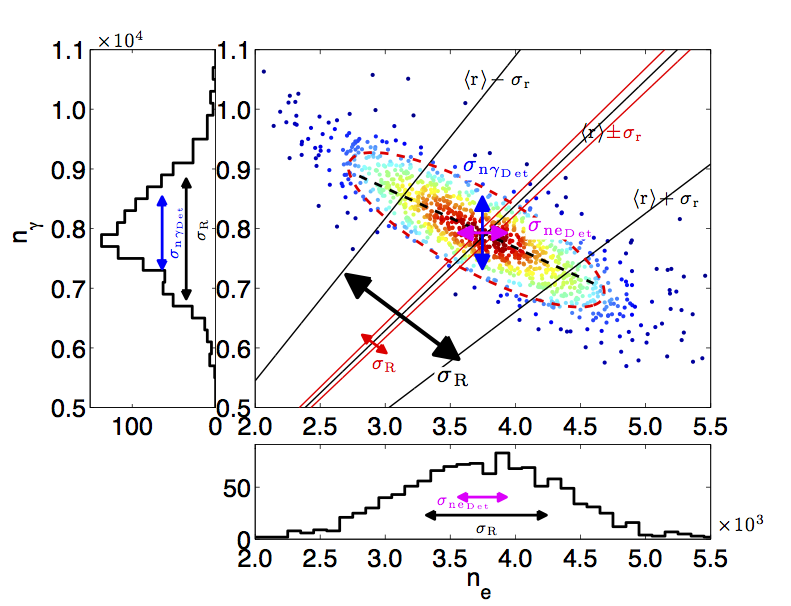
\includegraphics[width=150mm]{Chapter_Flucs/Figures/Ex_Plots/r_fig.png}
\caption{Fluctuations of the 164 keV line from $\rm ^{131}Xe$ in the LUX detector, with the number of electrons plotted vs. the number of photons. The blue and magenta arrows labeled as $\rm \sigma_{n_{\gamma_{Det}}}$ and $\rm \sigma_{n_{e_{Det}}}$ are the size of fluctuations in the light and charge channels due to the resolution of the LUX detector. The black arrow represents the size of recombination fluctuations $\rm \sigma_R$. The value of $\rm \left<r\right>$ is the average observed recombination fraction or the average recombination probability $\rm r_p$. The red lines represent constant $\rm \left<r\right> \pm \sigma_r $ assuming the expected binomial variance of equation \ref{eq:Fano_Intro}. The black lines represent constant $\rm \left<r\right> \pm \sigma_r $ measured from the data. The black dashed line is represent constant energy or constant number of quanta.  }
\label{fig:Flucs_Ex}
\end{figure}
\renewcommand{\baselinestretch}{2}
\small\normalsize

\noindent the blue and magenta arrows labeled as $\rm \sigma_{n_{\gamma_{Det}}}$ and $\rm \sigma_{n_{e_{Det}}}$ are the size of fluctuations in the light and charge measurement due to the resolution of the LUX detector. The value of $\rm \left<r\right>$ is the average observed recombination fraction and can be thought of as the average recombination probability $\rm r_p$. The red lines represent constant $\rm \left<r\right> \pm \sigma_r $ assuming the expected binomial variance of equation \ref{eq:Fano_Intro}. The expected recombination (in red) is small compared to fluctuations from detector resolutions and is more than a factor of ten less than that observed. The black lines represent constant $\rm \left<r\right> \pm \sigma_r $ measured from the data. The size of recombination fluctuations $\rm \sigma_R$ are dominant over detector resolution stretching the island size along lines of constant energy (black dashed line). The island is not stretched exactly along the black dashed line as the non negligible component from detector resolution also warp the population. The projection of the population onto the combined quanta axis $\rm (n_\gamma + n_e)$, or energy E/W, is shown in figure\ref{fig:Flucs_Ex_E}.

\renewcommand{\baselinestretch}{1}
\small\normalsize
\begin{figure}[h!]\centering
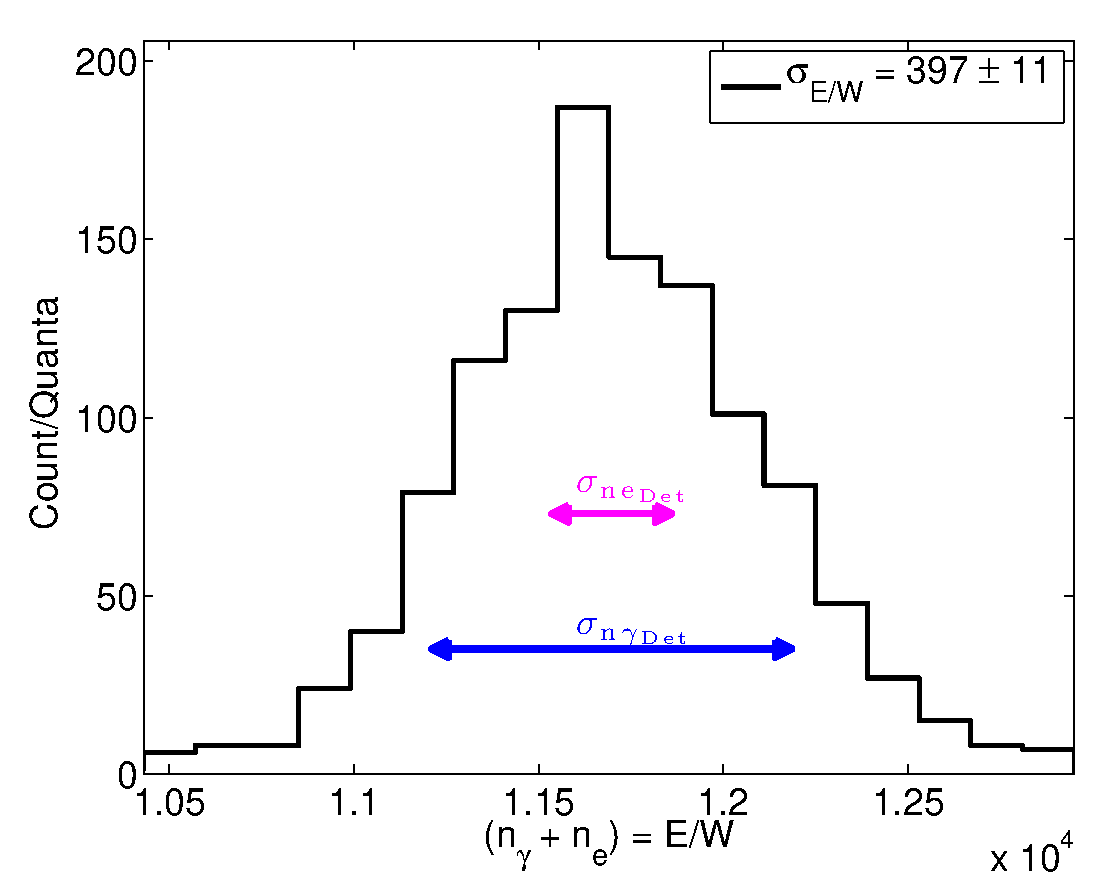
\includegraphics[width=120mm]{Chapter_Flucs/Figures/Ex_Plots/E_fig.eps}
\caption{The projection of the population in figure \ref{fig:Flucs_Ex} onto the combined quanta axis $\rm (n_\gamma + n_e) = E/W$. Along this projection the dominant recombination fluctuations cancel out, leaving on the components from detector resolution $\rm \sigma_{n_{\gamma_{Det}}}$ and $\rm \sigma_{n_{e_{Det}}}$. }
\label{fig:Flucs_Ex_E}
\end{figure}
\renewcommand{\baselinestretch}{2}
\small\normalsize

\noindent In the combined light and charge axis we find that the recombination fluctuations have vanished. Leaving only the statistical variance from detector resolution. Some useful definitions of parameters which will be discussed in this section are given in table \ref{table:Fluc_Param}.

\renewcommand{\baselinestretch}{2}
\small\normalsize
\begin{table}[h!]
\begin{center}
\begin{tabular}{|c|c|c|}
\hline
Parameter & Description & Definition \\ \hline
$\rm n_\gamma$ & Number of photons & $\rm \left<S1\right>/g_1$ \\ \hline
$\rm n_e$ & Number of electrons & $\rm \left<S2\right>/g_2$ \\ \hline
$\rm n_i$ & Number of ions & $\rm (n_\gamma+n_e)/(1+\alpha)$ \\ \hline
$\rm n_{ex}$ & Number of excitons & $\rm \alpha n_{i}$ \\ \hline
$\rm \alpha$ & Exciton to ion ratio & $\rm n_{ex}/n_{i}$ \\ \hline
$\rm \sigma_{n_{\gamma_{Det}}}$ &$\rm n_\gamma$ detector fluctuations & equation \ref{eq:SigDet} \\ \hline
$\rm \sigma_{n_{e_{Det}}}$ &$\rm n_e$ detector fluctuations  & equation \ref{eq:SigDet} \\ \hline
$\rm r$ & Recombination fraction &  $\rm \left(\frac{n_\gamma}{n_e} - \alpha \right)/\left(\frac{n_\gamma}{n_e}+1\right)$ \\ \hline
$\rm r_p$ & Recombination probability & $\rm \left<r\right>$ \\ \hline
R & Recombined ions &  $\rm \left<r\right>n_{i}$ \\ \hline
$\rm \sigma_{R}$ & Recombination fluctuations &  $\rm \sigma_{\left<r\right>}n_{i}$ \\ \hline
\end{tabular}
\caption{LUX detector parameters, used to measure statistical fluctuations in the light (S1) and charge (S2) channels. Where the S1 and S2 signals have been corrected for position dependance outlined in section \ref{Ch:3}. The values of $\rm g_1$ and $\rm g_2$ where measured in section \ref{Ch:E_Scale_Cal}. }
\label{table:Fluc_Param}
\end{center}
\end{table}
\renewcommand{\baselinestretch}{2}
\small\normalsize

For the rest of this section we will build on the example from figure \ref{fig:Flucs_Ex} to better understand recombination fluctuations. We will explore recombination fluctuations with line-source calibrations then expand the picture to deal with continuous sources. 

\newpage

\section{Modeling Intrinsic Detector Resolution}

Intrinsic statistical fluctuations in light and charge (S1 and S2) collection in the LUX detector lead to a spread in collected quanta. To measure effects from recombination fluctuations and the Fano factor, we must first decouple the detector component of resolution. We use the model described in \cite{Platzman} \cite{Dahl_Thesis} in which the measured scintillation and ionization signals (S1 and S2 measured in PE) are related to the number of photons and electrons by gains $\rm g_1$ and $\rm g_2$, equation \ref{eq:Gain1} and \ref{eq:Gain2}. Specifically, the average number of photons and electrons produced for a given energy deposit are proportional to the average S1 and S2 signals.

\begin{alignat}{2}
\label{eq:Gain1} \rm  \left<n_\gamma\right> = \frac{\left<S1\right>}{g_1}\\
\label{eq:Gain2} \rm \left<n_{e}\right> = \frac{\left<S2\right>}{g_2}
\end{alignat}

\noindent where the gain $\rm g_1$ represents photon detection efficiency, the probability of a photon from an energy deposit striking a PMT and producing a photo electron signal (PE). Gain $\rm g_2$ represents the average S2 signal of a single electron multiplied by the electron extraction efficiency $\rm \epsilon$. Here, we are only using the S2 of the bottom PMT array and is corrected for electron-lifetime. The fluctuations in photons and electrons are related to the observables S1 and S2 by equations \ref{eq:Gain1} and \ref{eq:Gain2}

\begin{alignat}{2}
\label{eq:Sig_g1$} \rm  \sigma_{n_{\gamma_{stat}}}^2 = \frac{\sigma_{S1_{stat}}^2}{g_1^2}\\
\label{eq:Sig_g2$} \rm \sigma_{n_{e_{stat}}}^2 = \frac{\sigma_{S2_{stat}}^2}{g_2^2}
\end{alignat}

\noindent where $\rm  \sigma_{n_{\gamma_{stat}}}^2$ and $\rm \sigma_{n_{e_{stat}}}^2$ represent the variance in the average number of measured photons and electrons as measured through S1 and S2, respectively. The variances in S1 and S2, $\rm \sigma_{S1_{stat}}^2$ and $\rm \sigma_{S2_{stat}}^2$, are the observable quantities with the detector. The variance in terms of quanta ($\rm n_\gamma$ and $\rm n_e$) must be considered in terms of the PE being counted by the PMTs. Note, here we are working with the x,y,z corrected signals outlined in section \ref{Ch:3}. 


Before proceeding to derive the statistical variance in light and charge, we overview a list of terms and their values in the LUX detector, given in table \ref{table:LUX_Det_Param}.

\begin{table}[h!]
\begin{center}
\begin{tabular}{|c|c|c|}
\hline
Parameter & Definition & Value
 \\ \hline
$\rm g_1$	& photon detection probability	& 0.097 $\pm$ 0.008 $\rm[PE/n_\gamma]$ \\ \hline
$\rm \sigma_{PE} $ & single PE resolution, all PMTs	& 0.50 $\rm[PE/n_\gamma]$	\\ \hline
$\rm g_2$ = $\rm \epsilon SE_b$	& average electron signal	& 5.75 $\pm$ 1.4 $\rm[PE/n_e]$ \\ \hline
$\rm SE_b$ & single electron size, bottom PMT array & 9.70 $\pm$ 0.1 $\rm [PE/n_e]$ \\ \hline
$\rm \epsilon$ & electron extraction probability & 0.593 $\pm$ 0.144 \\ \hline
$\rm \sigma_{SE_b}$ & single electron resolution, bottom PMT array & 3.6 $\rm [PE/n_e]$ \\ \hline
$\rm \kappa$	& fraction of non-attenuated electrons & 0.85 \\ \hline
\end{tabular}
\caption{LUX detector parameters, used to measure statistical fluctuations in the light (S1) and charge (S2) channels. Where the S1 and S2 signals have been corrected for position dependance outlined in section \ref{Ch:3}. The values of $\rm g_1$ and $\rm g_2$ where measured in section \ref{Ch:E_Scale_Cal}. }
\label{table:LUX_Det_Param}
\end{center}
\end{table}


The statistical variance of the x,y,z corrected S1 signal, in equation \ref{eq:Sig_1}, can be broken into two linearly independent parts. First we consider the binomial variance, for each event there are $\rm n_\gamma$ number of PE to be collected by the PMTs with probability $\rm g_1$. Here, $\rm n_\gamma$ should be thought of as the number of trials. The binomial variance is,
\begin{equation}
\rm \sigma_{S1_{Bino}}^2 = (1-g_1) g_1 n_\gamma
\label{eq:S1_bino} 
\end{equation}
\noindent where $\rm \sigma_{S1_{Bino}}^2$ is the binomial variance of the S1 light collection process with probability $\rm g_1$ and $\rm n_\gamma$ number of trials. Each PE that was collected by a PMT then undergoes a second fluctuation due to the resolution of the PMTs. The variance from PMT resolution can be written as
\begin{equation}
\rm \sigma_{S1_{PMT}}^2 = g_1 n_\gamma \sigma_{PE}^2
\label{eq:S1_pmt}
\end{equation}
\noindent where $\rm \sigma_{S1_{PMT}}^2$ is the average variance due to PMT resolution. The average single PE resolution of the PMTs is $\rm \sigma_{PE}^2$ and is multiplied by the number of PE collected, $\rm g_1n_\gamma$. 


Combining the two linearly independent processes of equation \ref{eq:S1_bino} and \ref{eq:S1_pmt} leads to the the result in equation \ref{eq:Sig_S1}.
\begin{equation}
\rm  \sigma_{S1_{stat}}^2 = (1-g_1+\sigma_{PE}^2) (g_1 n_\gamma) = (1-g_1+\sigma_{PE}^2) S1 \\ 
\label{eq:Sig_S1}
\end{equation}

\noindent where $\rm \sigma_{S1_{stat}}^2 $ is the statistical variance of the S1 signal. The variance in the measured number of photons is then equation \ref{eq:Sig_S1} divided by $\rm g_1^2$, using equation \ref{eq:Sig_g1$}.
\begin{equation}
\rm  \sigma_{n_{\gamma_{stat}}}^2 = \frac{(1-g_1+\sigma_{PE}^2)}{g_1} n_\gamma \\ 
\label{eq:Sig_Ng}
\end{equation}

We test equation \ref{eq:Sig_S1} and \ref{eq:Sig_Ng} by using the 9.4 $\rm keV$ S1 signal from \KrCal. At that energy the dominant fluctuation is due the statistical variance of light collection, we can ignore contributions from recombination fluctuations and instrumental fluctuations (will be discussed later in this section). The S1 signal is shown in figure \ref{fig:S1_9_Kr}.

\begin{figure}[h!]\centering
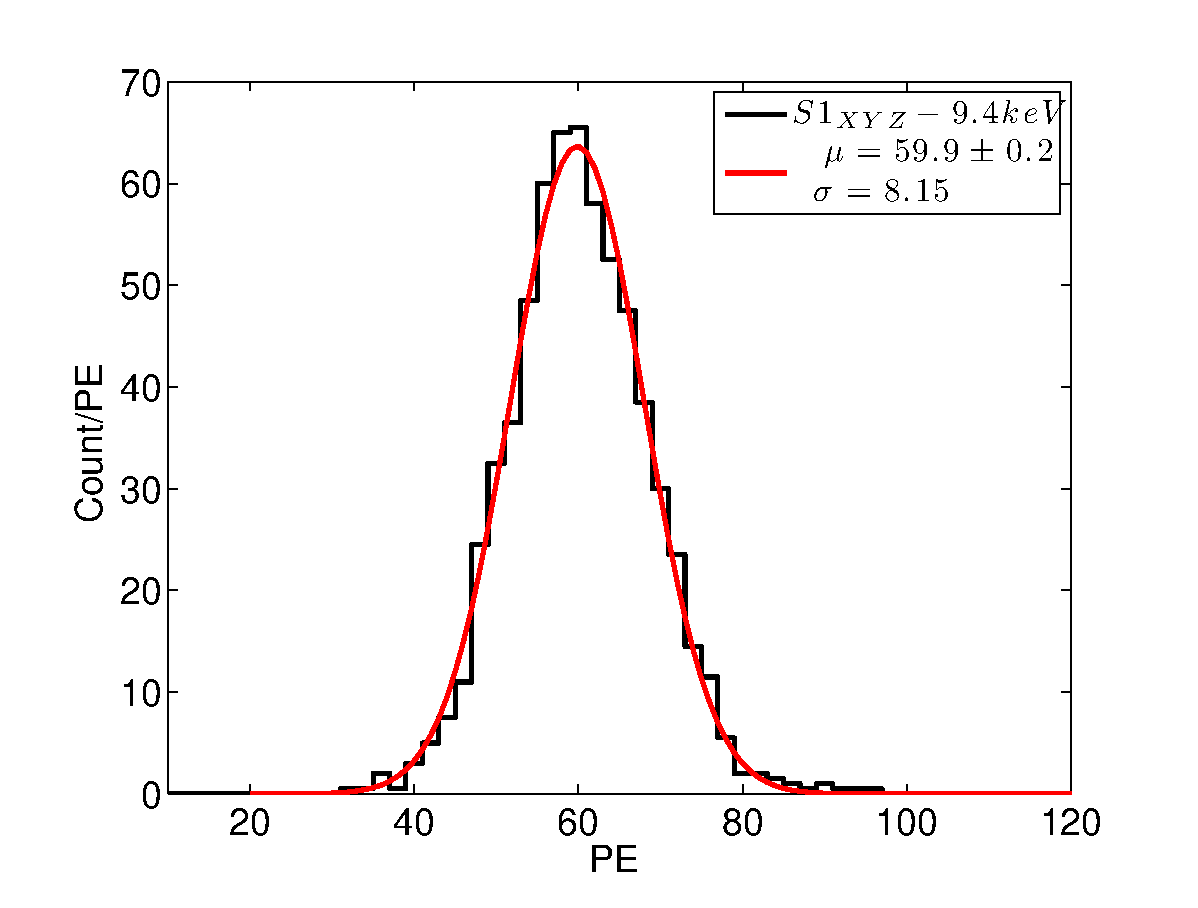
\includegraphics[width=100mm]{Chapter_Flucs//Figures/S1_9_Fluc/S1_9_corr_1000_lux10_20130510T1250_cp09323.eps}
\caption{The fluctuations in the S1-x,y,z corrected signal for the 9.4 keV from \KrCal. At 9.4 keV the statistical variance is dominate over recombination fluctuations, $\rm \sigma_{S1}=8.15$. The resolution is consistent with that expected from statistical fluctuations of 8.3 $\pm$ 0.1 PE, from equation \ref{eq:Sig_S1}. }
\label{fig:S1_9_Kr}
\end{figure}

\newpage

\noindent We find that the observed $\rm \sigma_{S1}$ = 8.15 PE is in good agreement with the expectation from equation \ref{eq:Sig_S1} of 8.3 $\pm$ 0.1 PE. Or in terms of photons, $\rm \sigma_{n_{\gamma_{stat}}}$ = 84.1 with the expectation from equation \ref{eq:Sig_Ng} of 85.7 $\pm$ 1. Having used the values listed in table \ref{table:LUX_Det_Param}.


The variance of the x,y,z corrected S2 signal, given in \ref{eq:Sig_g2$},  is also comprised of several independent processes. Each electron that reaches the liquid-gas interface without being attenuated will either be extracted into the gas producing $\rm SE_b$ number of PE or not. The binomial variance of such a process is,

\begin{equation}
\rm \sigma_{S2_{bino}}^2= (1-\epsilon) \epsilon (\kappa n_e) SE_{b}^2 
\label{eq:Sig_S2}
\end{equation}

\noindent where $\rm \epsilon$ is the electron extraction probability, and $\rm \kappa n_e$ is the average number of electrons that reach the liquid surface from the interaction site, also the number of trials. Recalling that $\kappa$ is the average electron probability of an electron to not be attenuated. For the case of LUX with an electron lifetime of $\sim 1000 \, \mu s$ and an average drift time of 160 $\rm  \mu s$ the value of $\rm \kappa$ = 0.85 and is listed in table \ref{table:LUX_Det_Param}. Each electron that gets extracted then multiplies producing $\rm SE_b$ PE in the bottom PMT array, this multiplicative factor must be squared in the variance. 

Next, we consider the spread of the single electron size as measured by the bottom PMT array, $\rm \sigma_{SE_{b}}$. The variance from the PMT resolution for the $\rm \epsilon (\kappa n_e)$ number of electrons extracted is,
\begin{equation}
\rm \sigma_{S2_{PMT}}^2 = \epsilon (\kappa n_e)  \sigma_{SE}^2
\label{eq:S2_PMT}
\end{equation}

\noindent where $\rm \epsilon \kappa n_e$ is the number of extracted electrons each with PMT resolution $\rm \sigma_{SE}^2$.

For the S2 signal we must also consider the additional variance from electron attenuation as the electrons drift, we model the process with a Poisson probability of electron capture in each Z slice of the detector. The variance from each Z slice depends of the average number of electrons that will be attenuated. The probability of attenuation at each slice in drift-time T is $\rm P(T)= 1-e^{-T/\tau}$, where $\rm \tau$ for the data sets to be considered is 1000 $\rm \mu s$. The drift region considered in the fiducial volume is from 38 to 304.5 $\rm \mu s$. The average variance from events in the fiducial can be given by equation \ref{eq:Sig_Att}.

\begin{equation}
\rm  \sigma_{n_{e_{att}}}^2 = n_e \frac{\mathlarger{\int}\limits_{\mathsmaller{T_{min}}}^{\mathsmaller{T_{max}}} (1-e^{-T/\tau})\mathrm{d}T}{\mathlarger{\int}\limits_{\mathsmaller{T_{min}}}^{\mathsmaller{T_{max}}}\mathrm{d}T} = 0.155 \times n_e
\label{eq:Sig_Att}
\end{equation}

Combining the variances from equations \ref{eq:Sig_S2} \ref{eq:S2_PMT} and \ref{eq:Sig_Att} leads to the the result for the statistical variance in the observed S2 signal,

\begin{equation}
\begin{split}
\rm  \sigma_{S2_{stat}}^2 = (1-\epsilon)\epsilon  (\kappa n_e) SE_b^2 + \epsilon  (\kappa n_e) \sigma_{SE}^2+  g_2^2 \sigma_{n_{e_{att}}}^2 \\
\rm  \sigma_{S2_{stat}}^2= \left((1-\epsilon) SE_b \kappa + \sigma_{SE}^2 \kappa/g_2+  0.155 g_2\right)S2\\
\label{eq:Sig_S2}
\end{split}
\end{equation}

\begin{equation}
\rm  \sigma_{n_{e_{stat}}}^2 = \frac{(1-\epsilon)\epsilon SE_b^2 + \epsilon  \sigma_{SE}^2}{g_2^2} \kappa n_e+  \sigma_{n_{e_{att}}}^2 \\
\label{eq:Sig_Ne}
\end{equation}


%For this analysis we use the following detector gains: \ref{eq:$\rm g_1$$\rm g_2$}. 
%\begin{multline} \\
%\rm g_1 = 0.097 \pm 0.008 \,[PE/n_\gamma]\\
%\rm g_2=SE_{b} \times \epsilon = 5.75 \pm 1.4 \,[PE/n_e]\\
%\rm SE_{b} = 9.70 \pm 0.05  \,[PE/n_e] \\\ 
%\rm \sigma_{SE_b} = 3.64\, [PE/n_e]\\
%\rm \Gamma = \left<n_{e_z0}\right>/\left<n_e\right>=0.85 \\
%\rm \epsilon = 0.593\pm 0.144 \\
%\rm \sigma_{PE} = 0.51\, [PE/n_\gamma]\\\
%\label{eq:$\rm g_1$$\rm g_2$}
%\end{multline}

Using equations \ref{eq:Sig_Ng}, \ref{eq:Sig_Ne} and table \ref{table:LUX_Det_Param} we calculate the intrinsic detector resolution for S1 and S2 signals in the LUX detector, given equation \ref{eq:SigStat}. Note, the intrinsic resolution in S2 is subdominant to that of S1, since  on average one electron multiplies to about ten photons detected by the bottom PMT array. Also listed in \ref{eq:SigInst}, are the instrumental fluctuations with a linear dependance on quanta measured using calibrations discussed in section \ref{sec:flucs_mono}. The total variance that the detector observes in the light and charge is the linear combination of the statistical and instrumental variance given in equation {eq:SigDet}.  

\begin{equation}
\begin{split}
\rm  \sigma_{n_{\gamma_{stat}}} = 3.45\pm_{0.15}^{0.17} \sqrt{n_\gamma}\\
\rm \sigma_{n_{e_{stat}}} = 0.68\pm_{0.20}^{0.26} \sqrt{n_e}
\label{eq:SigStat}
\end{split}
\end{equation}

\noindent where  $\rm \sigma_{n_{\gamma_{stat}}}$ and $\rm \sigma_{n_{e_{stat}}}$ are the statistical fluctuations outlined in this section.

\begin{equation}
\begin{split}
\rm  \sigma_{n_{\gamma_{inst}}} = \frac{6.4\pm 1.7}{100} \times n_\gamma\\
\rm  \sigma_{n_{e_{inst}}} = \frac{6.6\pm 0.9}{100} \times n_e
\label{eq:SigInst}
\end{split}
\end{equation}

\noindent where  $\rm \sigma_{n_{\gamma_{inst}}}$ and $\rm \sigma_{n_{e_{inst}}}$ are instrumental fluctuations extracted in section \ref{sec:flucs_mono} that grow like number of quanta n but only appear to turn on above 200 keV.

\begin{equation}
\begin{split}
\rm  \sigma_{n_{\gamma_{Det}}}^2 = \sigma_{n_{\gamma_{stat}}}^2 + \sigma_{n_{\gamma_{inst}}}^2 \\
\rm \sigma_{n_{e_{Det}}}^2 = \sigma_{n_{e_{stat}}}^2 + \sigma_{n_{e_{inst}}}^2
\label{eq:SigDet}
\end{split}
\end{equation}

\noindent where  $\rm \sigma_{n_{\gamma_{Det}}}^2$ and $\rm \sigma_{n_{e_{Det}}}^2$ are the fluctuations in counting photons and electrons, respectively, due to detector resolution.


\section{Measuring Recombination Fluctuations with Mono-Energetic Sources}
\label{sec:flucs_mono}

To model recombination we start with the assumption that for a given energy deposit in liquid xenon the number of quanta produced is equal to the number of excitons and the number of ions \cite{Platzman}. 

\begin{equation}
\begin{split}
\rm  \frac{E}{W} = n_q = n_i + n_{ex} = n_i(1+\alpha) \\
\rm \frac{E}{W} = n_\gamma + n_e = \frac{n_\gamma}{g_1} + \frac{n_e}{g_2} \\
\label{eq:Energy}
\end{split}
\end{equation}

\noindent where E is energy in keV, W is the work function in keV/quanta, $\rm n_{q}$ is the number of quanta, $\rm n_{i}$ is the number of ions, $\rm n_{ex}$ is the number of excitons and and $\rm \alpha$ is the exciton-to-ion ratio. The theoretical value of the number of excitons produced to ions is $\rm \frac{n_{ex}}{n_{i}}= \alpha = 0.20$ \cite{Doke_alpha} and is not expected to change as a function of energy \cite{alpha_argon} \cite{alpha_xenon} \cite{Dahl_Thesis}. For the subsequent equations in this section we will simplify equations \ref{eq:Energy} to,

\begin{equation}
\begin{split}
\rm \alpha = 0.20\\
\rm  n_i = \frac{E}{W} \frac{1}{(1+\alpha)} =  \frac{n_\gamma + n_e}{(1+\alpha)}  \\ %  \frac{n_q}{(1+\alpha)}
\label{eq:Energy_2}
\end{split}
\end{equation}

\noindent Equation \ref{eq:Energy_2} gives us a simple model for the number of ions produced for a given interaction. We work in number of ions for convince as the recombination fluctuations act only on ions. The only variation in quanta thus far is due to a Fano factor governing the variation in initial quanta produced. 
\begin{equation}
\rm \sigma_{n_i}^2  = F \times n_i
\label{eq:Fano_1}
\end{equation}

\noindent where F is the Fano factor. The value of F for liquid xenon is small and has a theoretical value of 0.05 \cite{FanoTheoretical}.


We now describe the observed scintillation and ionization signals that are measured in the LUX detector, S1  and S2 respectively, as a function of $\rm n_i$. The number of photons observed for a given energy deposit arise from the excitons that de-excite and from ions which recombine with freed electrons.
\begin{equation}
\rm  n_\gamma = n_{ex} + n_i\times r = n_i\times (r+\alpha) \\
\label{eq:Photons}
\end{equation}

\noindent The number of electrons corresponding to a given energy deposit is equal to the number of ions that did not recombine with a freed electron. 

\begin{equation}
\rm  n_e = n_i\times (1-r)\\
\label{eq:Electrons}
\end{equation}

\noindent The recombination fraction of each event can be solved for interns of number of photons and electrons produced,

\begin{equation}
\rm r= \frac{\frac{n_\gamma}{n_e}-\alpha}{\frac{n_\gamma}{n_e} + 1}
\label{eq:recomb_frac}
\end{equation}

\noindent where r represents the electron-ion recombination probability of each event. 

Two key measurable quantities from the scintillation and ionization signals are the average recombination fraction $\rm \left<r\right>$ and the spread in recombination probability $\rm \sigma_{\left<r\right>}$. The average recombination fraction $\rm \left<r\right>$ can be interpreted as the electron-ion pair recombination probability $\rm r_p$. The recombination fluctuation in units of quanta is 
\begin{equation}
\rm \sigma_R = \rm \sigma_{\left<r\right>} \times n_i
\label{eq:R_eq}
\end{equation}
\noindent where $\rm \sigma_R$ is the recombination fluctuation. As mentioned earlier, the recombination fluctuations are much larger than those expected from the binomial variance of a binomial process with probability $\rm r_p$ or the Fano factor, illustrated in figure \ref{fig:Flucs_Ex}.


 We now combine the variance from the Fano factor, recombination and detector resolution (equation \ref{eq:SigDet}) and solve for the total observed variance in photons and electrons given in \ref{eq:SigR_g} and \ref{eq:SigR_e}

\begin{alignat}{2}
\label{eq:SigR_g} \rm \sigma_{n_\gamma}^2  =\sigma_{n_{ex}}^2 + \sigma_{n_i}^2 r_p^2 +  \sigma_{\left<r\right>}^2 n_i^2 +\sigma_{n_{\gamma_{Det}}}^2 =  [\sigma_{n_{ex}}^2 + n_iF r_p^2] + \sigma_{\left<r\right>}^2 n_i^2 + \sigma_{n_{\gamma_{Det}}}^2 \\
\label{eq:SigR_e} \rm \sigma_{n_e}^2  = \sigma_{n_i}^2 (1-r_p)^2 +  \sigma_{\left<r\right>}^2 n_i^2 +\sigma_{n_{e_{Det}}}^2= [n_iF(1-r)^2]+ \sigma_{\left<r\right>}^2 n_i^2 +\sigma_{n_{e_{Det}}}^2
\end{alignat}

\noindent where $\rm \sigma_{n_{ex}}^2$ is the variance in exciton production, F is the Fano factor, the term $\rm \sigma_{\left<r\right>}^2 n_i^2$ is the recombination fluctuation $\rm \sigma_R$ and the rest of the variables are described in table \ref{table:Fluc_Param}. 

Using a line source, we measure combined energy (equation \ref{eq:Energy}) and $\rm \sigma_{n_\gamma}^2$, $\rm \sigma_{n_e}^2$ and $\rm \sigma_{E}^2$. Dropping the contribution form the Fano factor and the the number of excitons in equations \ref{eq:SigR_g} and \ref{eq:SigR_e} the variance of $\rm \sigma_{n_\gamma}^2$ and $\rm \sigma_{n_e}^2$ is a linear combination of detector resolution and recombination fluctuations.

\begin{alignat}{2}
\label{eq:SigQ_g} \rm  \sigma_{n_{\gamma}}^2 = \sigma_{n_{\gamma_{Det}}}^2 + \sigma{R^2}\\
\label{eq:SigQ_e} \rm \sigma_{n_{e}}^2 = \sigma_{n_{e_{Det}}}^2 + \sigma{R^2}
\end{alignat}

\noindent this concept is illustrated in figure \ref{fig:Flucs_Ex}. The value of recombination fluctuation $\rm \sigma_R$ can be determined by rearranging equations \ref{eq:SigQ_g} and \ref{eq:SigQ_e}. As shown in figure \ref{fig:Flucs_Ex_E}, when the light and charge signals are combined the rustling variance $\rm \sigma_{E}^2$ contains no recombination fluctuations, as recombination fluctuations are 100\% anti-correlated in light and charge. 
\begin{equation}
\rm \sigma_{R}^2  = \frac{1}{2}\left(\sigma_{n_\gamma}^2 + \sigma_{n_e}^2 - \frac{\sigma_E^2}{W^2}\right)\\
\label{eq:Dahl}
\end{equation}

\noindent where the variance in photons $\rm \sigma_{n_\gamma}^2$, electrons $\rm  \sigma_{n_e}^2$  and quanta $\rm \frac{\sigma_E^2}{W^2}$ are all observable quantities with a line source. And can be rewrite in terms of the observable quantities S1 and S2.

\begin{equation}
\rm \sigma_{R}^2  = \frac{1}{2}\left( \frac{\sigma_{S1}^2}{g_1^2} + \frac{\sigma_{S2}^2}{g_2^2} - \frac{\sigma_E^2}{W^2}\right)\\
\label{eq:Dahl_2}
\end{equation}

\noindent We now have a method to extract the recombination fluctuation $\rm \sigma_R$ using a line calibration source. To complete our treatment of line sources, the variance in the light and charge due to detector resolution can also be measured.

\begin{alignat}{2}
\label{eq:SigQ_S1} \rm  \sigma_{n_{\gamma_{Det}}}^2 = \frac{\sigma_{S1}^2}{g_1^2} - \sigma{R^2}\\
\label{eq:SigQ_S2} \rm \sigma_{n_{e_{Det}}}^2 = \frac{\sigma_{S2}^2}{g_2^2} - \sigma{R^2}
\end{alignat}


Using equation \ref{eq:Dahl_2}, \ref{eq:SigQ_S1} and \ref{eq:SigQ_S2} along with the measurements of $\rm g_1$ $\rm g_2$, we construct a combined energy and deconvolve the recombination fluctuations from variances in the light and charge observed by the detector. The result is shown in figure \ref{fig:E_dis}, The black white and red lines represent $\rm \sigma_R, \, \sigma_{n_{\gamma_{Det}}}, \,\sigma_{n_{e_{Det}}}$, respectively. With the values and sources listed in table \ref{table:Line_Data}.

\renewcommand{\baselinestretch}{1}
\small\normalsize
 \begin{figure}[h!]\centering
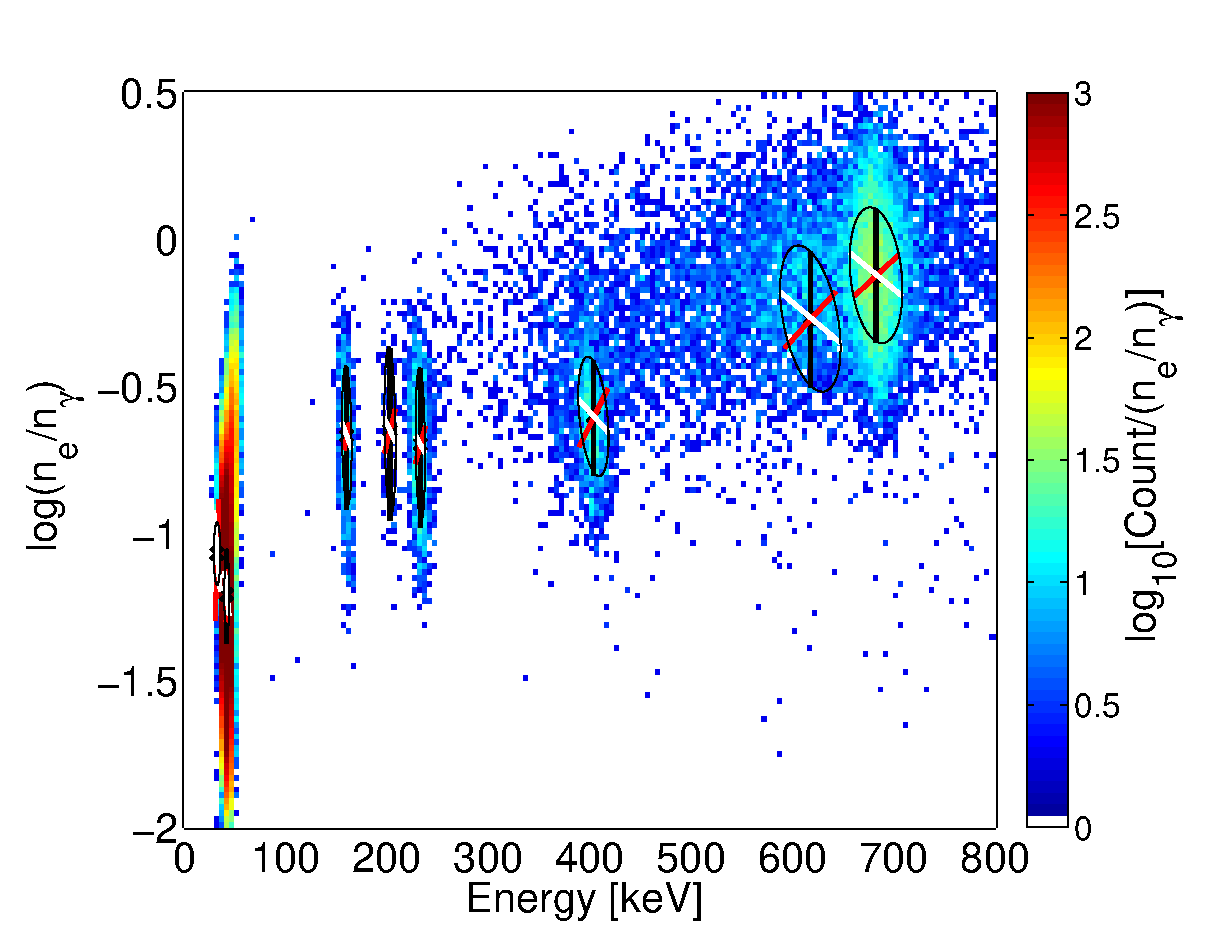
\includegraphics[width=130mm]{Chapter_Flucs/Figures/All_disc.eps}
\caption{Populations of calibration sources in discrimination space $\rm log\left(\frac{n_e}{n_\gamma}\right) $ vs. combined energy $\rm keV_{ee}$. The ovals represent the combination of $\rm \sigma_R, \, \sigma_{n_{\gamma_{Det}}}, \,\sigma_{n_{e_{Det}}} $ in black, white, red respectively.}
\label{fig:E_dis}
\end{figure}
\renewcommand{\baselinestretch}{2}
\small\normalsize

\renewcommand{\baselinestretch}{1}
\small\normalsize
\begin{table}[h!]
\begin{center}
\begin{tabular}{|c|c|c|c|c|c|} \hline
Source & Energy & $\rm \sigma_R$ &  $\rm \sigma_{n_{\gamma_{Det}}}$ &  $\rm \sigma_{n_{e_{Det}}}$ & $\rm \sigma_E/W$  \\
& [keV] & & & & \\ [0.5ex] % inserts table %heading
\hline
K-shell X-ray 				& $\sim$32 	 &  52.6 $\pm$ 23 		& 244 $\pm$ 5		& 116 $\pm$ 3 		 & 269 $\pm$ 5						\\ \hline
 $\rm ^{83m}Kr$ 				& 41.55		& 82.4	$\pm$ 0.6			& 171 $\pm$ 0.3		& 51.2 $\pm$	0.3		& 173 $\pm$ 0.2				\\ \hline
 $\rm ^{131}Xe$ 				& 163.9		& 637 $\pm$ 20			& 388	$\pm$ 31		& 83 $\pm$ 77		& 375 $\pm$ 8				\\ \hline
$\rm ^{127}Xe$ 				& 208.3 		& 916	$\pm$ 59			& 506	$\pm$ 96 		& 260 $\pm$ 133	 	& 568 $\pm$ 26			\\ \hline
$\rm ^{127}Xe, ^{129m}Xe$	 & 236.8		& 1001 $\pm$ 23			& 441	$\pm$ 50		& 253 $\pm$ 71		& 491 $\pm$ 9				\\ \hline
$\rm ^{127}Xe$			  	 & 408.8		& 1294 $\pm$ 44			& 1166	 $\pm$ 39		& 949 $\pm$ 40		& 1562 $\pm$ 22			\\ \hline
$\rm ^{214}Bi	$				& 609 			& 2488 $\pm$ 109		& 2298 $\pm$ 99		& 1627 $\pm$ 107	& 3291 $\pm$ 60				 \\ \hline
$\rm ^{137}Cs$				& 661.6		& 2686 $\pm$ 34			& 2059 $\pm$ 38		& 1368 $\pm$ 46		& 2564 $\pm$ 17				\\ [0.5ex] 
\hline
\end{tabular}
\caption{ Extracted fluctuations from the line source calibration data in units of quanta. The method of extracting the quantities is given in \ref{eq:Dahl_2}, \ref{eq:SigQ_S1} and \ref{eq:SigQ_S2} and illustrated for the case of  $\rm ^{131}Xe$ in figures \ref{fig:Flucs_Ex} and \ref{fig:Flucs_Ex_E}. Note, the K-shell X-ray may include a fairly large systematic as no radial cut was made in order to observe the signal near the detector edge.}
\label{table:Line_Data}
\end{center}
\end{table}
\renewcommand{\baselinestretch}{2}
\small\normalsize

\noindent The values of $\rm \sigma_R, \, \sigma n_{\gamma_{Det}}, \,\sigma n_{e_{Det}} $ from table \ref{table:Line_Data} are plotted in figure \ref{fig:Flucs}.

\renewcommand{\baselinestretch}{1}
\small\normalsize
 \begin{figure}[h!]\centering
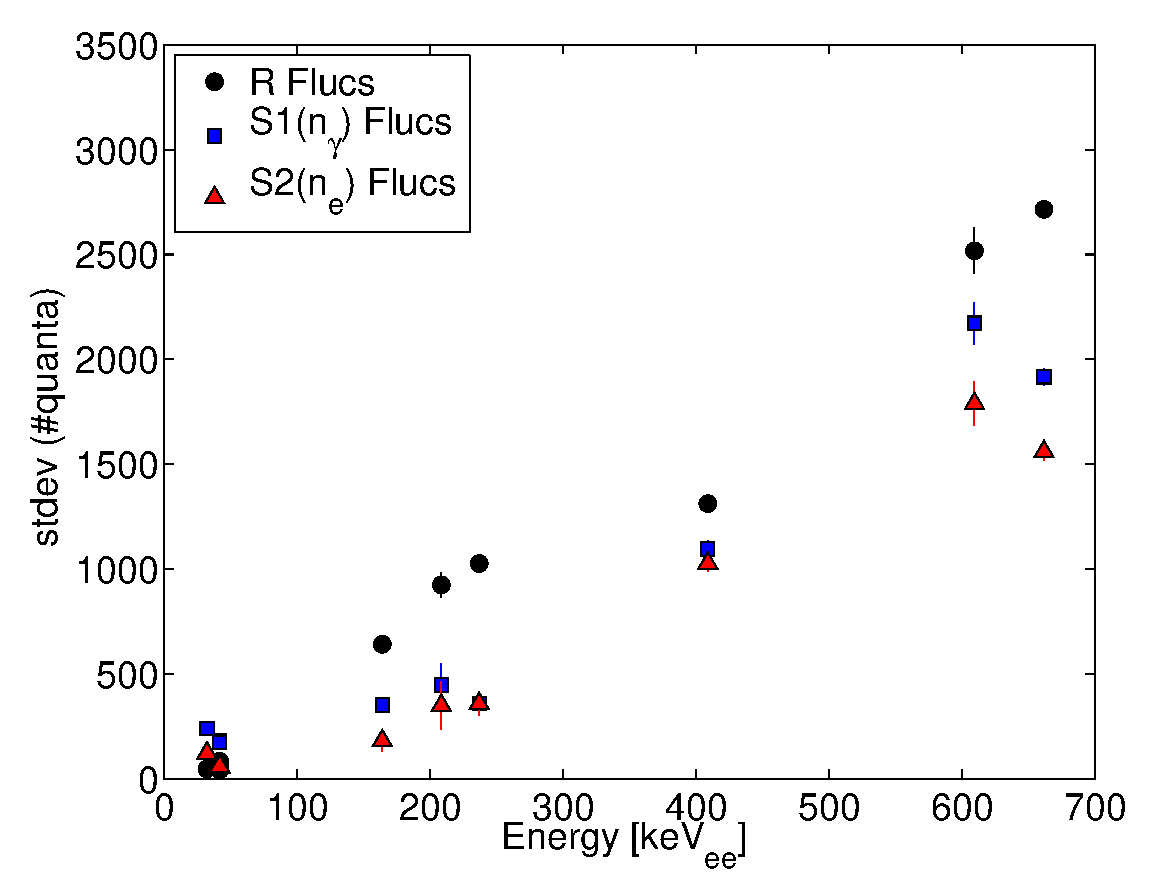
\includegraphics[width=70mm]{Chapter_Flucs/Figures/fluc_E.eps}
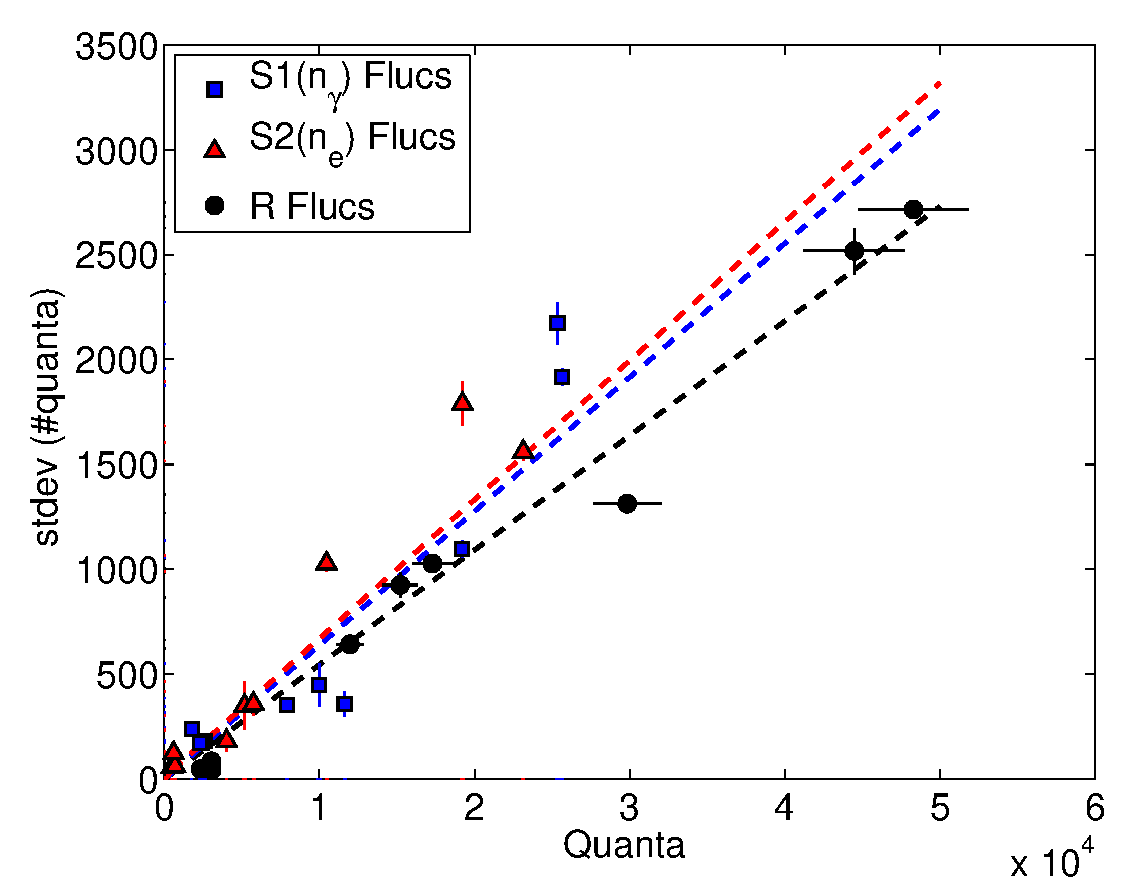
\includegraphics[width=70mm]{Chapter_Flucs/Figures/fluc_Q.eps}
\caption{Measured values of $\rm \sigma_R, \, \sigma n_{\gamma_{Det}}, \,\sigma n_{e_{Det}} $ vs. Energy on the left and vs. quanta in photons, electrons and ions, respectively,  on the right. Measured using sources listed in Table \ref{table:Line_Data}. }
\label{fig:Flucs}
\end{figure}
\renewcommand{\baselinestretch}{2}
\small\normalsize

A variance with a linear and root term is fit to the data with the results given in \ref{eq:Inst_Fit}. The linear term corresponds to instrumental fluctuations and the root term corresponds to statistical fluctuations. Instrumental fluctuations are proportional to the signal size and cause the fluctuations in $\rm \sigma n_{\gamma_{Det}}, \,\sigma n_{e_{Det}} $ at high energies to deviate from statistical fluctuations alone. 

\begin{equation}
\begin{split}
\rm  \sigma_{n_{\gamma_{Det}}}^2 = \sigma_{n_{\gamma_{Stat}}}^2 + \sigma_{n_{\gamma_{Inst}}}^2 =\left(0 \pm10\cdot \sqrt{n_\gamma}\right)^2 + \left((6.4\pm1.8)/100\cdot n_\gamma\right)^2 \\
\rm \sigma_{n_{e_{Det}}}^2 = \sigma_{n_{e_{Stat}}}^2 + \sigma_{n_{e_{Inst}}}^2 = \left(1\pm4\cdot \sqrt{n_e}\right)^2 + \left((6.6\pm0.6)/100\cdot n_e\right)^2 \\
\rm \sigma_R^2=   \left((5.5\pm0.5)/100\cdot n_q\right)^2
\label{eq:Inst_Fit}
\end{split}
\end{equation}

\noindent With the limited data we can not tightly constrain the root-n term. The statistical fluctuation expected from equation \ref{eq:SigStat} is consistent with the observed values without the instrumental component for calibration energies at and below 236.8 keV. The instrumental fluctuations appear to turn on above $\sim$200 keV and may be due to and may be due to ripples in the liquid surface caused by xenon bubbles or other systematics. 


\section{Measuring Recombination Fluctuations in Disecrate Energy Bins}
\label{sec:flucs_mono_bins}

The pervious section demonstrated the power of using a mono energetic source measure recombination fluctuations, equation  \ref{eq:Dahl_2}. In this section we present a method to decouple statistical variance from recombination fluctuations when confined to an energy bin of width $\rm \Delta_E$. The consideration of desecrate binning is crucial when dealing with a continual energy spectrum. Take the tritium beta spectrum as an example, we lose the ability to independently measure $\rm \sigma_{n_\gamma}^2$, $\rm \sigma_{n_e}^2$, $\rm \sigma_{E}^2 $ and are only left with a smear of $\rm n_\gamma$, $\rm n_e$, $\rm E $. However, there are two key pieces of information still left at our disposal. First, the combined energy can be reconstructed from constraints on $\rm g_1$ and $\rm g_2$, and even corrected for spectral shape and detector resolution (discussed later in section \ref{sec:Smear}). Second, we can have determined the detector resolution for the light and charge channels as a function of quanta, described in \ref{eq:SigStat},  \ref{eq:SigInst}. It will be shown in this section knowing $\rm g_1$, $\rm g_2$ and the intrinsic detector resolution will be sufficient to measure recombination fluctuations for a continual energy spectrum. 
%binned in energy with width $\rm \Delta_E$.

To simplify the picture we introduce new variables when dealing with events which have been cut from and energy bin of width $\rm \Delta_E$.  After making the cut in energy we call the remaining variance projected onto light and charge $\chi_{n_{\gamma}}^2$ and $\chi_{n_{e}}^2$, which is analogous to $\sigma_{n_{\gamma}}^2$ and $\sigma_{n_{e}}^2$ of equations \ref{eq:SigQ_g} \ref{eq:SigQ_e}, respectively. We denote the component of variance from detector resolution contained in the slice of energy as $\rm \chi_{Det}$. These concepts will be clarified in the subsequent examples and are summarized in table 

\renewcommand{\baselinestretch}{1}
\small\normalsize
\begin{table}[h!]
\begin{center}
\begin{tabular}{|c|c|c|}
\hline
Parameter & Definition & Analogy Without Binning
 \\ \hline
$\rm \chi_{n_{\gamma}}^2$	& Total variance with E cut	& $\sigma_{n_{\gamma}}^2$ \\ 
							& projected onto $\rm n_\gamma$ & 						\\ \hline					
$\rm \chi_{n_{e}}^2$ & Total variance with E cut	& $\rm \sigma_{n_{e}}^2$	\\
							& projected onto $\rm n_e$ & 						\\ \hline
$\rm \chi_{Det}^2$			& Variance from detector resolution & $\rm \sigma_{n_{\gamma_{Det}}}^2 \, \sigma_{n_{e_{Det}}}^2 $ \\
							& shared between $\rm n_\gamma$ and $\rm n_e$, with E cut   & 						\\ \hline
\end{tabular}
\caption{ Useful definitions when considering cutting events in a bin of energy and projecting onto the $\rm n_\gamma$ and $\rm n_e$ axis. }
\label{table:E_Slice}
\end{center}
\end{table}
\renewcommand{\baselinestretch}{2}
\small\normalsize
 
 \newpage

We begin the treatment of binning by considering several cases using a simulated \KrCal line-source. For each case, we reconstruct the energy using equation \ref {eq:Energy} and make a cut in energy of width $\rm \Delta_E=1$ about the center. First, we turn off detector resolution only leaving recombination fluctuations of $\rm \sigma_R = 83 $, similar to the value extracted from the \KrCal data in table \ref{table:Line_Data}. Figure \ref{fig:Kr_ex_R} shows the result of such a system, with infinite detector resolution and only recombination fluctuations.

\renewcommand{\baselinestretch}{1}
\small\normalsize
 \begin{figure}[h!]\centering
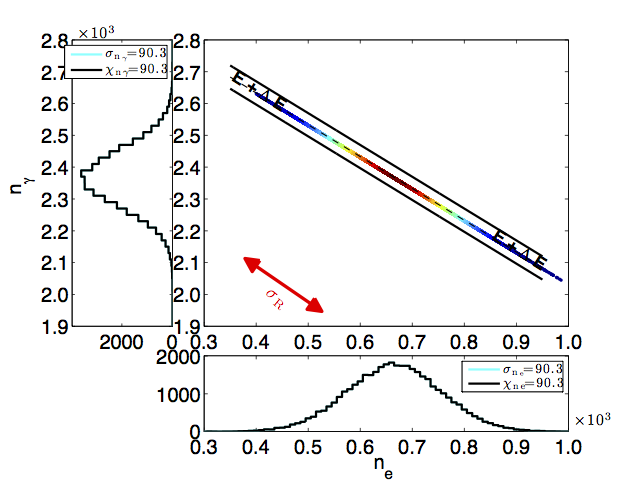
\includegraphics[width=160mm]{Chapter_Flucs/Figures/Ex_Plots/EX_R_Kr_.png}
\caption{A simulated \KrCal source with infinite detector resolution and recombination fluctuations set to 83 quanta. The recombination fluctuation move along the line of constant energy about the center shown in black with a bin width of $\rm \Delta_E$ =1 (back dashed lines). The events are cut between the black dashed lines and projected onto the $\rm n_\gamma$ and $\rm n_e$ axes. The observed variance in light and charge are $\rm \chi_{n_{\gamma}}^2 = \sigma_{n_{\gamma}}^2 = \sigma_{R}^2$ and $\rm \chi_{n_{e}}^2 = \sigma_{n_{e}}^2 = \sigma_{R}^2$.  }
\label{fig:Kr_ex_R}
\end{figure}
\renewcommand{\baselinestretch}{2}
\small\normalsize

\noindent In figure \ref{fig:Kr_ex_R} we see that recombination fluctuations move events along the diagonal of constant energy. The events are cut between the black dashed lines ,representing a bin of energy about the center having width $\rm \Delta_E$ = 1, and are projected onto the $\rm n_\gamma$ and $\rm n_e$ axes. The observed variance in light and charge are $\rm \chi_{n_{\gamma}}^2 = \sigma_{n_{\gamma}}^2 = \sigma_{R}^2$ and $\rm \chi_{n_{e}}^2 = \sigma_{n_{e}}^2 = \sigma_{R}^2$. The key point demonstrated in figure \ref{fig:Kr_ex_R} is that all contribution from recombination fluctuations are included when slicing out a section of energy about the center, no matter how thin we make the slice. Note, the population becomes a delta function in energy about the central value.

Next, we visualize how the intrinsic detector resolution ($\rm \sigma_{n_{\gamma_{Det}}}^2 \,and\, \sigma_{n_{e_{Det}}}^2 $) appears in an energy bin of width $\rm \Delta_E$ for a \KrCal source. The recombination fluctuations are set to zero and the fluctuations from detector resolution are set to $\rm \sigma_{n_{\gamma_{Det}}}$ = 182 and $\rm \sigma_{n_{\gamma_{Det}}}$ = 51, close to the true values of the LUX detector \ref{table:Line_Data}. The slice in combined energy is illustrated in figure \ref{fig:Kr_ex_R}.

\renewcommand{\baselinestretch}{1}
\small\normalsize
 \begin{figure}[h!]\centering
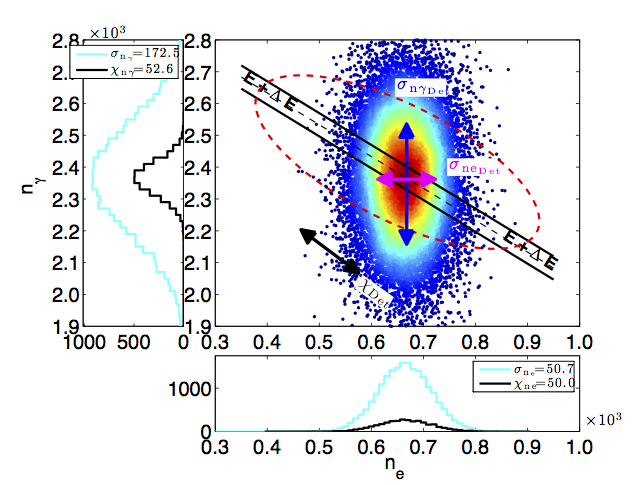
\includegraphics[width=160mm]{Chapter_Flucs/Figures/Ex_Plots/EX_Stat_Kr_.png}
\caption{A simulated \KrCal source with detector resolution and no recombination fluctuations. The solid black line represents constant energy about the center. The region between the black dashed lines represents a bin width of $\rm \Delta_E$ =1 and is where we make a cut. The events that fall between the black dashed lines are projected onto the $\rm n_\gamma$ and $\rm n_e$ axes. The observed variance in light and charge are shows on the labels with and without the energy cut, as $\rm \chi$ and $\rm sigma$ respectively. The energy cut has swept out a component of variance $\chi_Det$ that is shared between the light and charge channels. Note, $\chi_Det$ is about equal to the resolution of the best channel, $\rm \sigma_{n_{\gamma_{Det}}}$. }
\label{fig:Kr_ex_R}
\end{figure}
\renewcommand{\baselinestretch}{2}
\small\normalsize


\noindent In the example pictured in figure \ref {fig:Kr_ex_R} we find that the energy cut leaves a reduced statistical component to be projected onto $\rm n_\gamma$ and $\rm n_e$. The reduction in variance projected onto $\rm n_\gamma$ is large however, this is expected as only a small portion of $\rm n_\gamma$ is included with the energy cut. From the examples in figure \ref{fig:Kr_ex_R} and \ref{fig:Kr_ex_Stat} we can now visualize the effect of an energy cut on the light ($\rm n_\gamma$) and charge signals ($\rm n_e$). The slice contains those events which fluctuated about the line of constant energy thus, automatically including all recombination fluctuations along with reduced component from detector resolution.

To solve for the value of  $\rm \chi_{stat}$ we write the detector-resolution fluctuations $\rm \sigma_{n_{\gamma_{Det}}}$ and $\rm \sigma_{n_{e_{Det}}}$ as a function of combined energy in number quanta.

\begin{equation}
\rm n_q= E/W = n_\gamma + n_e
\label{eq:n_Q}
\end{equation}

\noindent where $\rm n_q$ is the number of quanta (photons + electrons), E is energy in keV, and W=0.0137 $pm$ 0.001 quanta/keV. Next, consider the the slope induced by the statistical variance of $\rm \sigma_{n_{\gamma_{Det}}}$ and $\rm \sigma_{n_{e_{Det}}}$ as a function quanta $\rm n_q$. The slope between $\rm n_\gamma$ with respect to energy $\rm n_q$ is simply the variance in $\rm n_\gamma$ over the variance in $\rm n_q$, and the same for $\rm n_e$. The result for the slope M considering a detector with resolution $\rm \sigma_{n_{\gamma_{Det}}}$ and $\rm \sigma_{n_{e_{Det}}}$ is,

\begin{equation}
\begin{split}
\rm M = tan(\theta_{n_{\gamma_{Det}}})=\frac{\sigma_{n_{\gamma_{Det}}}^2}{\sigma_{n_{\gamma_{Det}}}^2+ \sigma_{n_{\gamma_{Det}}}^2} \\
\rm 1-M = tan(\theta_{n_{e_{Det}}})=\frac{\sigma_{n_{e_{Det}}}^2}{\sigma_{n_{\gamma_{Det}}}^2+ \sigma_{n_{\gamma_{Det}}}^2} 
\label{eq:Angle}
\end{split}
\end{equation}

\noindent where M is the slope between $\rm n_\gamma$ as a function of $\rm n_q$ assuming a linear approximation, which is natural considering \ref{eq:n_Q}. The slope M can also be thought of as tan($\rm \theta$) where $\rm \theta$ is the angle between $\rm n_\gamma$ and $\rm n_q$, ranging from 0 to $\pi$/4. Once M is defined, the angle between $\rm n_e$ and $\rm n_q$ is the complementary slope (1-M). Recalling that $\rm n_\gamma$ + $\rm n_e$ sum to $\rm n_q$ by definition, in equation \ref{eq:n_Q}. The statistical distribution of $\rm n_gamma$ and $\rm n_e$ with respect to quanta (or E/W) can now be expressed interns of the slope M.

\begin{equation}
\begin{split}
\rm n_\gamma = M n_q \\
\rm n_e = (1-M) n_q \\
\label{eq:N_q_M}
\end{split}
\end{equation}

\noindent with equation \ref{eq:N_q_M} we now solve for a small variation in $\rm n_q$ (along a line of constant energy) induced by small fluctuations in $\rm n_\gamma$ and $n_e$.

\begin{multline}\\
\delta n_q = \frac{\partial n_\gamma}{\partial n_q} \delta n_q \bigg|_{n_{\gamma}} + \frac{\partial n_e}{\partial n_q} \delta n_q \bigg|_{n_{e}} \\
\delta n_q = \frac{\partial (n_q-n_e)}{\partial n_q} \delta n_e + \frac{\partial (n_q-n_\gamma)}{\partial n_q} \delta n_\gamma \\
\delta n_q = \bigg[\cancelto{\tiny{1}}{\frac{\partial n_q}{\partial n_q}}-\cancelto{\tiny{(1-M)}}{\frac{\partial n_e}{\partial n_q}}\bigg] \delta n_e + \bigg[\cancelto{\tiny{1}}{\frac{\partial n_q}{\partial n_q}}-\cancelto{\tiny{M}}{\frac{\partial n_\gamma}{\partial n_q}}\bigg] \delta n_\gamma  \\
\delta n_q = (M) \delta n_e + (1-M) \delta n_\gamma \\
\label{eq:Chi_Det}
\end{multline}

\noindent using the result from equation \ref{eq:Chi_Det} the variance along an infinitely thin line of constant energy induced by statistical fluctuations is

\begin{equation}
\rm \chi_{Det}^2= Var(\delta n_q) = M^2\sigma_{n_{e_{Det}}}^2 + (1-M)^2\sigma_{n_{\gamma_{Det}}}^2
\label{eq:SigCE}
\end{equation}

\noindent where the cross term $\rm \delta n_\gamma \delta n_e$ has been dropped as the statistical variance from detector resolution ($\rm \sigma_{n_{\gamma_{Det}}}^2$ and $\rm \sigma_{n_{n_{Det}}}^2$) are uncorrelated. Given equation \ref{eq:SigCE}, we have a method for determining the amount of statistical variance that will be included with the recombination fluctuations when we cut events along contours of constant energy. %(Note, an identical result to \ref{eq:SigCE} is reached when discarding the slope and dealing in centroid subtracted units (Patrick's thesis)).
 
%Patrick's derivation%%%%%%
\begin{comment}
\begin{multline}\\
\delta[\Delta n_e] = \delta[n_e] - \delta\left[\left<n_e\right>_{n_e+n_\gamma}\right]  \\
= \cancelto{1}{\frac{dn_e}{dn_e}} \delta[n_e] + \cancelto{0}{\frac{dn_e}{dn_\gamma}} \delta[n_\gamma] - \delta \left[\left<n_e\right>_{n_e+n_\gamma}\right] \\
= \delta[n_e] - \frac{d \left<n_e\right> }{d(n_e+n_\gamma)} \frac{d(n_e+n_\gamma)}{dn_e} \delta[n_e] - \frac{d\left<n_e\right>}{d(n_e+n_\gamma)} \frac{d(n_e+n_\gamma)}{dn_\gamma} \delta[n_\gamma] \\
\delta[\Delta n_e] = \delta[n_e] - \left(\delta[n_\gamma] + \delta[n_e]\right) \frac{d\left<n_e+n_\gamma\right>}{d\left(n_e+n_\gamma\right)} \\
\delta[\Delta n_e] = (M)\delta[n_e] - (1-M) \delta[n_\gamma] \\
\chi_{Det}^2 = Var(\Delta n_e) = (M)^2\delta^2[n_e] + (1-M)^2\delta^2[n_\gamma]-2M(1-M) \cancelto{0}{\delta[n_e]\delta[n_\gamma]} \\
\label{eq:Centroid}
\end{multline}
\end{comment}
%%%%%%%%%%%%%%%%

Let's briefly consider the implication of equation \ref{eq:SigCE}. For the case of $\rm \sigma_{n_{e_{Det}}}^2 = \sigma_{n_{\gamma_{Det}}}^2$, M=0.5, resulting in $\rm \sigma_{n_{e_{Det}}}^2=\sigma_{n_{\gamma_{Det}}}^2= \chi_{Det}^2$. This case can be thought of as sweeping out equal variance from the statistical population which would for a circle as illustrated in Figure \ref{fig:Recomb}. For the case of $\rm \sigma_{n_{e_{Det}}}^2 \neq \sigma_{n_{\gamma_{Det}}}^2$ the observed statistical variance in a slice of combined energy will become less than the variance of the best channel. Specifically for the LUX detector the implication of equation \ref{eq:SigCE} is that the statistical variance measured in a slice of combined energy will collapse to less than that of the S2 statistical uncertainty, as bin width $\rm \Delta_E$ goes to zero.


To complete the treatment of binned energy in this section we now add the final piece to the observed statistical variance, the contribution from the bin width $\rm \Delta_E$. The residual variance arrises from rotating the population of 2D gaussian about the bin center, the rotation having a slope of M or (1-M) as given in equation \ref{eq:Angle}. Note, the residual term from the slope can also be removed by centroid subtraction of the photons and electrons vs. energy as discussed later in section \ref{sec:Centroid}, in that case we are only left with $\chi_{Det}^2$ shared between the two channels.


\begin{equation}
\begin{split}
\rm \chi_{n_{\gamma_{Det}}}^2= \chi_{Det}^2 + \frac{(MW\Delta_E)^2}{12}\\
\rm \chi_{n_{e_{Det}}}^2= \chi_{Det}^2 + \frac{((1-M)W\Delta_E)^2}{12}\\
\label{eq:SigCE_2}
\end{split}
\end{equation}



Were $\chi^2$ is defined in \ref{eq:SigCE}, M is given in equation \ref{eq:Angle}, W is the work function in [quanta/keV], $\rm \Delta_E$ is a bin of energy keV, the normalization of 12 arrises from the second moment of a rotated line about its center. The total observed variance, $\rm \chi^2$, in the number of photons and electrons considering a bin of combined energy can now be determined transforming equation \ref{eq:SigR} to \ref{eq:Sig_total_CE}.

%%.... this equation holds for the standard deviation of a uniform distribution
 
\begin{equation}
\begin{split}
\rm \chi_{n_\gamma}^2 = \sigma_{n_{ex}}^2 + n_iF(r)^2 + \sigma_{r}^2 n_i^2 + \chi_{n_{\gamma_{Det}}}^2 \\
\rm \chi_{n_e}^2  = n_iF(1-r)^2 + \sigma_{r}^2 n_i^2 + \chi_{n_{e_{Det}}}^2
\label{eq:Sig_total_CE}
\end{split}
\end{equation}


In equation \ref{eq:Sig_total_CE} we have defined the observed standard deviation in units of quanta $\rm \chi$ for $\rm n_\gamma, n_e$ when working with bins of combined energy. In the limit that F, $\rm \sigma_{n_{ex}}^2$ and $\rm \Delta_E$ go to zero the observed variance in number of photons and electrons ($\rm \chi_{n_\gamma}$ and $\rm \chi_{n_e}$) are related to the size of recombination fluctuations in a given combined energy bin, equation \ref{eq:SigR_CE_lim}. Where $\rm \sigma_R$ is in units of quanta, $\rm \sigma_R = n_i\sigma_r$.

\begin{equation}
\begin{split}
\rm \sigma_{R_\gamma}^2 = \chi_{n_\gamma}^2 - \chi_{n_{\gamma_{Det}}}^2  \\
\rm \sigma_{R_e}^2 = \chi_{n_e}^2 - \chi_{n_{e_{Det}}}^2
\label{eq:SigR_CE_lim}
\end{split}
\end{equation}

We have arrived at the conclusion of this section, armed with equation \ref{eq:SigR_CE_lim} we now have two methods for determining the size of recombination fluctuations, $\rm\sigma_{R}^2$ where the subscript $\rm \gamma$ or e is used to represent the channel of quanta used for the calculation. Either the observed variance in the light and charge channel can be used to measure the size of recombination fluctuation in a bin of energy. Any asymmetry between the two methods has implications which are discussed in the following subsection.


\subsection{Measuring the Fano Factor in Bins of Energy}

There are three terms in equation \ref{eq:Sig_total_CE} that give rise to an asymmetry between the observed variance $\rm \sigma_{R_\gamma}^2$  and  $\rm \sigma_{R_e}^2$. The small difference in variance from the slope can be solved for exactly leaving just the Fano factor F and $\rm \sigma_{n_{ex}}^2$. By taking the difference of variance in the two channels component of recombination variance drops out leaving only the Fano factor and the variance in number of excitons, given in equation \ref{eq:Sig_total_CE}.

\begin{equation}
\rm \sigma_{R_\gamma}^2 - \sigma_{R_e}^2 = \sigma_{n_{ex}}^2 + n_iF(2r-1) 
\label{eq:Diff_X}
\end{equation}

F is the Fano factor, equation \ref{eq:Energy_2}, $\rm \sigma_{n_{ex}}^2$ is the variance of the number of excitons produced and r is the recombination fraction, equation \ref{eq:Quanta}. %The value of $\delta_{Det}$ is the small residual depending on the bin width $\rm \Delta_E$, equation \ref{eq:Residual_Stat}.
%\begin{equation}
%\rm \delta_{Det}= \sigma_{R_\gamma}^2 - \sigma_{R_e}^2 = \frac{(1-2M)(W\Delta_E)^2}{12}\\
%\label{eq:Residual_Stat}
%\end{equation}
Consider the case such that variance in the number of excitons $\rm \sigma_{n_{ex}}^2$ is much less than the contribution from the Fano factor. In such a regime we can solve for the Fano factor, potentially energy dependent, from equations \ref{eq:Diff_X}.

\begin{equation}
\rm F(E)=\frac{\sigma_{R_\gamma}^2 - \sigma_{R_e}^2}{n_i(2r-1)}
\begin{cases} \rm r \neq \frac{1}{2}\\
\end{cases}
\label{eq:Fano}
\end{equation}

There is an underlying subtlety to equation \ref{eq:Fano}. Remarkably, in the limit that $\rm \Delta_E$ goes to zero the Fano factor can be extracted with minimal knowledge of intrinsic detector statistical variance. Further, when the statistical variance of S1 and S2 are identical the value of M (equation \ref{eq:Residual_Stat}) will be 0.5. In that special case no knowledge of the statistical variance is needed to measure the Fano factor. 


When $ \rm r = \frac{1}{2}$ the coefficient in front of the Fano factor becomes zero in equation \ref{eq:Diff_X}. At this value an equal contribution from the Fano factor goes into the variance $\rm \chi^2$ of photons and electrons, allowing for the smaller value of $\rm \sigma_{ex}^2$ to be extracted. 

\begin{equation}
\rm \sigma_{n_{ex}}^2=\sigma_{R_\gamma}^2 - \sigma_{R_e}^2
\begin{cases} \rm r= \frac{1}{2} || \sigma_{n_{ex}}^2 > > n_iF(2r-1)\\
\end{cases}
\label{eq:SigmaEx}
\end{equation}

Equation \ref{eq:SigmaEx} is also valid in the case that $\rm \sigma_{n_{ex}}^2$ is much larger than the contribution form the Fano factor. This happens to be true when dealing with the time dependent light yield of $\rm ^{83m}Kr$, this topic will be explored in the next section.




\subsection{Application to $\rm^{83}Kr$}

Using the high stats Kr83 calibration data we can validate the method for working in a bin of energy since the exact solution for recombination and detector fluctuations can be measured, as outlined in section \ref{sec:flucs_mono} and \ref{sec:flucs_mono_bins}. Once the fluctuations from detector resolution are measured in the light and charge channel (S1 and S2 signals), the asymmetry between the two channels can be used to calculate the Fano factor (equation \ref{eq:Sig_total_CE} ). The asymmetry in fluctuations in the light and charge channel arrises from the Fano factor acting on ion production which is later amplified through the recombination fraction, as long as the recombination fraction does not equal 0.5. For the case of the $\rm ^{83m}Kr$ calibration the recombination fraction was 0.772 resulting in recombination fluctuations of 3 to 4 more quanta in the light channel as compared to the charge channel, see table \ref{table:R_Kr}. Though the additional recombination fluctuation is small having ample statistics the Fano factor can be constrained. 
The errors in the measurement were derived from simulated Kr data sets of 400,000 events with the Fano factor turned off, using 100 trials. First, recombination fluctuations were turned off and only fluctuations from detector resolution as calculated in section \ref{sec:flucs_mono} were used, see Table \ref{table:Simulated_Sigmas_R_0}. It was found that the error of the difference in recombination fluctuation from the light and charge channel ($\rm sigma_{R_{\gamma}}^2$ and $\sigma_{R_{e}}^2 $) along with the error in ion production and recombination fraction were enough to constrain the Fano factor to 0.001-0.003. Next, the value of recombination was set slightly higher than the actual value of 82 to 100 quanta and the trials were repeated, see table \ref{table:Simulated_Sigmas_R_100}. With the addition of recombination fluctuations to detector resolution fluctuations the error on measuring the Fano factor grew to 0.002-0.009, with smaller bin sizes ($\rm\Delta E$ around the center leading to the smallest error as seen from equation \ref{eq:SigCE_2}.


\begin{table}[h!]
\begin{center}
\begin{tabular}{|c|c|c|c|c|c|}
\hline
$\rm \Delta_E$ keV & Count & $\rm \sigma (\sigma_{R_{\gamma}}^2 ) $ & $\rm \sigma (\sigma_{R_{e}}^2 )$  & $\rm \sigma (\sigma_{R_{\gamma}}^2 - \sigma_{R_{e}}^2 ) $ & $\rm \sigma F$ \\ \hline
0.025 	& 1528 		&77.8		& 77.9	  	& 1.3	&	0.0008 \\ \hline
0.05 	& 3063 		&54.4		& 54.6	  	& 1.8	&	0.0012 \\ \hline
0.1 		& 6128  	&36.4		& 36.6		& 2.6	&	0.0016  \\ \hline
0.2 		& 12242  	&23.7		& 23.8	 	& 3.7	&	0.0023 \\ \hline
0.25 	& 15290 	&22.9		& 22.9		& 4.0 	&	0.0026 \\ \hline
0.5		& 30528 	&17.5		& 17.5 		& 5.2	& 	0.0033	 \\ \hline
\end{tabular}
\caption{Values for the standard deviation of the observed value of $\rm \sigma_R^2$ from $\rm n_\gamma$ and $\rm n_e$ along with the standard deviation of the difference, for a simulated $\rm^{83m}Kr$ decay with recombination set to zero.  Note, since the two methods for determining $\rm \sigma_R^2$  are correlated the standard deviation of the measured difference is small leading to an improved error when calculating the Fano factor or $\rm \sigma_{n_{ex}}^2$.}
\label{table:Simulated_Sigmas_R_0}
\end{center}
\end{table}

\begin{table}[h!]
\begin{center}
\tabcolsep=0.11cm
\begin{tabular}{|c|c|c|c|c|c|}
\hline
$\rm \Delta_E$ keV & Count & $\rm \sigma (\sigma_{R_{\gamma}}^2 ) $ & $\rm \sigma (\sigma_{R_{e}}^2 )$  & $\rm \sigma (\sigma_{R_{\gamma}}^2 - \sigma_{R_{e}}^2 ) $ & $\rm \sigma F$ \\ \hline
0.025 	& 1523		&498		& 498	  	& 3.2	&	 0.0020\\ \hline
0.05 	& 3056 		&347		& 347	  	& 4.1	&	 0.0026\\ \hline
0.1 		& 6118  	&237		& 237		& 5.3	&	 0.0033\\ \hline
0.2 		& 12225  	&171		& 171	 	& 8.6	&	 0.0054\\ \hline
0.25 	& 15285 	&149		& 148		& 9.5 	&	 0.0060\\ \hline
0.5		& 30514 	&101		& 99.4  		&14.3	&	 0.0090 \\ \hline
\end{tabular}
\caption{Values for the standard deviation of the observed value of $\rm \sigma_R^2$ from $\rm n_\gamma$ and $\rm n_e$ along with the standard deviation of the difference, for a simulated $\rm^{83m}Kr$ decay with recombination set to 100 quanta.  Note, since the two methods for determining $\rm \sigma_R^2$  are correlated the standard deviation of the measured difference is small leading to an improved error when calculating the Fano factor or $\rm \sigma_{n_{ex}}^2$.}
\label{table:Simulated_Sigmas_R_100}
\end{center}
\end{table}


The results of the high stats calibration data are shown in table \ref{table:R_Kr}, containing 400k events in the fiducial volume of the detector. Using equation \ref{eq:SigR_CE_lim} we find good agreement between the method described in equation \ref{eq:Dahl} and the recombination fluctuation calculated from the charge channel ($\rm \sigma_{R_\gamma}$ and $\rm \sigma_{R_e}$).  The accuracy helps us build confidence that the statistical components of the detector are modeled well enough to measure recombination fluctuation to within 3\%. Further, the ability to see the asymmetry in recombination fluctuations between the light and charge channel demonstrates the power of using binned combined energy (section \ref{sec:flucs_mono_bins}). Any observed difference between the two channels  can only be from either the Fano factor or spread in exiton production, but we assume the fluctuations in exiton production are much less than fluctuations in ion production. The Fano factor is derived from equations \ref{eq:Fano} and the uncertainty was determined from simulations. The total fluctuation as number of quanta is listed in the rightmost column. The Fano factor manifests itself as an asymmetry between fluctuations in the light and charge channel as given in equation \ref{eq:Sig_total_CE}, the recombination fraction was found to be r= 0.772 and the average number of ions produced per decay was $\rm n_i=2900$. 
Having demonstrated the method for a mono energetic calibration source the next step will be to apply the method on the continuous beta spectrum of the tritium data.



\begin{table}[h!]
\begin{center}
\footnotesize
\tabcolsep=0.11cm
\begin{tabular}{|c||c|c|c|c|c|c|}
\hline
$\rm \sigma_R$ \ref{eq:Dahl} & $\rm \Delta_E$ & Count & $\rm \sigma_{R_\gamma}=\sqrt{\chi_{n_{\gamma}}^2-\chi_{n_{\gamma_{Det}}}^2}$ & $\rm \sigma_{R_e}= \sqrt{\chi_{n_{e}}^2-\chi_{n_{e_{Det}}}^2}$  & $\rm F=\frac{\sigma_{R_{\gamma}}^2-\sigma_{R_e}^2}{n_i(2r-1) }$ &$\rm \sqrt{Fn_i}$ \\ 
(Quanta) & (keV) & & (Quanta) & (Quanta) & (Quanta) & (Quanta)\\ \hline
82.4 $\pm$ 4.0		& 0.025		& 1518 		& 87.2 $\pm$ 2.9	 	&	87.1 $\pm$ 2.9	& 0.010 $\pm$ 0.002     & 5.8 $\pm$ 0.5 \\ \hline
					& 0.05 		& 3124 		& 85.0 $\pm$ 2.0	 	&	84.9 $\pm$ 2.0	& 0.005 $\pm$ 0.003	& 3.8 $\pm$ 1.1 \\ \hline
					& 0.1 		& 6269  	& 87.8 $\pm$ 1.3		& 	87.6 $\pm$ 1.3	& 0.023 $\pm$ 0.003	& 8.1 $\pm$ 0.5	 \\ \hline
					& 0.2 		&12508  	& 90.0 $\pm$ 1.0  		& 	89.7 $\pm$ 1.0	& 0.021 $\pm$ 0.005	& 7.8 $\pm$ 0.9	 \\ \hline
					& 0.25 		&15557 	& 88.5 $\pm$ 0.8		&	88.3 $\pm$ 0.8  & 0.013 $\pm$ 0.006	& 6.1 $\pm$ 1.3	 \\ \hline
					& 0.5		& 30826 	& 87.0  $\pm$ 0.6		&	86.7 $\pm$ 0.6	& 0.027	$\pm$  0.009 	& 8.8 $\pm$ 2.2	\\ \hline
\end{tabular}
\caption{Values for the standard deviation of the observed value of $\rm \sigma_R^2$ from $\rm n_\gamma$ and $\rm n_e$ along with the standard deviation of the difference, for a $\rm^{83m}Kr$ data set with 400k events in the fiducial volume. The Fano factor is derived from equations \ref{eq:Fano} and the uncertainty was determined from simulations. The total fluctuation as number of quanta is listed in the rightmost column. The Fano factor manifests itself as an asymmetry between fluctuations in the light and charge channel as given in equation \ref{eq:Sig_total_CE}, with a recombination fraction of 0.772 and $\rm n_i = 2900$. }% add note about excitons
\label{table:R_Kr}
\end{center}
\end{table}


\subsection{Application to Simulated Tritium Data (any continuous spectrum)}

%ref Partrick
%This will be demonstrated later (or maybe show it in the simulation)
Adapting the equation of the previous section to continuous energy spectra requires that the centriod of a continue spectrum be subtracted off so that the variance from the light yield or charge yield vs. energy is removed. After applying the Smearing Model of Section 4 we apply the method described in this section to extract recombination fluctuations form the tritium data.

In this subsection we test method outlined in section \ref{sec:flucs_mono_bins} for dealing in bins of combined energy specifically applied to the tritium beta spectrum, but the method outlined can be used for any continue spectrum. To first order the treatment of the continuous spectrum is identical to that outlined for the mono energetic source as outlined previously in subsection \ref{sec:flucs_mono_bins}. Figure \ref{fig:T_Stat} illustrates a tritium beta spectrum convolved with detector resolution similar to that measured for the LUX detector, the figure is analogous to Figure \ref{fig:Recomb}. As the bin size around a value of combined energy is squeezed to zero the statistical variance in the number of photons and electrons converge, the value is given by equation \ref{eq:SigCE_2}. Whereas, regardless of bin size recombination fluctuations remain since they move along lines of constant energy. In order to adapt the methodology developed for a mono energetic source to a continuous energy spectra requires that the centriod of the light and charge yield be subtracted off. The slope in the light and charge channels from the fundamental yield  induce a further variance on top of $\rm \chi_{Det}$ from the population in an energy bin being tilted as demonstrated in figure \ref{fig:SIM_LYQY}. For the purposes of this study, we find it sufficient to fit a quadratic form to the centroid of the entire population and subtract off the local slope from the measured variance. An analogous methods for centriod subtraction to extract recombination fluctuations are described in detail in [Patrick's Thesis].



\begin{figure}[h!]\centering
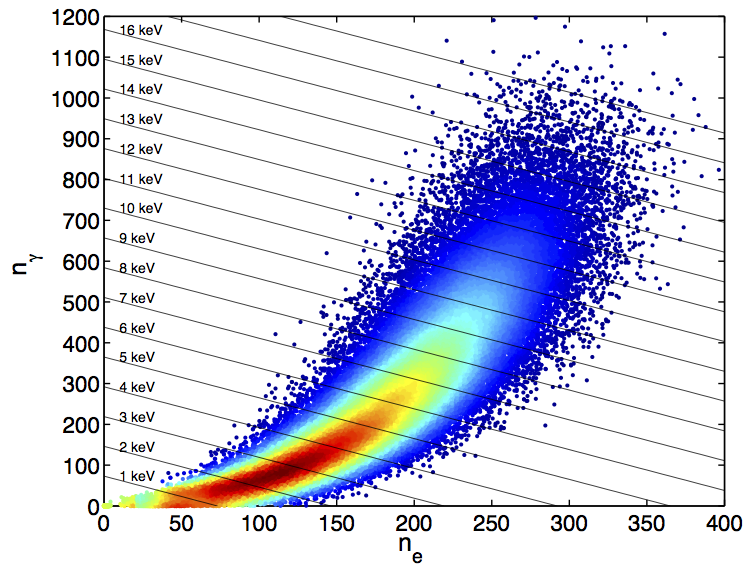
\includegraphics[width=130mm]{Chapter_Flucs/Figures/EX_T_Fano.png}
\caption{Illustration of statistical variance for the tritium beta spectrum, recombination fluctuations are set to 0. This plot is analogous to Figure \ref{fig:Recomb} which illustrates the case for the mono energetic $\rm ^{83m}Kr$ decay. Recombination fluctuation move along lines of constant energy, S1 statistical fluctuation move vertically and S2 statistical fluctuations move horizontally. }
\label{fig:T_Stat}
\end{figure}

\begin{figure}[h!]\centering
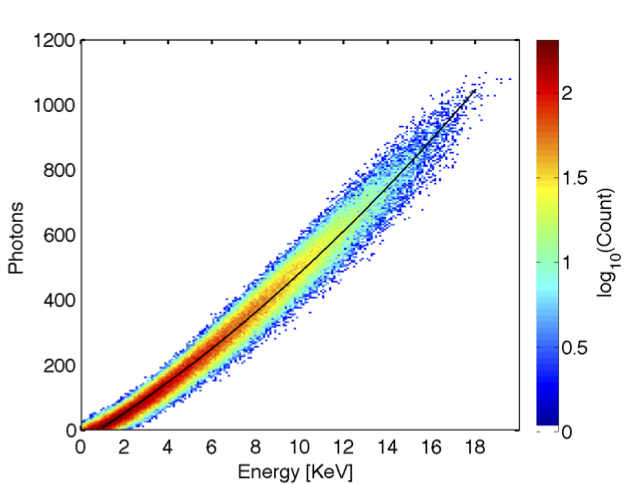
\includegraphics[width=70mm]{Chapter_Flucs/Figures/T_SIM/n_photon_180_.png}
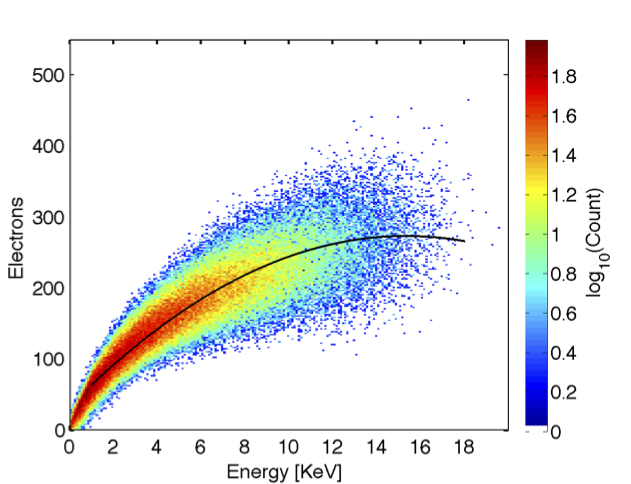
\includegraphics[width=70mm]{Chapter_Flucs/Figures/T_SIM/n_e_180_.png}
\caption{Light yield (left) and Charge yield (right) of a simulated tritium spectrum, with the fit to the centroid show in black. The variance in number of photon and electrons per energy bin is used to extract recombination fluctuations.}
\label{fig:SIM_LYQY}
\end{figure}

%Add centriod subtracted equation. Explain that even if S1, S2 Det are off we can do as good as the best channel (S2) due to X_Det. As long as SigR is greater, since they add in quadrature.


\subsection{Centriod Subtraction}
\label{sec:Centroid}
For the case of a continuous source we expand upon the result from section \ref{sec:flucs_mono_bins} where the additional variance from detector resolution was calculated per energy bin as $\rm \chi_{n_{\gamma_{Det}}}^2$ and $\rm \chi_{n_{e_{Det}}}^2$. When dealing with a continuous source we must subtract off the centroid of the number of photons and electron vs. energy to remove additional variance induced by the slope. What results is a common variance from detector resolution shared by both the charge and light channel in each bin of energy, defined as $\rm \chi_{Det}^2$ = $\rm \chi_{n_{\gamma_{Det}}}^2$ = $\rm \chi_{n_{e_{Det}}}^2$, equation \ref{eq:SigR_Cent}. The value of $\rm \chi_{Det}^2$ is derived in \ref{eq:Centroid} for a small variation in $\rm n_e$ around combined energy, and is identical to that found for the case of the mono energetic source in equation \ref{eq:SigCE}. This is analogous to saying that the centroid subtraction is removing the additional variance from the slope of light field and charge yield. The local slope of  $\rm n_e$ with respect to quanta ($\rm n_\gamma + n_e$) is (1-M), given in \ref{eq:Angle}. 
To demonstrate the effectiveness of the method we use the measured detector resolution along with a test recombination fluctuation and simulate a tritium spectrum. The result of extracting recombination is shown in figure \ref{fig:T_Var} for various energy bin widths. As long as the recombination is greater than $\rm \chi_{Det}$, which is being added in quadrature, the value of recombination can be determined to good precision using the method. The small deviation around the first and last bins is due to the spectral shape, a correction for spectral shape will be discussed in the next section and will improve the measurement of $\rm \sigma_R$. The analytic solution for extracting recombination given in equation \ref{eq:SigR_Cent} is sufficient to first order, we ignore second order corrections in this analysis. After correcting observables for the tritium beta spectral shape we will be ready to use the tools of this section to decouple detector resolution and measure recombination fluctuations from the tritium data

\begin{equation}
\begin{split}
\rm \sigma_{R_\gamma}^2 = \chi_{n_\gamma}^2 - \chi_{Det}^2  \\
\rm \sigma_{R_e}^2 = \chi_{n_e}^2 - \chi_{Det}^2 \\
\label{eq:SigR_Cent}
\end{split}
\end{equation}


\begin{multline}\\
\delta[\Delta n_e] = \delta[n_e] - \delta\left[\left<n_e\right>_{n_e+n_\gamma}\right]  \\
= \cancelto{1}{\frac{dn_e}{dn_e}} \delta[n_e] + \cancelto{0}{\frac{dn_e}{dn_\gamma}} \delta[n_\gamma] - \delta \left[\left<n_e\right>_{n_e+n_\gamma}\right] \\
= \delta[n_e] - \frac{d \left<n_e\right> }{d(n_e+n_\gamma)} \frac{d(n_e+n_\gamma)}{dn_e} \delta[n_e] - \frac{d\left<n_e\right>}{d(n_e+n_\gamma)} \frac{d(n_e+n_\gamma)}{dn_\gamma} \delta[n_\gamma] \\
\delta[\Delta n_e] = \delta[n_e] - \left(\delta[n_\gamma] + \delta[n_e]\right) \frac{d\left<n_e+n_\gamma\right>}{d\left(n_e+n_\gamma\right)} \\
\delta[\Delta n_e] = (M)\delta[n_e] - (1-M) \delta[n_\gamma] \\
\chi_{Det}^2 = Var(\Delta n_e) = (M)^2\delta^2[n_e] + (1-M)^2\delta^2[n_\gamma]-2M(1-M) \cancelto{0}{\delta[n_e]\delta[n_\gamma]} \\
\label{eq:Centroid}
\end{multline}


\begin{figure}[h!]\centering
 
\subcaptionbox{\label{fig:1a}}{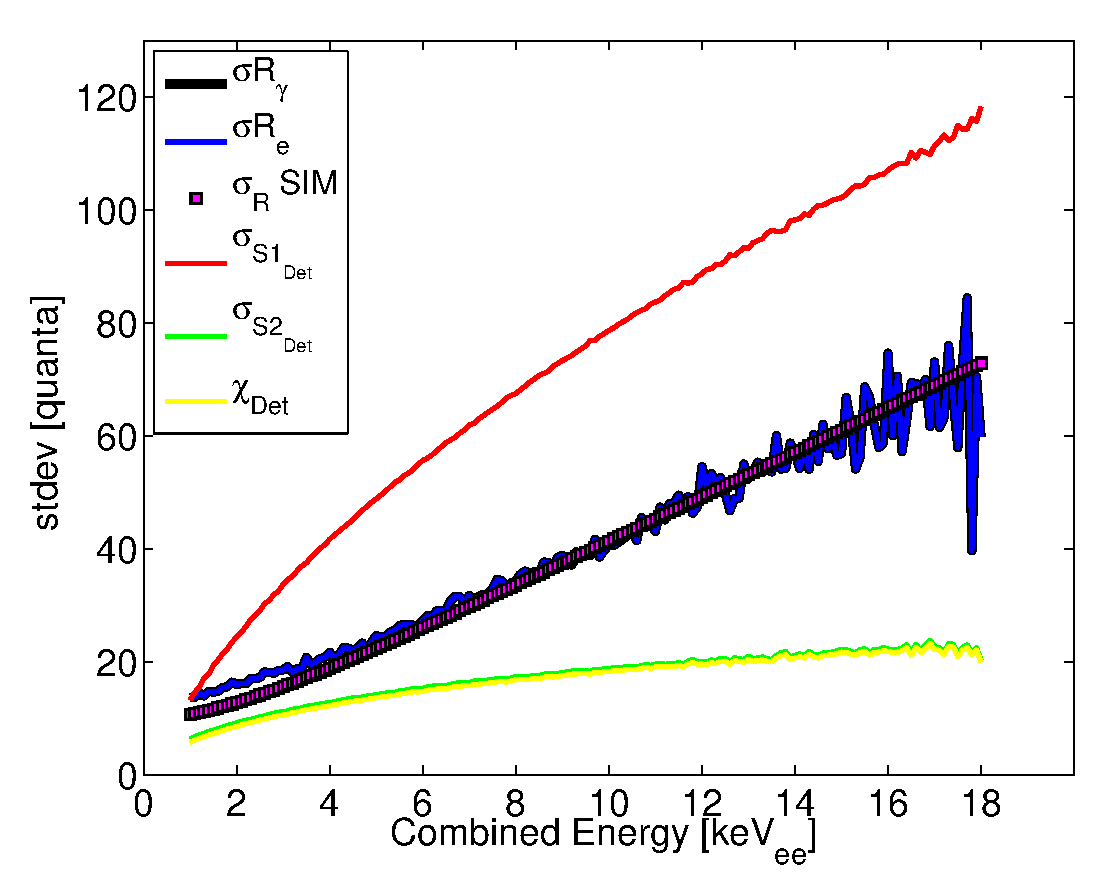
\includegraphics[width=70mm]{Chapter_Flucs/Figures/T_SIM/SIM_R_T_10.eps}}
\hfill
\subcaptionbox{\label{fig:1b}}{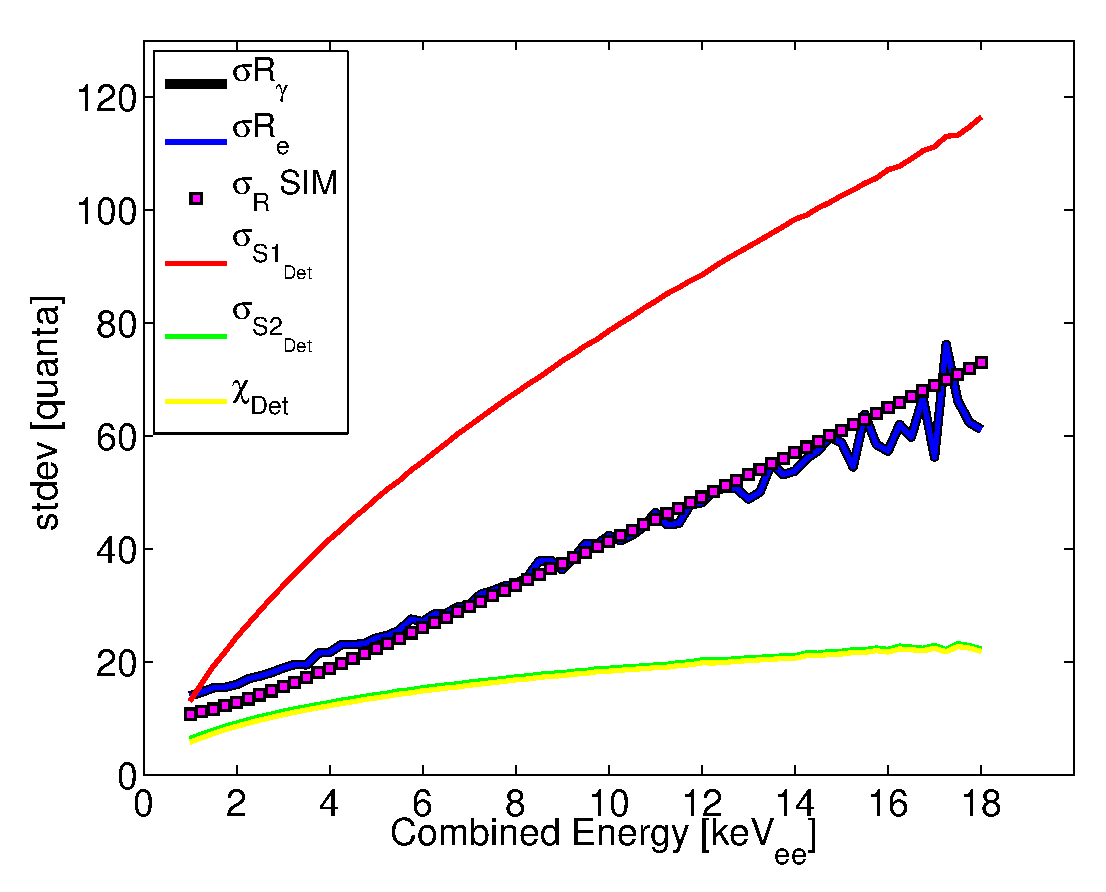
\includegraphics[width=70mm]{Chapter_Flucs/Figures/T_SIM/SIM_R_T_25.eps}}


\bigskip

\subcaptionbox{\label{fig:1c}}{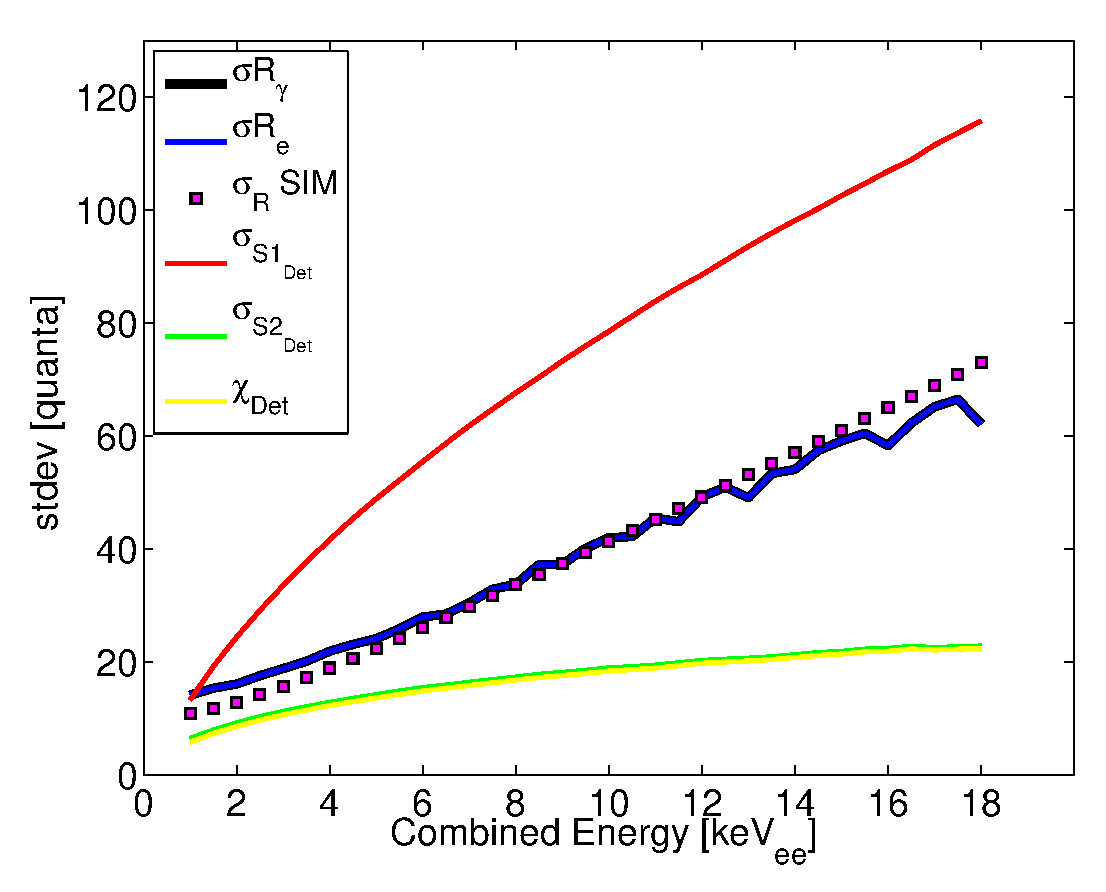
\includegraphics[width=70mm]{Chapter_Flucs/Figures/T_SIM/SIM_R_T_50.eps}}
\hfill
\subcaptionbox{\label{fig:1d}}{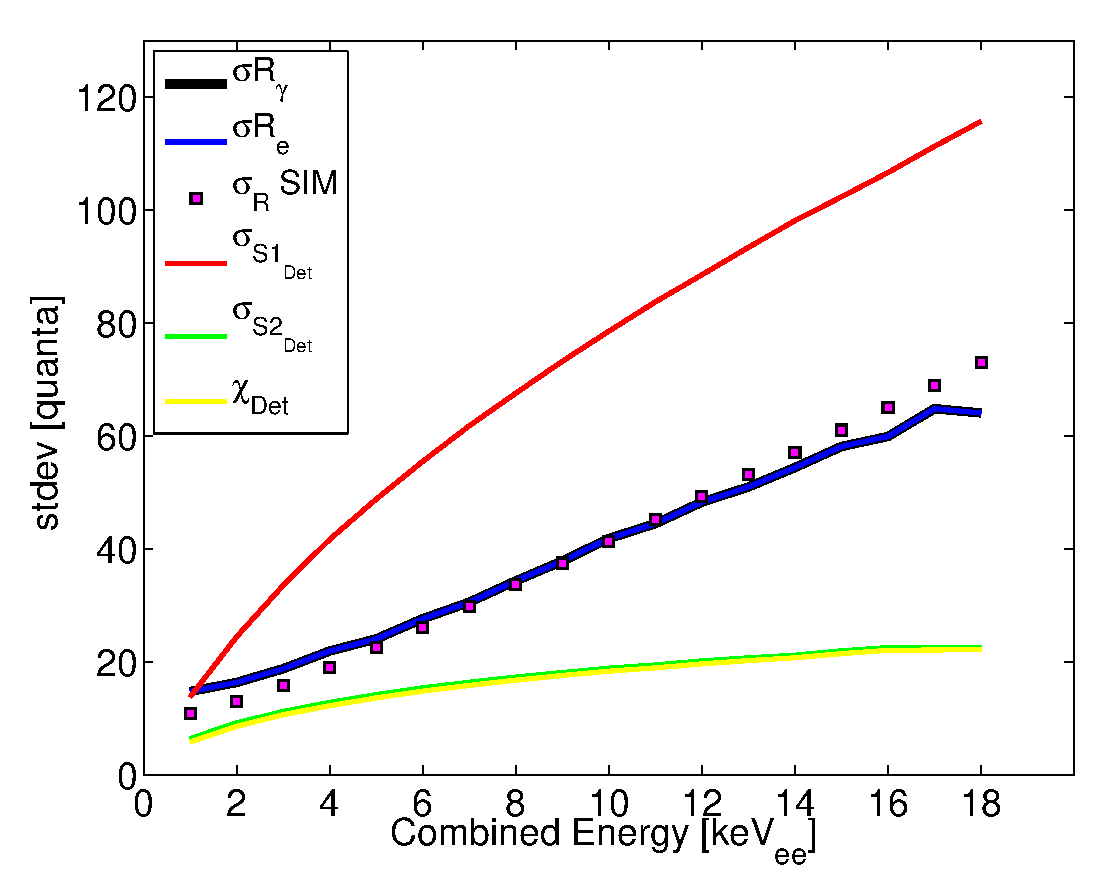
\includegraphics[width=70mm]{Chapter_Flucs/Figures/T_SIM/SIM_R_T_100.eps}}


\caption{Simulated tritium spectrum with the detector resolution of the LUX detector, $\rm \sigma_{S1_{Det}}$ and $\rm \sigma_{S2_{Det}}$, and an arbitrary recombination fluctuation $\rm \sigma_R$ (magenta). After centroid subtraction we apply the methodology described in the previous section to extract $\rm \sigma_R$ (black and blue) through the light and charge channel using our knowledge of detector resolution per each energy bin $\rm \chi_{Det}$ (green), $\rm S1_{Det}$ (red) and $\rm S2_{Det} $(yellow). The plots show cases for various bin widths in keV: a) $\rm \Delta E$ = 0.1 b) $\rm \Delta E$ = 0.25 c) $\rm \Delta E$ = 0.5 d) $\rm \Delta E$ = 1.   }
\label{fig:T_Var}
\end{figure}% Extracting Recombination variance vs. delta E for a simulated tritium spectrum. The smaller deltaE the smaller the effect of slope on the measurement, though it is found that subtracting off the centroid with a quadratic fit is sufficient.


\newpage


\section{Extracting Recombination Fluctuations from Tritium Calibration Data}
\label{sec:Recomb_Data}

In this section we apply the methods outlined in this chapter and use them to extract the recombination fluctuations vs. energy from the tritium data. The first step in this process was calibrate the energy scale solving for $\rm g_1$ and $\rm g_2$ as outlined in \ref{Ch:E_Scale_Cal}. Second, the S1 and S2 signals of the tritium calibration data were corrected for spectral shape as outlined previously in section \ref{sec:Smear} and discussed in more detail in \ref{Ch:LYQY}. Finally, having modeled and measured the statistical and instrumented variances for light collection of the LUX detector \ref{eq:SigDet} \ref{eq:SigStat} \ref{eq:SigInst} the component of detector resolution in each energy bin can be calculated $\rm \chi_{Det}^2$ \ref{eq:SigCE}, ref{eq:Angle}, {eq:Centroid}. For the remained of the thesis we will work in centroid subtracted space as detailed in equation {eq:Centroid}, the results are identical to working in non centroid subtracted space using a bin width correction of equation \ref{eq:SigR_CE_lim}, which is the equivalent of making a linear approximation to the local slope.  


Since the tritium beta spectrum is continuous the calibration data is divided into energy bins. In each energy bin the mean of S1 and $\rm S2_b$ is measured and converted to the mean number of photons and electrons using $\rm g_1$ and $\rm g_2$. Once that is known the variance from detector resolution in each bin can be determined, defined as $\rm \chi_{Det}^2$ \ref{eq:Centroid}, \ref{eq:SigCE}. We then measure the variance of both the fluctuations in the photon and electron channels using Gaussian fits to the distributions in each energy bin, defined as $\rm \chi^2$. The recombination variance and variance from detector resolution are two independent processes making the observed variance in each bin $\rm \chi^2$ a sum of $\rm \chi_{Det}^2$ and $\rm \sigma_R^2$. We measure the variance of both the light and channel $\rm \chi_{\gamma}^2$ and $\rm \chi_e^2$ and solve for $\rm \sigma_{R_\gamma}^2$ and $\rm \sigma_{R_e}^2$ where the subscripts $\rm \gamma$ and e denote the photon and electron channel respectively. Using this we find
\begin{equation}
\rm \sigma_R^2 = \sigma_{R_\gamma}^2 = \sigma_{R_e}^2 = \chi^2-\chi_{Det}^2
\end{equation}
\noindent the same result as outlined in \ref{eq:SigR_Cent}. The recombination fluctuation $\rm \sigma_R$ can be extracted from the tritium calibration data. The result of the tritium calibration is shown in figure \ref{fig:R_Flucs_Quanta} for both the 170 V/cm and 100 V/cm data. The 170 V/cm data had 140,000 tritium beta decays in the fiducial volume and the 100 V/cm data contained 4,500 events. 


%

\renewcommand{\baselinestretch}{1}
\small\normalsize
\begin{figure}[h!]\centering
 
\subcaptionbox{$\rm n_\gamma$, 170 V/cm \label{fig:5a}}{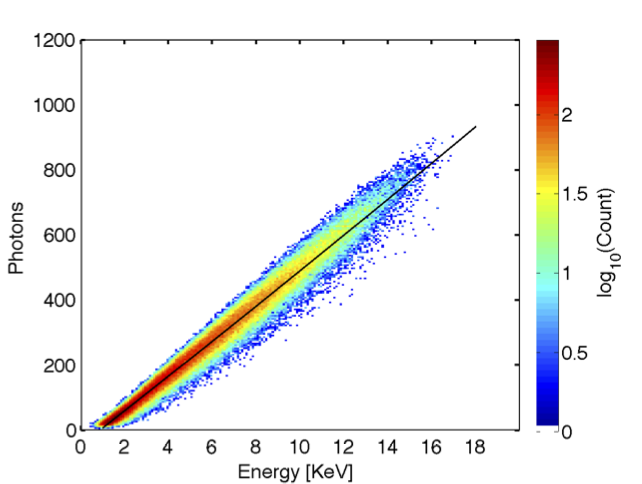
\includegraphics[width=75mm]{Chapter_Flucs/Figures/Quanta_Density/n_photon_iter1_180_.png}}
\hfill
\subcaptionbox{$\rm n_e$, 170 V/cm \label{fig:5b}}{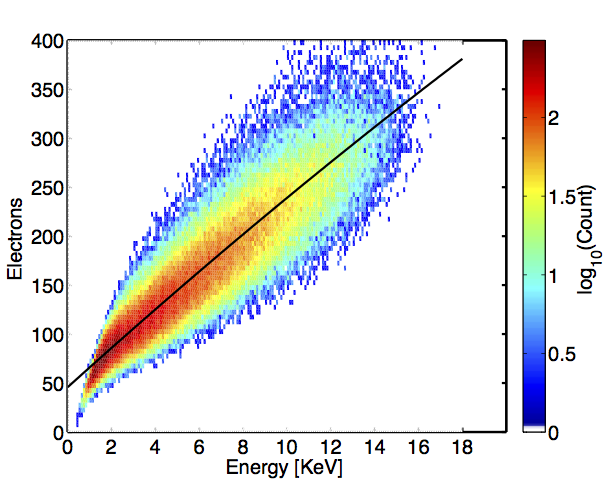
\includegraphics[width=73mm]{Chapter_Flucs/Figures/Quanta_Density/n_electron_iter1_180_.png}}

\bigskip

\subcaptionbox{$\rm n_\gamma$ 100 V/cm \label{fig:5c}}{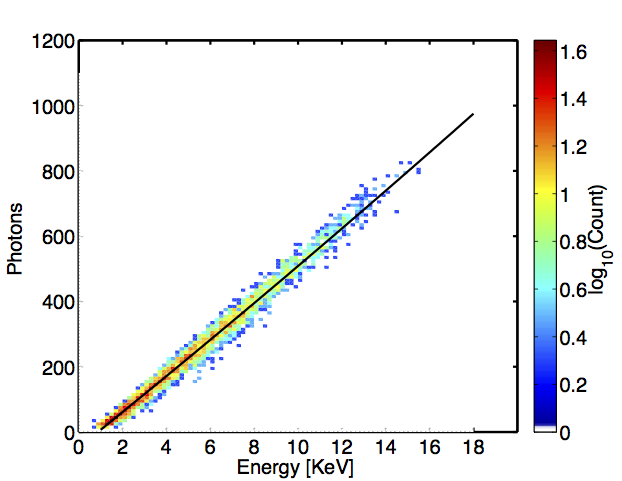
\includegraphics[width=75mm]{Chapter_Flucs/Figures/Quanta_Density/n_photon_100_iter1_180_Tritium_LY_QY_100_iter1.png}}
\hfill
\subcaptionbox{$\rm n_e$, 100 V/cm \label{fig:5c}}{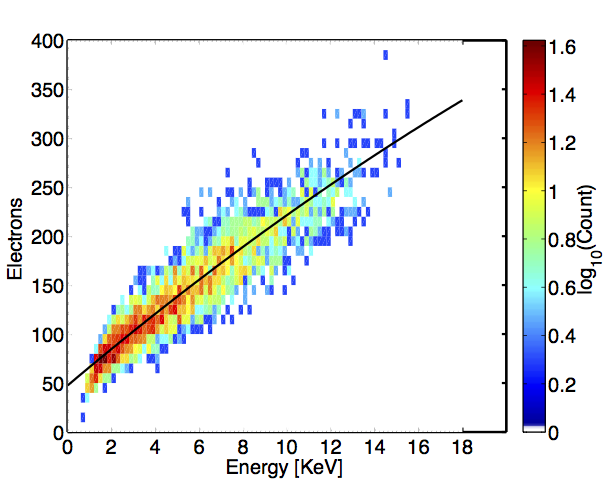
\includegraphics[width=73mm]{Chapter_Flucs/Figures/Quanta_Density/n_electron_100_iter1_180_Tritium_LY_QY_100_iter1.png}}

\caption{a: Density plot of number of photons vs. energy in keV using the tritium calibration data at 170 V/cm. b: Number of electrons vs. energy in keV using the tritium calibration data at 170 V/cm. c: Number of photons vs. energy in keV using the tritium calibration data at 100 V/cm. d: Number of electrons vs. energy in keV using the tritium calibration data at 100 V/cm. The data has been corrected for spectral shape. The black line indicates the quadratic fit to the centroid of the population. }
\label{fig:Raw_Quanta}
\end{figure}
\renewcommand{\baselinestretch}{2}
\small\normalsize


%
\renewcommand{\baselinestretch}{1}
\small\normalsize
\begin{figure}[h!]\centering
 
\subcaptionbox{$\rm \sigma_R$, 170 V/cm \label{fig:5a}}{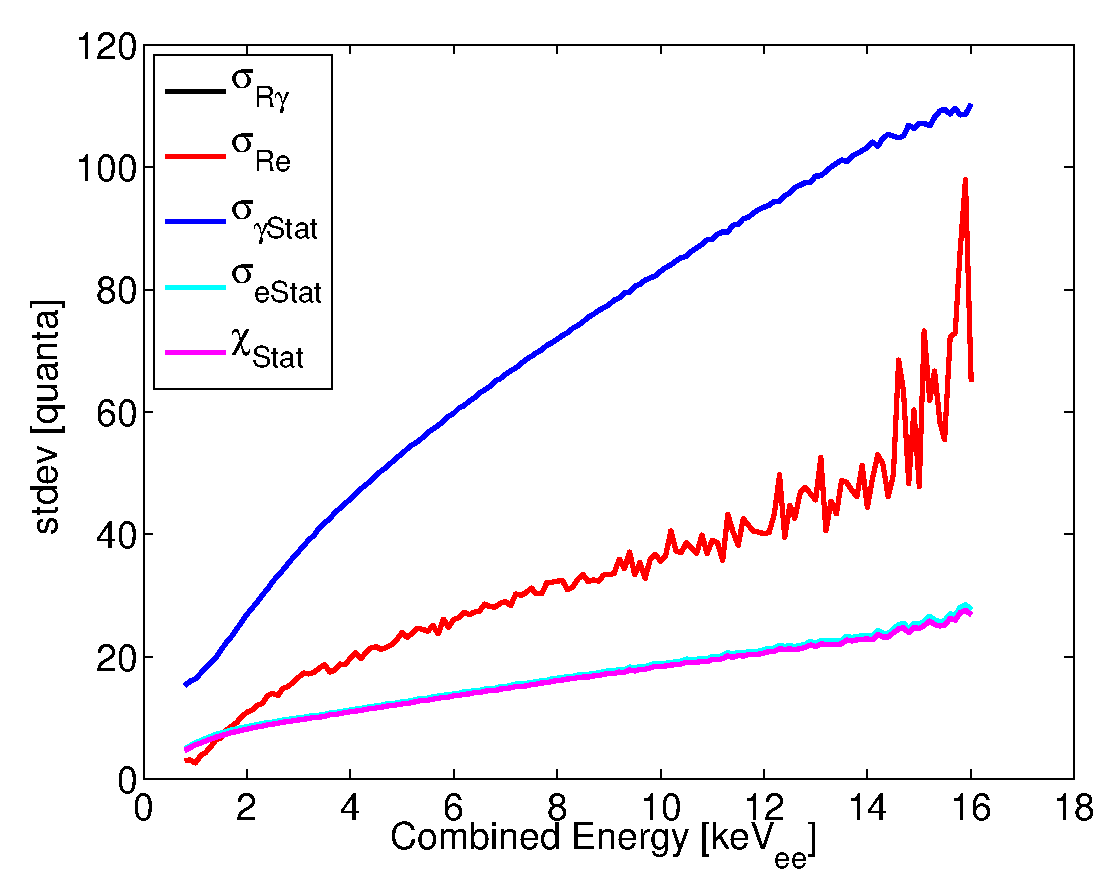
\includegraphics[width=75mm]{Chapter_Flucs/Figures/Iter1/std_fig_iter1LY_QY_iter1.eps}}
\hfill
\subcaptionbox{Quanta, 170 V/cm \label{fig:5b}}{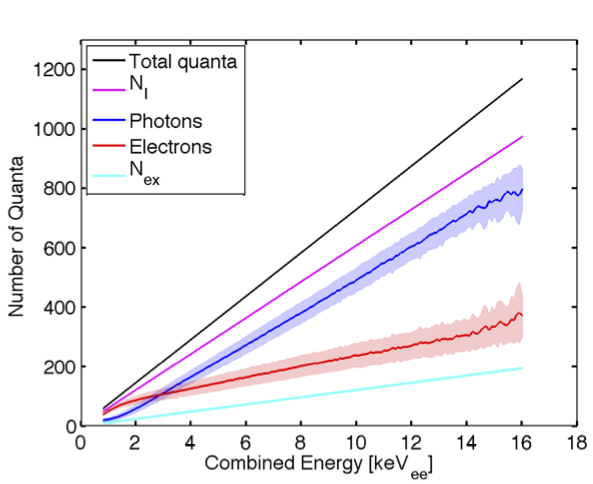
\includegraphics[width=73mm]{Chapter_Flucs/Figures/Iter1/quanta_inter1Tritium_LY_QY_iter1.png}}

\bigskip

\subcaptionbox{$\rm \sigma_R$, 100 V/cm \label{fig:5c}}{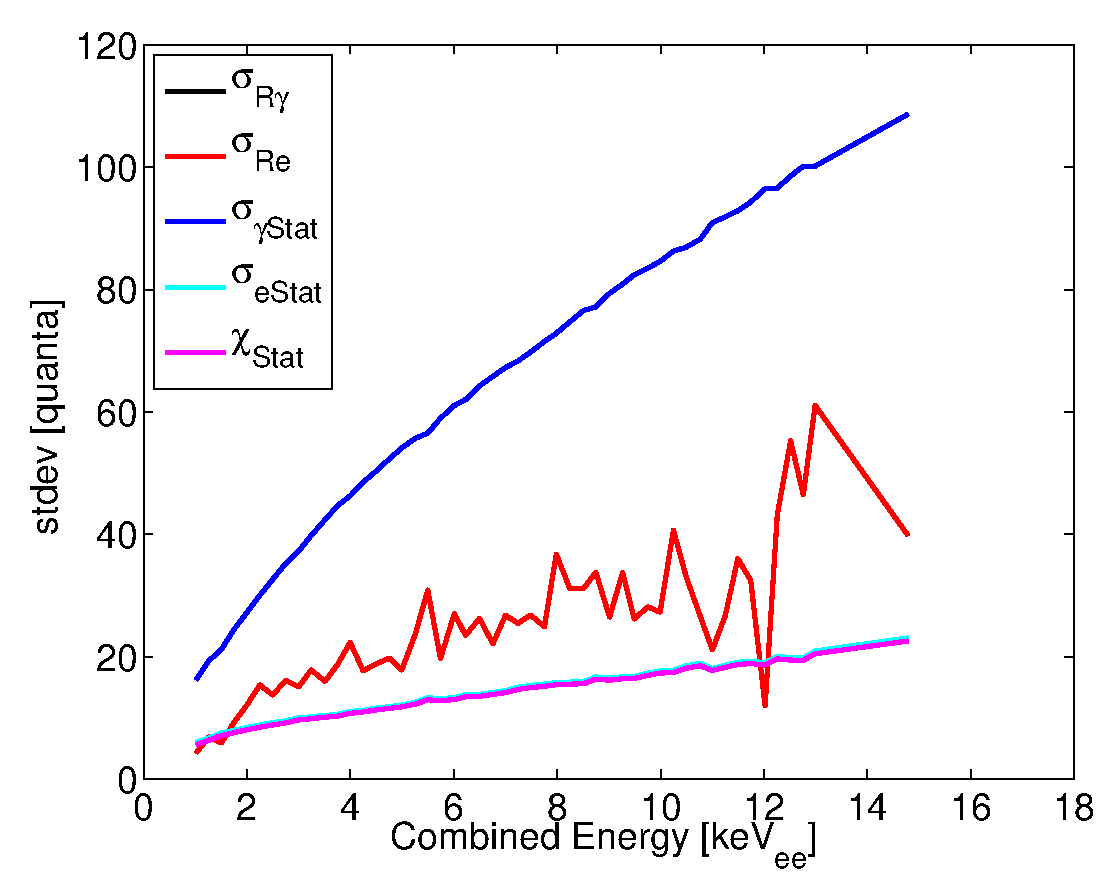
\includegraphics[width=75mm]{Chapter_Flucs/Figures/Iter1_100/std_fig_100_iter1Tritium_LY_QY_100_iter1.eps}}
\hfill
\subcaptionbox{Quanta, 100 V/cm \label{fig:5c}}{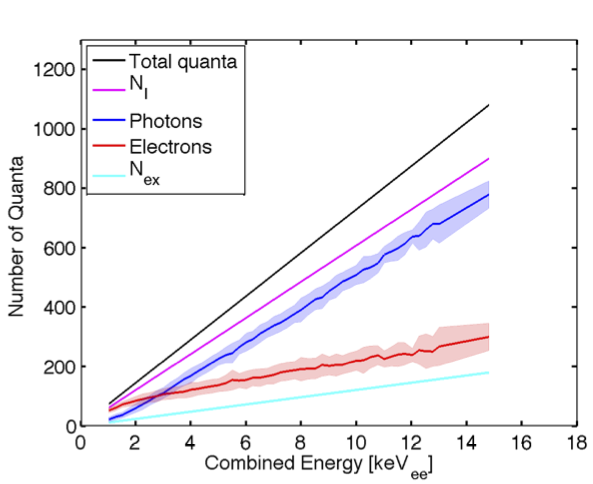
\includegraphics[width=73mm]{Chapter_Flucs/Figures/Iter1_100/quanta_100_iter1.png}}

\caption{The figures on the left in \ref{fig:R_Flucs_Quanta} (a: 170 V/cm, c: 100 V/cm) show the extracted recombination fluctuation $\rm \sigma_R$ from the light (black) and change (red) channel denoted with subscript $\gamma$ and e respectively, note they are identical. Also shown are the fluctuations in light collection $\rm \chi_{\gamma_{Det}}^2$ (blue), charge collection $\rm \chi_{e_{Det}}^2$ (cyan), and their manifestation as detector resolution in a combined energy bin as $\rm \chi_{Det}$ (magenta). The figures on the right in in \ref{fig:R_Flucs_Quanta} (b: 170 V/cm, d: 100 V/cm) show the mean and one sigma standard deviation of the measured number of photons (blue) and electrons (red). Also shown is the total quanta (in black) which is the sum of photons and electrons and the expected number of ions (magenta) and excitons (cyan) using $\rm \alpha$ = 0.20.}
\label{fig:R_Flucs_Quanta}
\end{figure}
\renewcommand{\baselinestretch}{2}
\small\normalsize

The figures on the left in \ref{fig:R_Flucs_Quanta} (a: 170 V/cm, c: 100 V/cm)  show the extracted recombination fluctuation $\rm \sigma_R$ from the light (black) and change (red) channel denoted with subscript $\gamma$ and e respectively, note they are identical. Also shown are the fluctuations in light collection $\rm \chi_{\gamma_{Det}}^2$ (blue), charge collection $\rm \chi_{e_{Det}}^2$ (cyan), and their manifestation as detector resolution in a combined energy bin as $\rm \chi_{Det}$ (magenta). The detector resolution is actually slightly better than the resolution of the best channel, for the case of LUX is the charge collection. The remaining fluctuations in the light and charge channel after subtracting off the detector resolution in quadrature are shown in black and red, respectively. In regions where the measured recombinations are larger than the fluctuations caused by detector resolution any error in quanta counting from uncertainty on $\rm g_1$ and $\rm g_2$ is negligible as the signals add in quadrature. At the higher energy bins the uncertainty grows as the result becomes statistics limited. 

The figures on the left in \ref{fig:R_Flucs_Quanta} (a: 170 V/cm, c: 100 V/cm) show the extracted recombination fluctuation $\rm \sigma_R$ from the light (black) and change (red) channel denoted with subscript $\gamma$ and e respectively, note they are identical. Also shown are the fluctuations in light collection $\rm \chi_{\gamma_{Det}}^2$ (blue), charge collection $\rm \chi_{e_{Det}}^2$ (cyan), and their manifestation as detector resolution in a combined energy bin as $\rm \chi_{Det}$ (magenta).  The figures on the right in \ref{fig:R_Flucs_Quanta} (b: 170 V/cm, d: 100 V/cm) show the total quanta (black) which is the sum of the photons (blue) and electrons (red) and the expected number of ions (magenta) and excitons (cyan), using $\rm \alpha$ = 0.20. Since the detector resolution $\rm \chi_{Det}$ is solved for in terms of photons and electrons the means of the of number of photons and electrons in each energy bin must be measured first.


\subsection{Extracting Recombination fraction From Tritium Data}

Having measured the mean number of photons and electrons in each bin the value of recombination probability r can be determined using equation \ref{eq:Quanta}. Figure \ref{fig:R_T} shows the measurement of recombination probability r for the 170 V/cm and 100 V/cm tritium calibration data. The shaded region represents the one sigma of the recombination probability which can be thought of in terms of the recombination fluctuation $\rm \sigma_r = \sigma_R / n_{ions} $. Note, the bands converge below 4 $\rm keV_{ee}$ meaning that the light yields and charge yields also converge (discussed in ch 6), this leads to the energy thresholds at 1.5 keV being identical for at the two fields as seen in \ref{Ch:E_Scale_Cal}. Further, the ER and NR discrimination in this region overlap as will be discussed in the next subsection. All this translates into no observed improvement in either energy threshold or background rejection from 1 to 4 $\rm keV_{ee}$ between using a 100 and 170 V/cm field.

\begin{figure}[h!]\centering
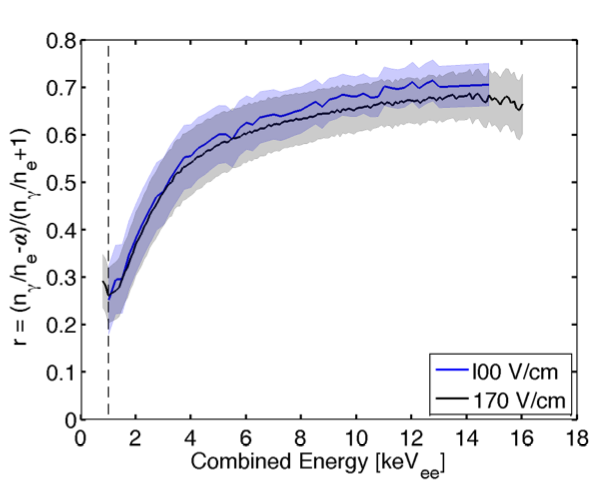
\includegraphics[width=120mm]{Chapter_Flucs/Figures/Iter1_100/R_comp.png}
\caption{Recombination Fraction at 170 V/cm (black) and 100 V/cm (blue). The shaded regions represent the one sigma of the observed fluctuations in recombination fractions $\rm \sigma_r$. The dashed line at 1.0 $\rm keV_{ee}$ represents the 50\% detection threshold.}
\label{fig:R_T}
\end{figure}


\subsection{Modeling the ER Band}

The main purpose of this section, and the tritium calibrations, are to be able to make predictions about WIMP sensitivity at various electric fields and in the WIMP search energies of interest, 1-5 $\rm keV_{ee}$. We now have the ability to reconstruct the electronic recoil band as it would appear with infinite detector resolution, with the ability to expand the band width by adding the measured detector resolution. Knowing the mean and width of the electronic recoil band and the mean of the NR band (described later) we can make predictions for ER and NR type discrimination which is a proxy for background event rejection.  

The mean of the ER band in discrimination space can be written as
\begin{equation}
\rm log_{10}(S2_b/S1) = log_{10} \left(\frac{(1-r)N_i}{(r+\alpha)N_i}\right) + log_{10}\left(\frac{g_2}{g_1}\right)
\label{eq:Band_Mean}
\end{equation}

\noindent where the observed charge and light signals $\rm S2_b$ and S1 have been converted to recombination probability r,  number of ions $\rm N_i$ and the exciton to ion ratio $\rm \alpha$ using equations \ref{eq:Gain} and \ref{eq:Quanta}.

The variance of the band can be written as,
\begin{equation}
\rm Var_{log_{10}(S2_b/S1)} = \frac{1}{\left(log(10)\right)^2} \times \sigma_R^2 \left( \frac{ - (\alpha+1) }{(1-r)(r+\alpha)N_i} \right)^2
\label{eq:Band_Var}
\end{equation}

\noindent Which has been written in terms of the number of ions $\rm N_i$, the recombination fraction r, and the measured recombination fluctuation $\rm \sigma_R$, defined to be $\rm \sigma_r\times N_i$. The result of the ER band's mean population and its corresponding 1 sigma fluctuation are shows in figure \ref{fig:ER_Band_Calc} for the case of 100 V/cm (blue) and 170 V/cm (black). This result shows the ER band with recombination fluctuations only. One can add light and charge collection fluctuations in quadrature to complete the modeling specific to any detector. Above 4 $\rm keV_{ee}$ the band separate as the higher drift field increased the charge extraction leading to better discrimination.

\begin{figure}[h!]\centering
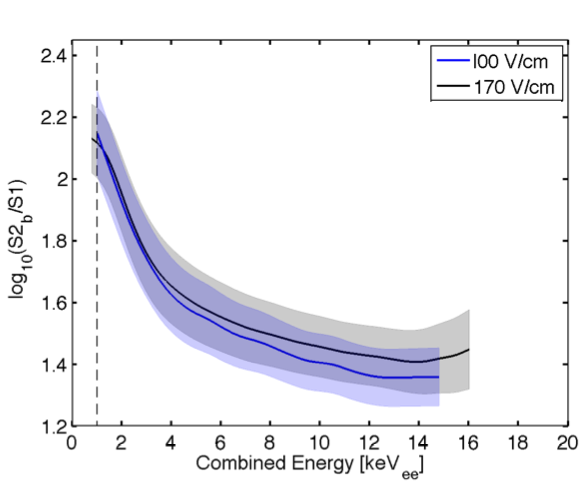
\includegraphics[width=130mm]{Chapter_Flucs/Figures/Iter1_100/Band_comp.png}
\caption{The result of the ER band's mean population and its corresponding 1 sigma fluctuation for the case of 100 V/cm (blue) and 170 V/cm (black). We find an over lap below 4 $\rm keV_{ee}$ where the additional strength of the drift field is hither improving threshold of discrimination. Above 4 $\rm keV_{ee}$ the band separate as the higher drift field increased the charge extraction leading to better discrimination.}
\label{fig:ER_Band_Calc}
\end{figure}

\newpage

\subsection{Measuring Alpha From the Tritium Data}

Having measured r and $\rm \sigma_r$ from the tritium calibration data the constancy of the exciton to ion ratio $\rm \alpha$ can be checked by requiring that as the number of ions tends to one the recombination fluctuations tend to that of a binomial process. This is justified as a single ion-electron pair will either recombine or not with some recombination probability r having a binomial variance written as,
\begin{equation}
\rm BinoVar= (1-r)rN_i
\label{eq:Bino_Var}
\end{equation}

\noindent where r is the recombination probability and $\rm N_i$ is the number of ions which can be thought of as the number of trials for the binomial process. In figure \ref{fig:Alpha_T} the y axis shows the ratio of the measured standard deviation of recombination to the standard deviation of a purely binomial process. The figure on the right has the expected binomial standard deviation on the x axis. The best alpha is one in which the observed standard deviation converges with that of a binomial process as the binomial variance tends to 1. The figure on the left has the number of ions available for recombination on the x axis. As the number of ions approaches one the standard deviation of recombination should become that of a binomial process. A single ion will either recombine or not with probability r.  The extrapolation is made by fitting the lowest energy bins above 90\% threshold 1.3 to 3 keV. Going below the value of one on the y axis implies that recombining electron-ion pairs have a variance better than binomial, which is unphysical if it is a random process.We find that the best intercept converging to a purely binomial process is with $\alpha$ = 0.20 consistent with the measurement in \cite{Doke_alpha} and not 0.06 as used in \cite{Dahl_Thesis}.

\renewcommand{\baselinestretch}{1}
\small\normalsize
\begin{figure}[h!]\centering
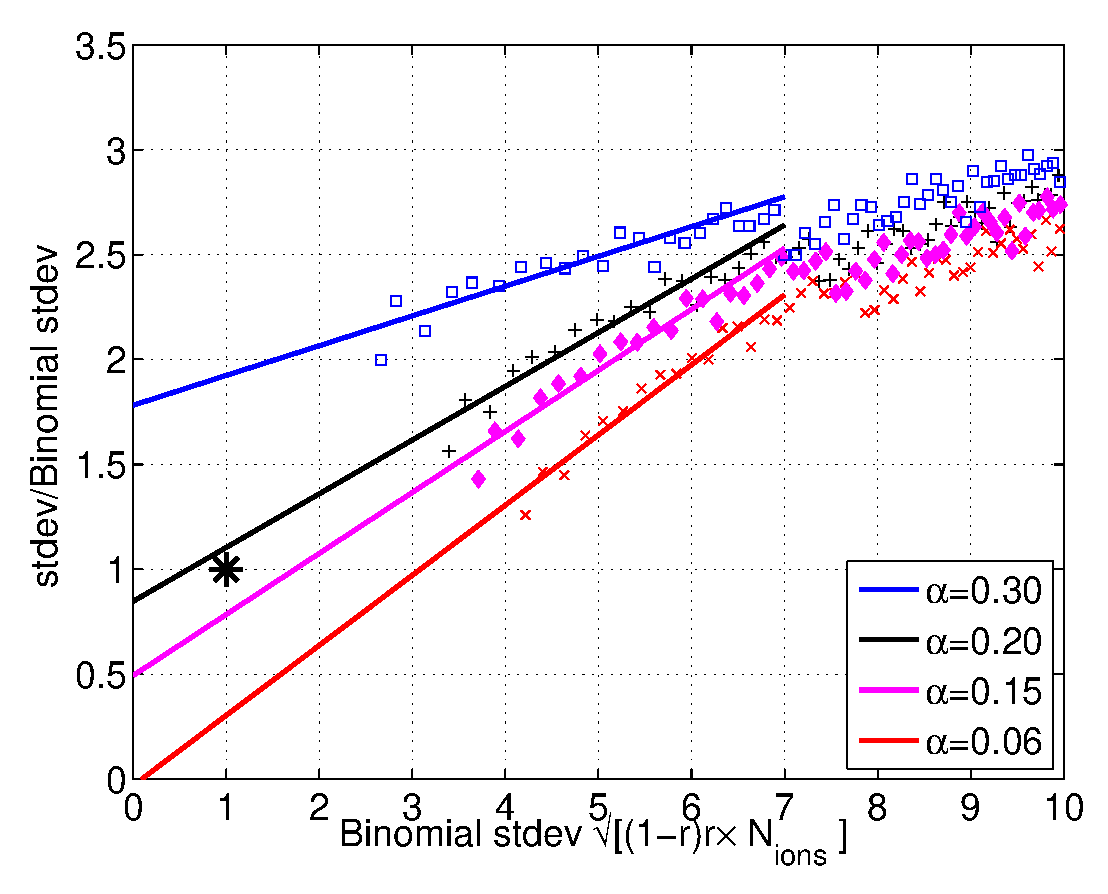
\includegraphics[width=74mm]{Chapter_Flucs/Figures/alpha/bino_norm_amp_iter1.eps}
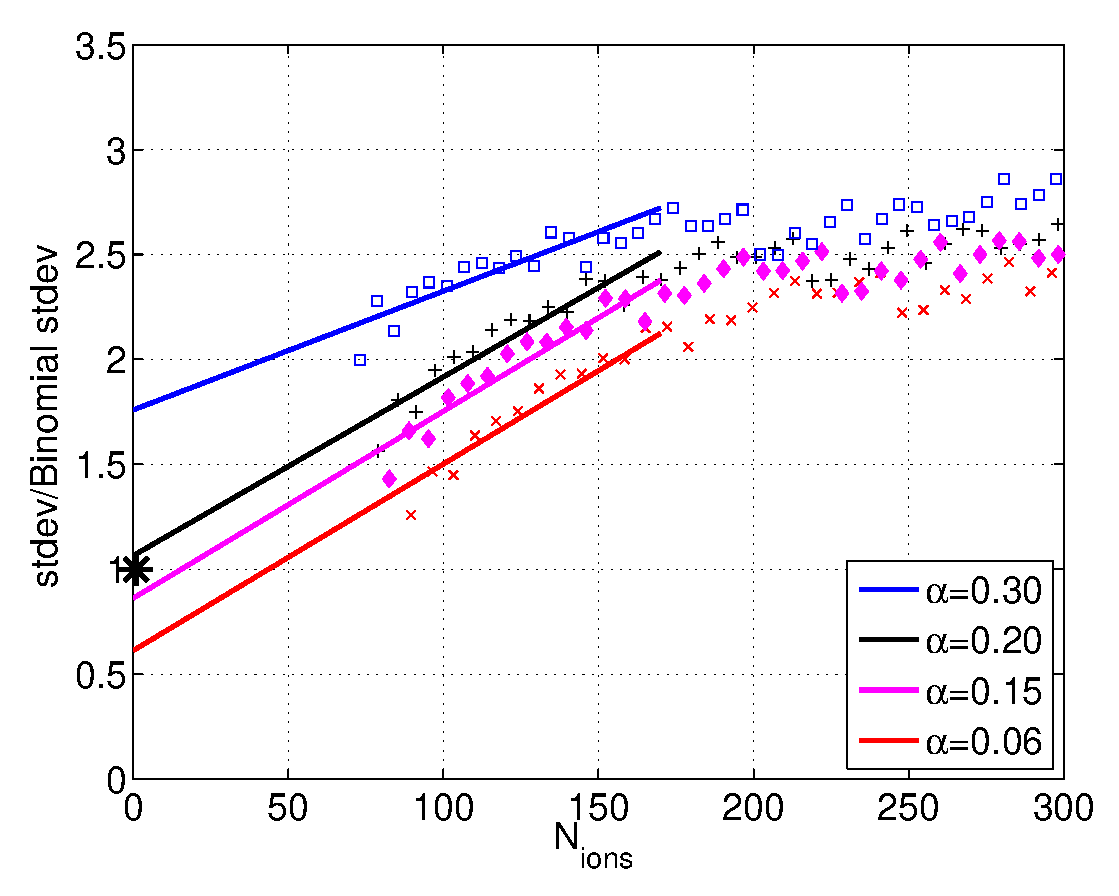
\includegraphics[width=74mm]{Chapter_Flucs/Figures/alpha/bino_norm_amp_ions_iter1.eps}
\caption{Determining the best $\rm \alpha$ using the tritium calibration data, with $\rm \alpha$ = 0.3(blue), 0.2(black), 0.15(magenta) and 0.06(red). Left: The y axis is the ratio of the measured standard deviation of recombination to that of a binomial processes and is plotted vs. the expected binomial standard deviation on the x axis. The best $\rm \alpha$ is one for which the observed standard deviation converges with that of a binomial process as the binomial variance tends to 1. Right, the same y axis as on the left but plotted vs. the number of ions available for recombination. As the number of ions approaches one the standard deviation of recombination should become that of a binomial process. A single ion will either recombine or not with probability r.  The best intercept converging to a purely binomial process (black star) is with $\rm \alpha$ = 0.20. Falling below the value of one on the y axis implies that recombining electron-ion pairs have a variance better than binomial, which is unphysical if it is a random process. Note, the fits use only data above 90\% threshold at 1.3 keV, starting from the third data point from the left. The higher end cut off at  3 keV corresponds to the end of the fitted lines. }
\label{fig:Alpha_T}
\end{figure}
\renewcommand{\baselinestretch}{2}
\small\normalsize

\newpage

\section{Extracting Recombination Fluctuations from $\rm ^{137}Cs$ Calibration}

To expand the picture of recombination fluctuation to higher energies the same method used for the tritium calibration was applied to the Compton edge of a $\rm ^{137}Cs$ external calibration source. The $\rm ^{137}Cs$ source provides ER calibration data from the backscatter peak around 150 keV to the photo peak at 662 keV. Figure \ref{fig:Cs_LYQYR} on the left shows the measured mean number of photons, electron in each energy bin along with their one sigma fluctuation (shaded). The number of excitons and ions are also show assuming an $\alpha$ = 0.20. Once the mean number of photons and electrons are measured the recombination probability is determined and plotted on the right in figure \ref{fig:Cs_LYQYR}. The inflection around 662 keV is due to the sharp rise and fall of the photo peak skewing the measurement of number of photons and electrons.

\begin{figure}[h!]\centering
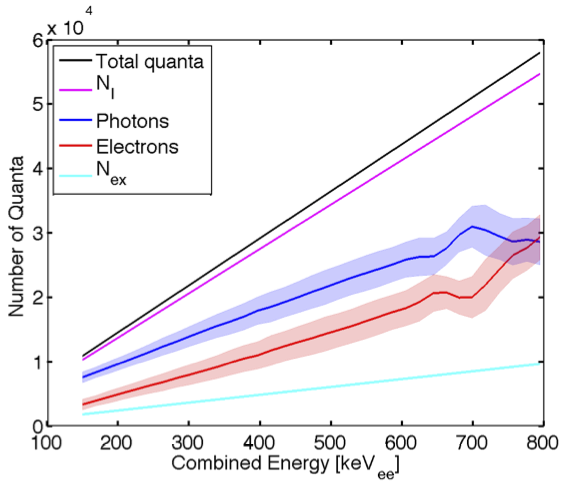
\includegraphics[width=72mm]{Chapter_Flucs/Figures/Cs/quanta_cs_.png}
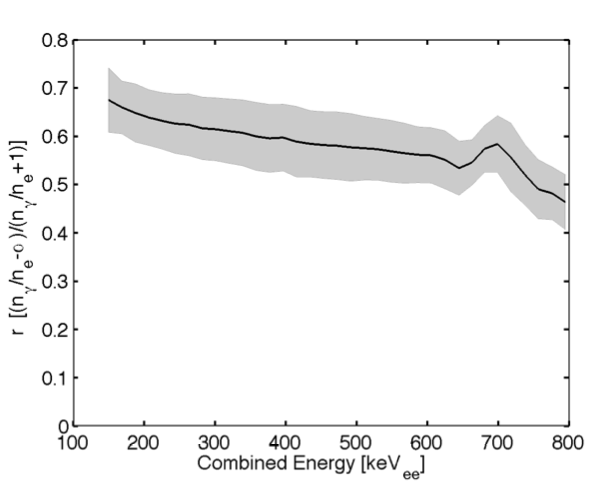
\includegraphics[width=72mm]{Chapter_Flucs/Figures/Cs/R_cs_.png}
\caption{ Left: The mean and one sigma standard deviation of the measured number of photons (blue) and electrons (red). Also shown is the total quanta (in black) which is the sum of photons and electrons and the expected number of ions (magenta) and excitons (cyan) using $\rm \alpha$ = 0.20. Right: The recombination probability r (solid black) and the one sigma fluctuation $\rm \sigma_{r}$ (shaded). }
\label{fig:Cs_LYQYR}
\end{figure}

\newpage

\section{Recombination Fluctuations, The Bigger Picture}
We have now measured the recombination probability and fluctuation over a wide range of energies and at two fields for tritium (100 and 170 V/cm). The calibrations range from the 1.0 keV 50\% threshold with tritium to about 700 keV with the $\rm^{137}Cs$ calibration, and include the line sources used for the energy calibration in \ref{Ch:E_Scale_Cal} and table \ref{table:Cal_lines}. Also shown is a $\rm ^{57}Co$ calibration at a variety of electric fields ranging from 60 to 5000 V/cm from \cite{Dahl_Thesis}. Figure \ref{fig:R_Big} on the left shows the observed recombination fluctuation $\rm \sigma_R$ measurements vs. the standard deviation expected from a purely binomial process (equation \ref{eq:Bino_Var}). At our field of 100 and 170 V/cm we find good agreement with a simple power law fit which can be thought of as the fluctuation receiving an amplification over the underlying binomial process.

 Figure \ref{fig:R_Big} on the right shows the measured recombination fluctuation $\rm \sigma_R$ vs. the number of ions available for recombination $\rm N_i$. The x axis is chosen to be number of ions as recombination fluctuations only act on ions and not excitons, the conversion to energy on the x axis is simply $\rm E = W\times n_i (1 + \alpha ) $. It is found that the measured recombination fluctuation can be well described by a generic power law fit.

\renewcommand{\baselinestretch}{1}
\small\normalsize
\begin{figure}[h!]\centering
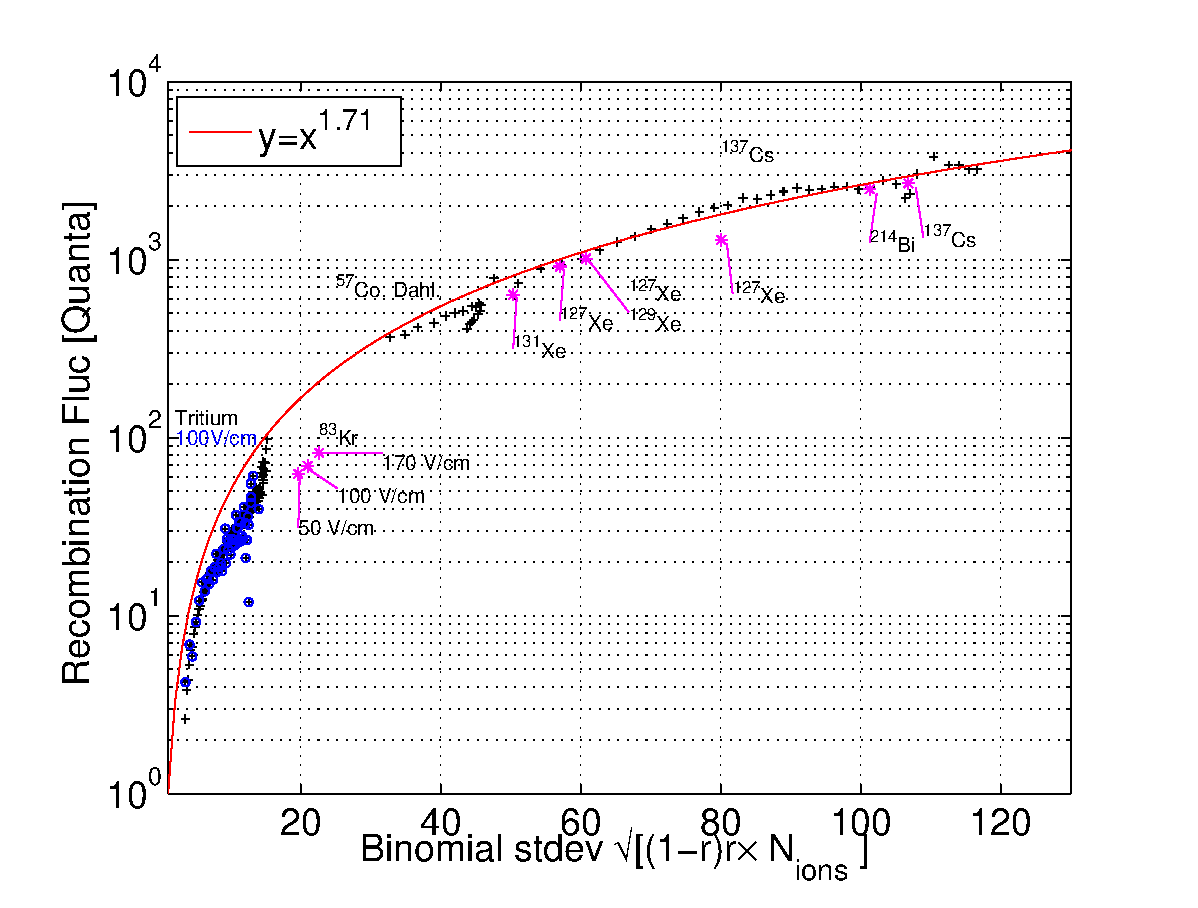
\includegraphics[width=73mm]{Chapter_Flucs/Figures/alpha/bino_amp_100_iter1.eps}
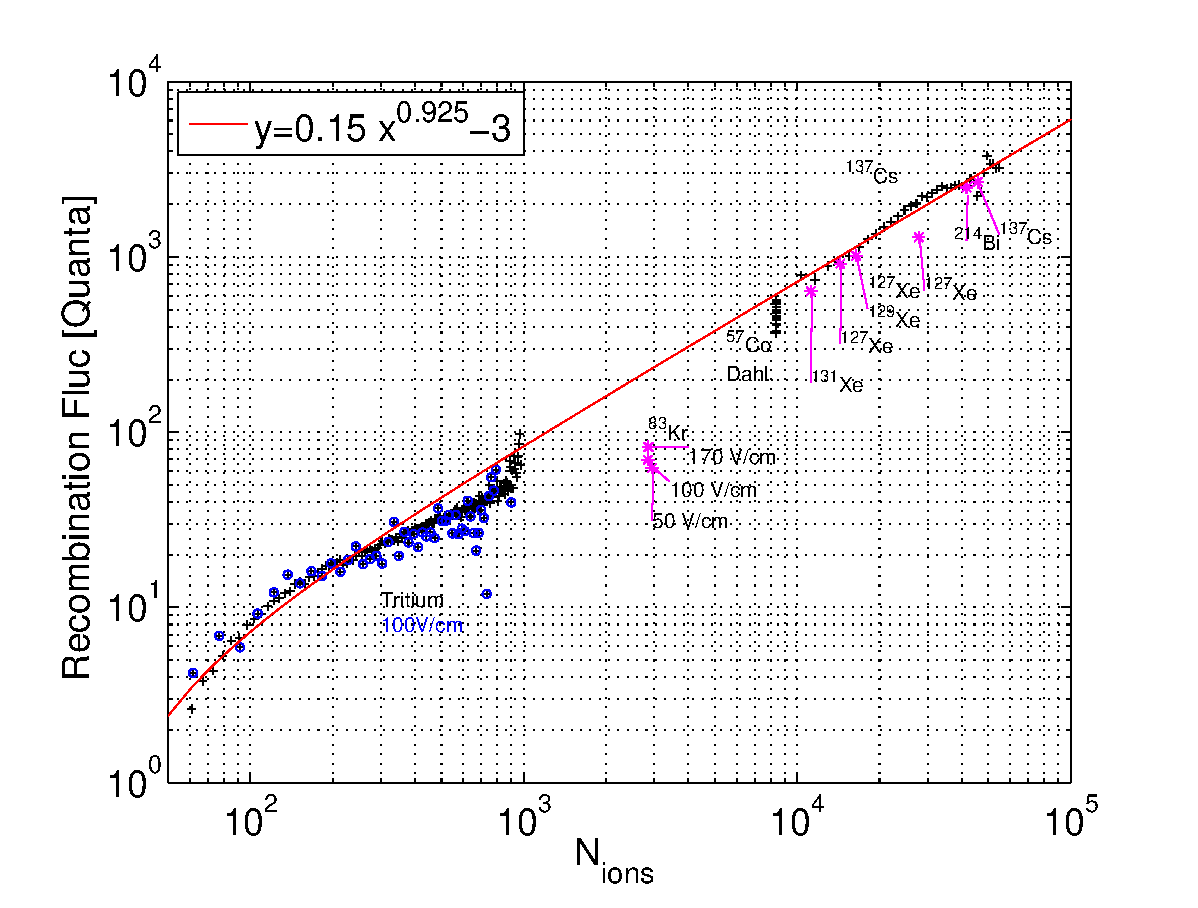
\includegraphics[width=73mm]{Chapter_Flucs/Figures/alpha/R_v_Ni_100_iter1.eps}
\caption{ Recombination fluctuations measurements are labeled on the plot and include data from tritium at 170 V/cm, tritium at 100 V/cm, $\rm ^{137}Cs$ calibration, the line sources used for the energy scale calibration listed in table \ref{table:Cal_lines} and a $\rm ^{57}Co$ calibration at a variety of electric fields ranging from 60 to 5000 V/cm from \cite{Dahl_Thesis}. Left: the observed recombination fluctuation $\rm \sigma_R$ measurements vs. the standard deviation expected from a purely binomial process,equation \ref{eq:Bino_Var}. The red curves represent power law fits to the data.}
\label{fig:R_Big}
\end{figure}
\renewcommand{\baselinestretch}{2}
\small\normalsize

There is no physical justification for the power law fit in figure \ref{fig:R_Big} to the apparent binomial variance amplification. This is a fatal flaw in our recombination model. The observed variance is off by roughly a factor of $\rm N_{ions}$, surpassing 1000 in the cesium data. The recombination model we are using assumes that every electron ions pair is a separate entity that either recombines or not, thus the variance should be binomial. There is another issue with the recombination model. The decline of recombination probability as the energy (or $\rm N_i$) tends to zero is unphysical yet is observed in the data, shown in figure \ref{fig:R_T}. The probability of the electron ion-pair to recombine should be insensitive to the number of electron-ion pairs created by the energy deposit. We take this as a first clue to solving the problem and outline the consequences of allowing for electron-ion pair mixing with some encounter probability in the next two sub-sections. Culminating with a model which will simultaneously reproduce the observed recombination fraction, explain its decline at low energy, and yield the correct recombination fluctuations.

\newpage 

\subsection{Encounter Recombination Probability}

The apparent amplification of the observed ER fluctuations over that of a binomial process is troubling. What causes the ER events to be so erratic over their nuclear recoil counterparts which can be well described by binomial fluctuation \cite{Dahl_Thesis}. The key difference that lends a clue to solving the puzzle is that for a given energy nuclear recoils will produce significantly less election-ion pairs. It has been observed for ER events that as the number of ions goes to one the recombination fluctuations do indeed become more binomial like, shown in figure \ref{fig:Alpha_T}. Before we move on, it should be noted that the method outlined in this section will succeed in explaining recombination fluctuation but will fail to reproduce the recombination fraction probability. This subsection is meant as a discussion on encounter recombination probability leading to the model in the subsection to follow that will bridge measuring recombination probability and its variance.

In order to tackle the issue of recombination fluctuations we introduce encounter recombination probably $\rm r_\epsilon$. The term $\rm r_\epsilon$ will couple freed electrons to ions other than its own. There are well motivated arguments to be made to include a $\rm r_\epsilon$ term. First, in liquid xenon the decay of the calibration source \KrCal has been observed to receive an enhancement of several percent in the light yield of the second 9.4 keV following the first decay of 32.1 keV \cite{Start_Kr}. This can be attributed to the second decay occurring surrounded by a ball of charge from the first decay resulting in an enhanced encounter recombination probability and increased light yield. The two \KrCal decays are separated by a half life to 154 ns \cite{83Kr_HalfLife_1}. The shorter the timing separation between the two decays the greater the light yield enhancement, with light yield enhancement observed past 1000 ns \cite{Kastens}, \cite{Baudis} [LUX data shows enhancement out to 2000 ns could add this plot to thesis...]. This lends evidence that freed electrons can be attracted to ions while diffusing from the interaction site on the time scales of hundreds of nano seconds. Further, the idea of encounter probability was worked out by Mozumder noting the need for encounter recombination probabilities of 0.01 in order to explain the ion production rate in liquid xenon \cite{Mozumder}. 

In this subsection we set out to model the variations resulting from the recombination porbability containing a component from encounter recombination probability. Once the model for variance is worked out we can fit to the tritium and $\rm^{137}Cs$ calibration data in order to extract the encounter recombination probability. 

First we start with expression for the variance of a binomial process with some recombination probability r. 

\begin{equation}
\rm Var_r= (1-r)rN_i
\label{eq:Bino_Var2}
\end{equation}

\noindent where $\rm N_i$ is the number of ions, and can be thought of as the number of trials. Next we split the total observed recombination probability into two components.

\begin{equation}
\rm r=r_s + r_\epsilon
\label{eq:rs}
\end{equation}

\noindent where $\rm r_s$ is the self recombination probability and $\rm r_\epsilon$ is the encounter recombination probability. The expectation is that  $\rm r_\epsilon << r_s$, \cite{Mozumder}. The variance resulting from the two terms can be considered as independent processes occurring subsequently thus, the total variance of the process is the the sum of the individual variances for each ion. In our modeling every free electron has an average encounter probability $\rm r_\epsilon$ with each ion. The variance of $\rm N_i$ ions is given in equation \ref{eq:Bino_Var2} and is illustrated in figure \ref{fig:Flucs_Fig} for the case of one ion. At this point we pause to point out the fatal fall in this theory. As the number of ion-electron pairs grow all ions will recombine as each ion is unable to avoid recombination from the bombardment of $\rm N_i$ electrons. The observed recombination probability for this process becomes $\rm r=r_s + N_i\cdot r_\epsilon$. With that note, we proceed to learn more about encounter recombination probability. 

\renewcommand{\baselinestretch}{1}
\small\normalsize
\begin{figure}[h!]\centering
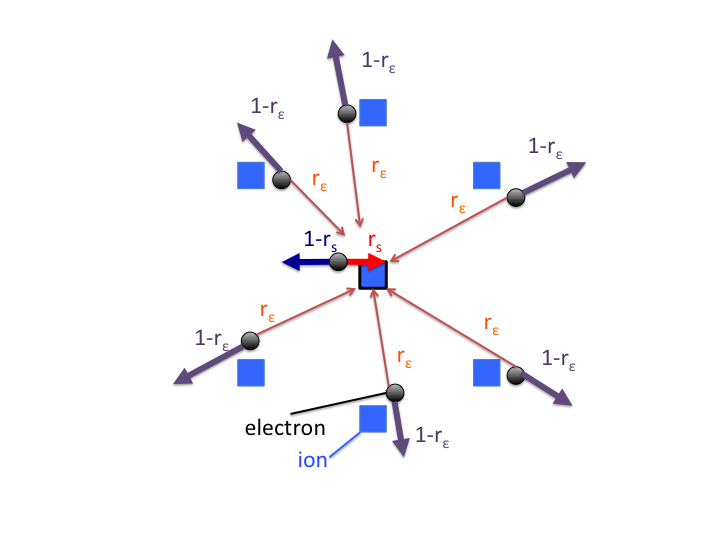
\includegraphics[width=150mm]{Chapter_Flucs/Figures/Recomb_Flucs/Bino_Var_ER.png}
\caption{Illustration of recombination for the case of a in single ion, blue box highlighted in black at the center. The total recombination probability for one ion is the combination of the the dominant self recombination probability ($\rm r_s$) plus the sum of the encounter recombination probabilities ($\rm r_\epsilon$) from the remaining N-1 electrons. This process is repeated for N number of ion electron pairs leading to a binomial variance given in equation \ref{eq:Var_s}. }
\label{fig:Flucs_Fig}
\end{figure}
\renewcommand{\baselinestretch}{2}
\small\normalsize


\begin{equation}
\rm Var_{(r_s + r_\epsilon)} = \sum\limits_{N_i}r_s(1-r_s) + \sum\limits_{N_i} r_\epsilon(1-r_\epsilon)(N_i-1)
\label{eq:Var_s}
\end{equation}

\noindent the first term of equation \ref{eq:Var_s} is the binomial variance of a single electron-ion pair with some probability $\rm r_s$ to recombine. The second term is the binomial variance of the average encounter probability $\rm r_\epsilon$ with all other electrons excluding its own escaped electron, a total of ($\rm N_i$-1). Both terms are summed over all possible ions, accounting for all $\rm N_i$ ions with $\rm N_i -1$ electrons available to be encountered. Due to the relatively slow mobility of ions vs electrons, the ions are treated as fixed with the freed electrons having some probability of encounter an ion. This is a simplistic model that treats the encounter probability as an overall average for all electron-ion pair combinations. Assuming $\rm N_i$ is large equation \ref{eq:Var_s} can be simplified to 

\begin{equation}
\rm Var_{(r_s + r_\epsilon)} = r_s(1-r_s)N_i + r_\epsilon(1-r_\epsilon)N_i^2
\label{eq:Var_s2}
\end{equation}

The result of splitting the recombination probability into self and encounter recombination is subtle, yet has huge implications. Comparing equation \ref{eq:Bino_Var2} to \ref{eq:Var_s} we find that the binomial variance of the process with encounter recombination probability will grow like $\rm N_i^2$ as opposed to the binomial variance of a self recombination process that grows like $\rm N_i$. To better understand the amplification of the binomial fluctuation observed in the data, figure \ref{fig:R_Big}, we define an amplification term as the ratio of the binomial variance with encounter recombination probability to that of a binomial process with self recombination probability r.

\begin{equation}
\rm \mathcal{A}= \frac{Var_{(r_s + r_\epsilon)}}{Var_r}
\label{eq:Amp}
\end{equation}

\noindent $\rm Var_{(r_s + r_\epsilon)}$ and $\rm Var_r$ are given in equations \ref{eq:Var_s2} and \ref{eq:Bino_Var2}, respectively. 


We will treat two cases. First, we will assume that $\rm r_\epsilon << r_s$ and $\rm r_s \simeq r$. Second, we will hold the ratio of $\rm r_\epsilon/r$ to be a constant. The second case is motivated by the idea that electric field and energy dependance that governs self recombination probability also applies to encounter recombination probability.

The amplification of the binomial variance from equation \ref{eq:Amp} is

\begin{equation}
\rm \mathcal{A} =\frac{N_i}{N_i} \left( \frac{ r_s(1-r_s) + r_\epsilon(1-r_\epsilon)N_i }{ r(1-r) } \right)
\label{eq:Amp_S1}
\end{equation}

\noindent assuming that $\rm r_\epsilon << r_s$ and $\rm r_s \simeq r$ equation \ref{eq:Amp_S1} can be simplified to, 

\begin{equation}
\rm \mathcal{A} =\left(1 +  \frac{ r_\epsilon(1-r_\epsilon)N_i }{ r(1-r) } \right)
\label{eq:Amp_S2}
\end{equation}
 
\noindent  Using equation \ref{eq:Amp_S2} the value of encounter recombination probability $\rm r_\epsilon$ can be extracted from the tritium and $\rm^{137}Cs$ data using $\rm N_i$, r, and $\rm \mathcal{A}$.  Where the value of binomial amplification $\rm \mathcal{A}$ is the extracted from the data defined as the recombination fluctuation $\rm \sigma_R$ over $\rm \sigma_R$-binomial, shown in figure \ref{fig:R_Big}. The result of extracting encounter recombination probability $\rm r_\epsilon$ is shown in figure \ref{fig:Encounter_R_Const}. The overall average of  $\rm r_\epsilon$ from the calibration data is $\rm r_\epsilon$ = 0.0042 varying from 0.002 to 0.007, in good agreement with Mozumder \cite{Mozumder}.

\renewcommand{\baselinestretch}{1}
\small\normalsize
\begin{figure}[h!]\centering
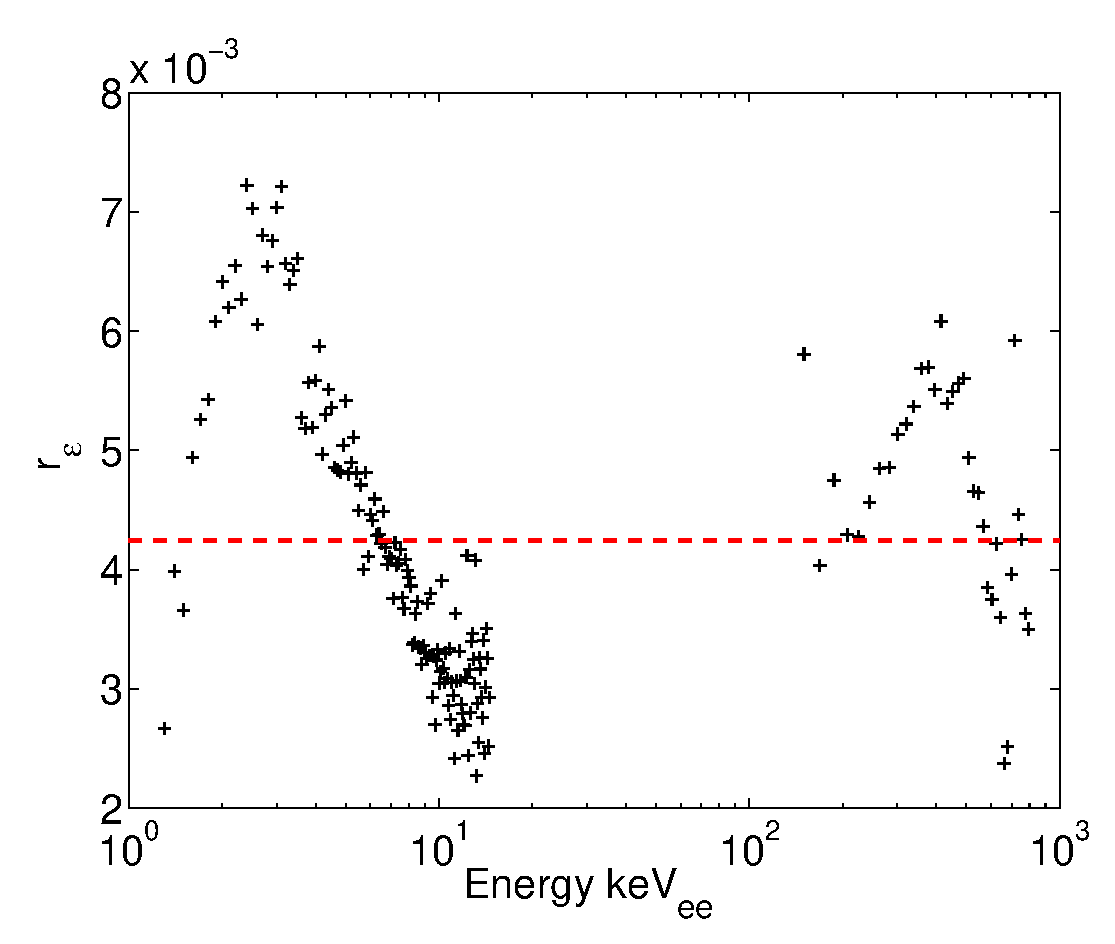
\includegraphics[width=73mm]{Chapter_Flucs/Figures/Recomb_Flucs/E_const.eps}
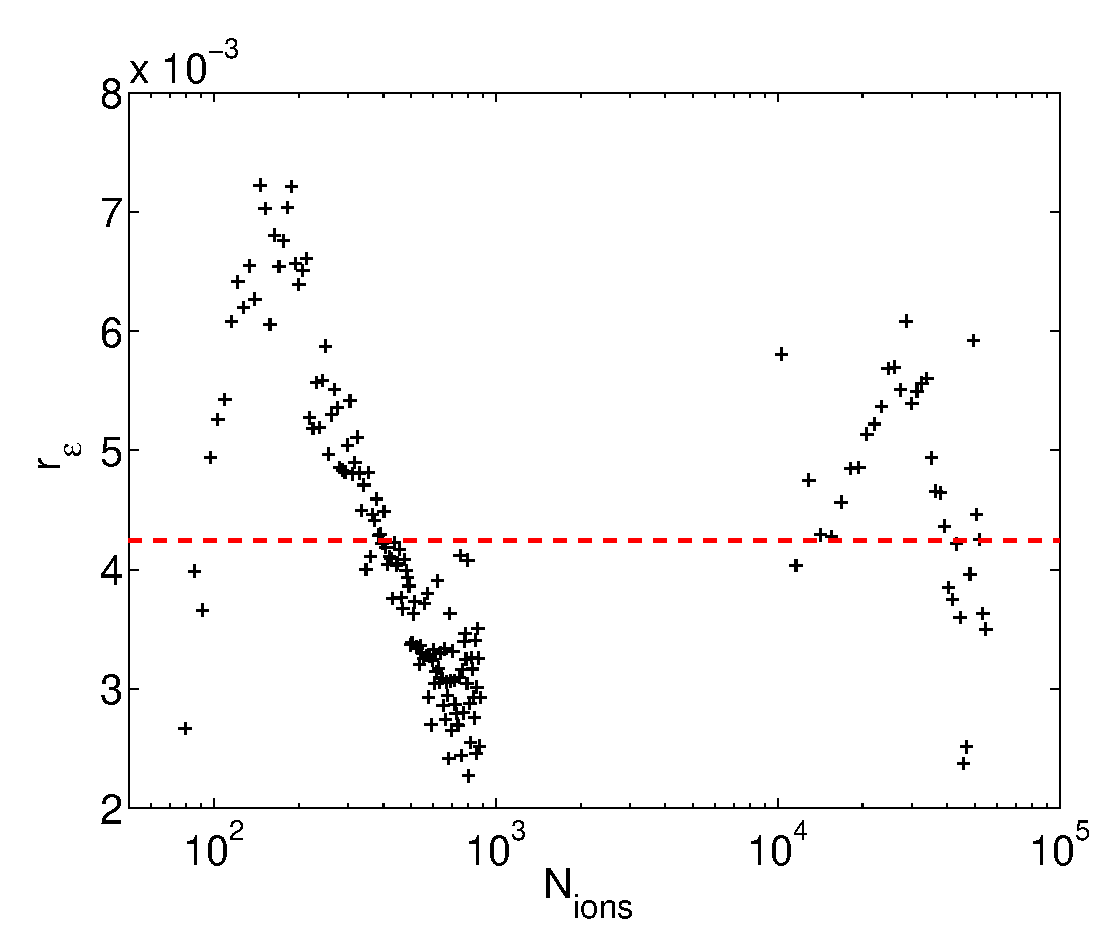
\includegraphics[width=73mm]{Chapter_Flucs/Figures/Recomb_Flucs/Ni_const.eps}
\caption{ Encounter recombination probability $\rm r_\epsilon$ extracted from the tritium and $\rm^{137}Cs$ calibration data at 170 V/cm, derived from equation \ref{eq:Amp_S2}. Left plotted vs. energy in keV. Right: plotted vs. the number of ions. The solid red line represents the overall average of $\rm r_\epsilon$ from the calibration data is $\rm r_\epsilon$ = 0.0042. }
\label{fig:Encounter_R_Const}
\end{figure}
\renewcommand{\baselinestretch}{2}
\small\normalsize

\newpage

Taking the value of $\rm r_\epsilon$ as a constant of 0.0042 we find that the observed ER recombination fluctuations are infact consistent with binomial fluctuation at our field of 170 and 100 V/cm, shown later in figure \ref{fig:Flucs_Model}. This is a step in the right direction for understanding recombination fluctuations. Our data is limited to only two electric fields at 100 and 170 V/cm making it difficult to model field dependance. To expand the model we include data from Dahl, using a $\rm ^{57}Co$ source with fields ranging from 60 to 5000 V/cm \cite{Dahl_Thesis}. We then extract $\rm r_\epsilon$, shown as the black points in figure \ref{fig:Encounter_R_All}.

\renewcommand{\baselinestretch}{1}
\small\normalsize
\begin{figure}[h!]\centering
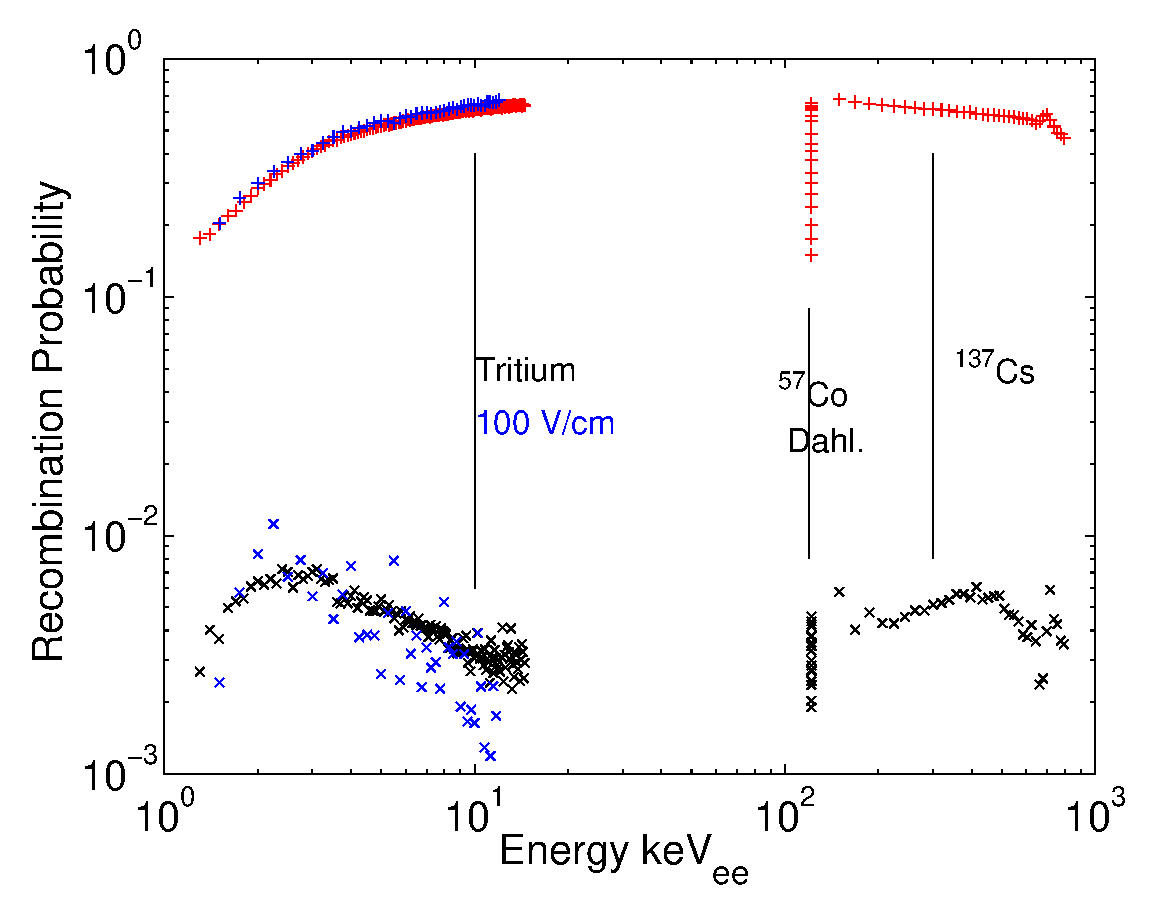
\includegraphics[width=120mm]{Chapter_Flucs/Figures/Recomb_Flucs/E_r_re.eps}
\caption{ The red crosses indicate the total recombination probability r for the calibration sources labeled on the plot. The black x-s indicate the encounter recombination probability $\rm r_\epsilon$. The blue points indicate the tritium data at 100 V/cm. The data includes tritium at 170 V/cm (black), tritium at 100 V/cm (blue), $\rm ^{137}Cs$ and data from Dahl for $\rm^{57}Co$ ranging from 60 to 5000 V/cm \cite{Dahl_Thesis}.}
\label{fig:Encounter_R_All}
\end{figure}
\renewcommand{\baselinestretch}{2}
\small\normalsize

The data from Dahl, shown in \ref{fig:Encounter_R_All}, provides good motivation to proceed with our second assumption, modeling the ratio of $\rm r_\epsilon/r$ to be a constant. There appears to be correlation between the recombination probability and the encounter recombination probability. This correlation is sensible, considering that as the electric field is increased the freed electrons can escape the ions more readily. Thus, both the self and encounter recombination decline as a function of applied electron field. However, the assumption that $\rm r_\epsilon$ and r are always correlated is to be taken with a grain of salt, and is not supported by the tritium data. Between 2.5 and 10 keV the recombination probability r and $\rm r_\epsilon$ become anti-correlated. With that caveat mentioned, we proceed with the second case.

\begin{equation}
\rm r_\epsilon = r_{\epsilon_0} + \mathcal{C} r
\label{eq:Case_2}
\end{equation}

\noindent where $\rm \mathcal{C}$ is a constant linking the observed recombination probability r to $\rm r_\epsilon$. The best fit for both cases is show in figure \ref{fig:Flucs_Model}. Case one, is with a global average of $\rm r_\epsilon$= 0.0042, extracted from the tritium and $\rm^{137}Cs$ data. Case two, is using $\rm r_\epsilon$ = 0.0011 + 0.006r. The fit for case one is within 30\% when excluding the data from Dahl, and the fit the second case deviates less than 30\% from all of the data.

\renewcommand{\baselinestretch}{1}
\small\normalsize
\begin{figure}[h!]\centering
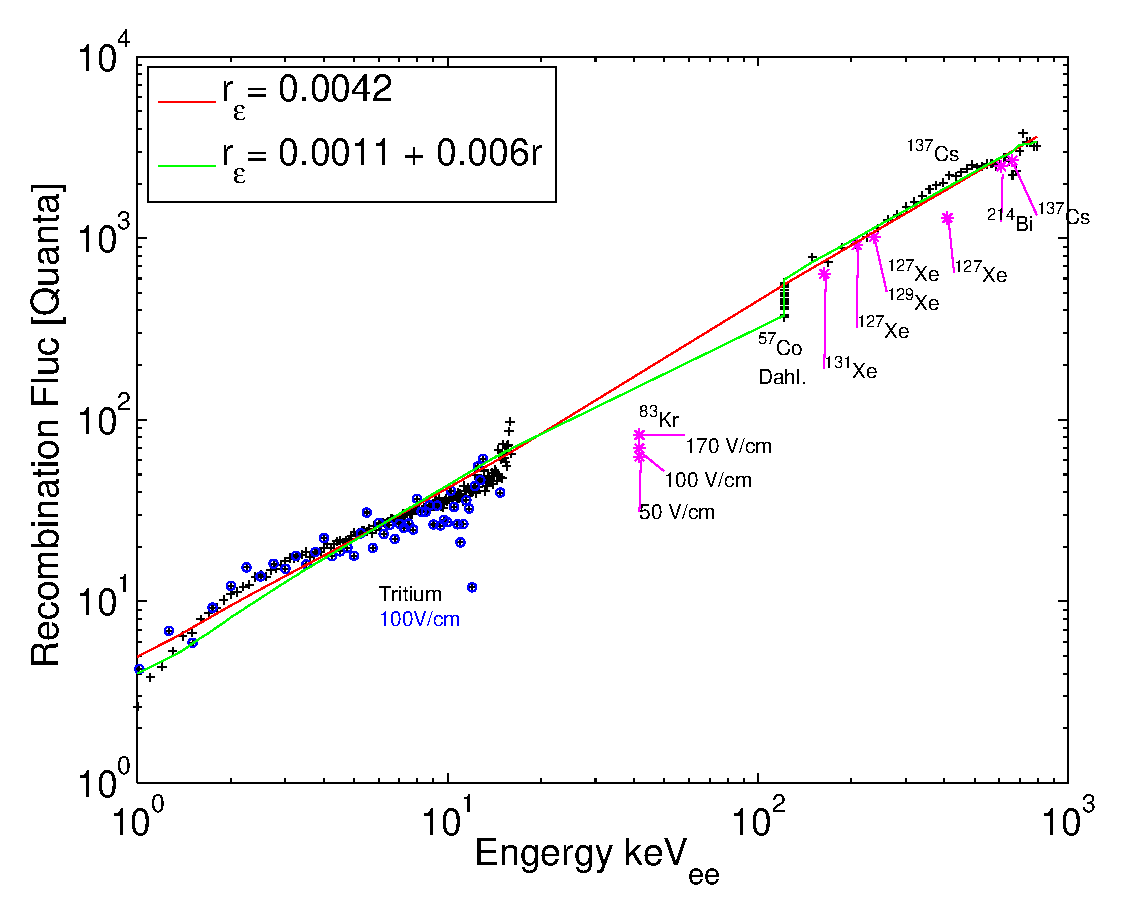
\includegraphics[width=120mm]{Chapter_Flucs/Figures/Recomb_Flucs/R_v_E_model_iter1.eps}
\caption{ Fit to the observed ER recombinations modeled with binomial fluctuations where the recombination probability includes a encounter recombination component. Case one (red) is with a assuming a constant $\rm r_\epsilon$= 0.0042, extracted from the tritium and $\rm^{137}Cs$ data. Case two (green) is using $\rm r_\epsilon$ = 0.0011 + 0.006r. Case two is in significantly better agreement with the field dependent data from Dahl, as it accounts for field effects \cite{Dahl_Thesis}. The fit for case two (green) deviates less than 30\% from the data.}
\label{fig:Flucs_Model}
\end{figure}
\renewcommand{\baselinestretch}{2}
\small\normalsize

The simplistic model outlined in this subsection demonstrates that recombination fluctuation of electronic recoil can indeed be the result of binomial statistics. Remarkably, a sub 1\% component of recombination probability r from encounter probability leads to an apparent binomial amplification factor of 1 to 1000, shown in the right plot in figure \ref{fig:R_Big}. The tiny value of $\rm r_\epsilon$ makes a significant impact when considering the combinatorics of the recombination process. This is good progress, we have found a simplistic was to gain an additional factor of $\rm N_i$ for recombination fluctuations vs. energy, instead of applying a power law fit to binomial amplification with no physical basis. However, we still need to clean up the problem of total ion-electron pair recombination resulting from such a model. We have found the correct variance but have failed to produced the correct recombination probability. The fix the the issue is described in the next subsection.


\subsection{Clusters of Encounter Recombination}

In the previous subsection a model was introduced which could predict the observed recombination fluctuations of ER events. However, the model failed to produce the correct recombination probability. We found that as the energy (or $\rm N_i$) rises the recombination probability tends to 1, and beyond as $\rm r=r_s + N_i\cdot r_\epsilon$. The zeroth order correction to this problem is to remove the self recombination term $\rm r_s$ and treat self recombination as just another encounter recombination probability, $\rm r_s=r_\epsilon$. Next, we will not allow the full $\rm N_i$ electrons to interact with each ion as this is unphysical. Instead, only a small number of the total ions $\rm N_\epsilon$ are allowed to have encounters for each energy deposit, illustrated in \ref{fig:Flucs_Fig}. The value of $\rm N_\epsilon$ is set by the requirement to reproduce the correct recombination probability. The observed recombination probability r is then written as,

\begin{equation}
\rm r=r_s+(N_\epsilon-1) r_\epsilon = N_\epsilon r_\epsilon
\label{eq:Simp1}
\end{equation}

\noindent where r is the observed recombination probability at a given energy, $\rm r_s$ is the self recombination probability taken to be equal to the encounter recombination probability $\rm r_\epsilon$, and $\rm N_\epsilon$ is the average number of electron encounters for each ion. Note that the value of $\rm N_\epsilon$ used is an average and can also vary event to event depending on the ER track geometry. The equation for recombination probability in \ref{eq:Simp1} inadvertently solves the other issue of the original recombination model. By taking self recombination $\rm r_s$ to be equal to $\rm r_\epsilon$ the observed recombination probability r naturally vanishes as the energy ($\rm N_i$) tends to zero, as observed in the data shown in figure \ref{fig:R_T}. The binomial variance of such a process is,

\begin{equation}
\rm Var_{N_\epsilon r_\epsilon} = (1-N_\epsilon r_\epsilon)N_\epsilon r_\epsilon N_i
\label{eq:SimpVar}
\end{equation}

\noindent where $\rm Var_{N_\epsilon r_\epsilon} $ is the recombination variance in number of quanta squared for a given interaction with $\rm N_i$ ions, encounter recombination probability $\rm r_\epsilon$ with an average of $\rm N_\epsilon$ encounters. The variance derived in equation \ref{eq:SimpVar} grown like $\rm N_i$ and suffers the same problem as our original model. The variance needs to grow like $\rm N_i^2$ to explain the observed recombination fluctuations in the data, as seen in the previous subsection. 

The solution is surprisingly straight forward considering the two requirements. First, in order to maintain the correct recombination probability r the value of  encounter interactions $\rm N_\epsilon$ must be fixed. Second, to get the additional factor of $\rm N_i$ in variance the process of size  $\rm N_\epsilon$ must be be repeated, with the repetition scaling like $\rm N_i$. Remember, we are only allowing a small number, $\rm N_\epsilon$, of the total ions available ions to have encounters. Consider the picture in figure \ref{fig:Flucs_Fig} but for $\rm N_\epsilon$ encounters repeated $\rm N_i/N_\epsilon$ times in $\rm N_C$ clusters, such a process is illustrated in figure \ref{fig:Flucs_Fig_Cluster}. The number of clusters $\rm N_C$ for a given in equation \ref{eq:N_C}. 

\begin{equation}
\rm N_C = N_i/N_\epsilon
\label{eq:N_C}
\end{equation}


\renewcommand{\baselinestretch}{1}
\small\normalsize
\begin{figure}[h!]\centering
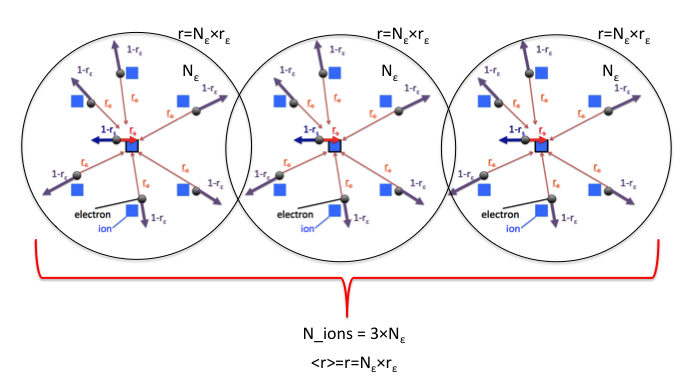
\includegraphics[width=150mm]{Chapter_Flucs/Figures/Recomb_Flucs/Bino_V_Cluster.png}
\caption{Illustration of recombination for the case of a in single ion occurring in $\rm N_C$ clusters with number of encounters $\rm N_\epsilon$. The total recombination probability for all clusters is equal to the average of each individual cluster. In each cluster the recombination probability is equal to the number of interaction $\rm N_\epsilon$ times the encounter recombination probability $\rm r_\epsilon$. The process is repeated for $\rm N_C$ clusters, resulting in and additional factor $\rm N_i$ in the observed variance while maintaining the correct average recombination probability r. }
\label{fig:Flucs_Fig_Cluster}
\end{figure}
\renewcommand{\baselinestretch}{2}
\small\normalsize

The value $\rm N_\epsilon$ can be considered as the number of encounters per cluster, or generalized to the number of ions per cluster. The electron-ion pairs have $\rm N_\epsilon$ encounters in each cluster with an average recombination probability r. The total recombination probability of the system of clusters remains equal to $\rm r=\rm N_\epsilon r_\epsilon$ without blowing up to unity. Since the process is repeated for $\rm N_C$ clusters the variance from equation \ref{eq:SimpVar} becomes

\begin{equation}
\rm Var_{N_\epsilon r_\epsilon} =  \sum\limits_{N_C}(1-N_\epsilon r_\epsilon)N_\epsilon r_\epsilon N_i
\label{eq:SimpVar_C}
\end{equation}

\noindent where $\rm Var_{N_\epsilon r_\epsilon} $ is the recombination variance of equation \ref{eq:SimpVar} for $\rm N_C$ clusters. Plugging in the value of $\rm N_C$ from equation \ref{eq:N_C} we find

\begin{equation}
\rm Var_{N_\epsilon r_\epsilon} =  (1-N_\epsilon r_\epsilon)N_\epsilon r_\epsilon N_i (N_i/N_\epsilon)
\label{eq:SimpVar_C}
\end{equation}

\noindent where the multiplication by $\rm N_C$ is written as $\rm N_i/N_\epsilon$. Further simplifying equation \ref{eq:SimpVar_C} and recalling that $\rm r=N_\epsilon r_\epsilon$,

\begin{equation}
\begin{split}
\rm Var_{N_\epsilon r_\epsilon} =  (1-N_\epsilon r_\epsilon) r_\epsilon N_i^2 \\
\rm Var_{N_\epsilon r_\epsilon} =  (1-r) r_\epsilon N_i^2 \\
\rm Var_{N_\epsilon r_\epsilon} =  (1-r) r \frac{N_i^2}{N_\epsilon} 
\end{split}
\label{eq:SimpVar_C_2}
\end{equation}

\noindent Taking the result for variance given in equation \ref{eq:SimpVar_C_2} we calculate the apparent amplification factor $\rm \mathcal{A}$ over that of a binomial process, our original recombination theory. 

\begin{equation}
\begin{split}
\rm \mathcal{A} = \frac{Var_{N_\epsilon r_\epsilon}}{Var_{r}} = \frac{(1-r)r N_i^2/N\epsilon}{(1-r)rN_i} \\
%\rm \mathcal{A} = \frac{r_\epsilon N_i}{r} \\
\rm \mathcal{A} = \frac{N_i}{N_\epsilon} = N_C
\end{split}
\label{eq:Simp_Amp}
\end{equation}

\noindent the amplification factor in equation \ref{eq:Simp_Amp} remarkably simple. The amplification over that of a binomial process reduces to the number of clusters $\rm N_C$. Note, the value of $\rm N_\epsilon$ is the ratio of $\rm r/r_\epsilon$. This is the key to the cluster recombination model. We have picked up an additional factor $\rm N_i$ in the variance while maintaining the correct average recombination probability r. Using equation \ref{eq:Simp_Amp} we can extract the encounter probability $\rm r_\epsilon$, the cluster size $\rm N_\epsilon$ and the number of clusters $\rm N_C$ from our calibration data.

\renewcommand{\baselinestretch}{1}
\small\normalsize
\begin{figure}[h!]\centering
\subcaptionbox{\label{fig:1a}}{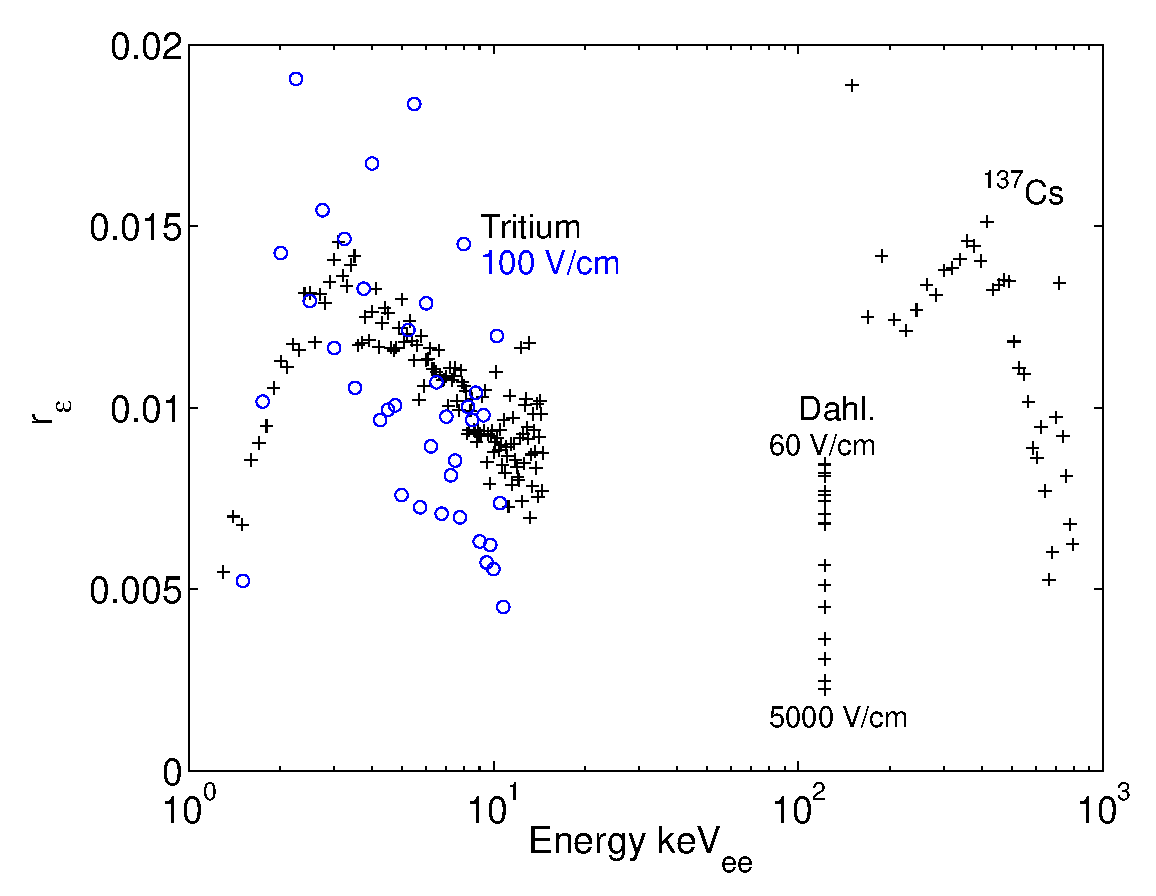
\includegraphics[width=120mm]{Chapter_Flucs/Figures/Recomb_Flucs/Simple/E_re.eps}}

\bigskip

\subcaptionbox{\label{fig:1b}}{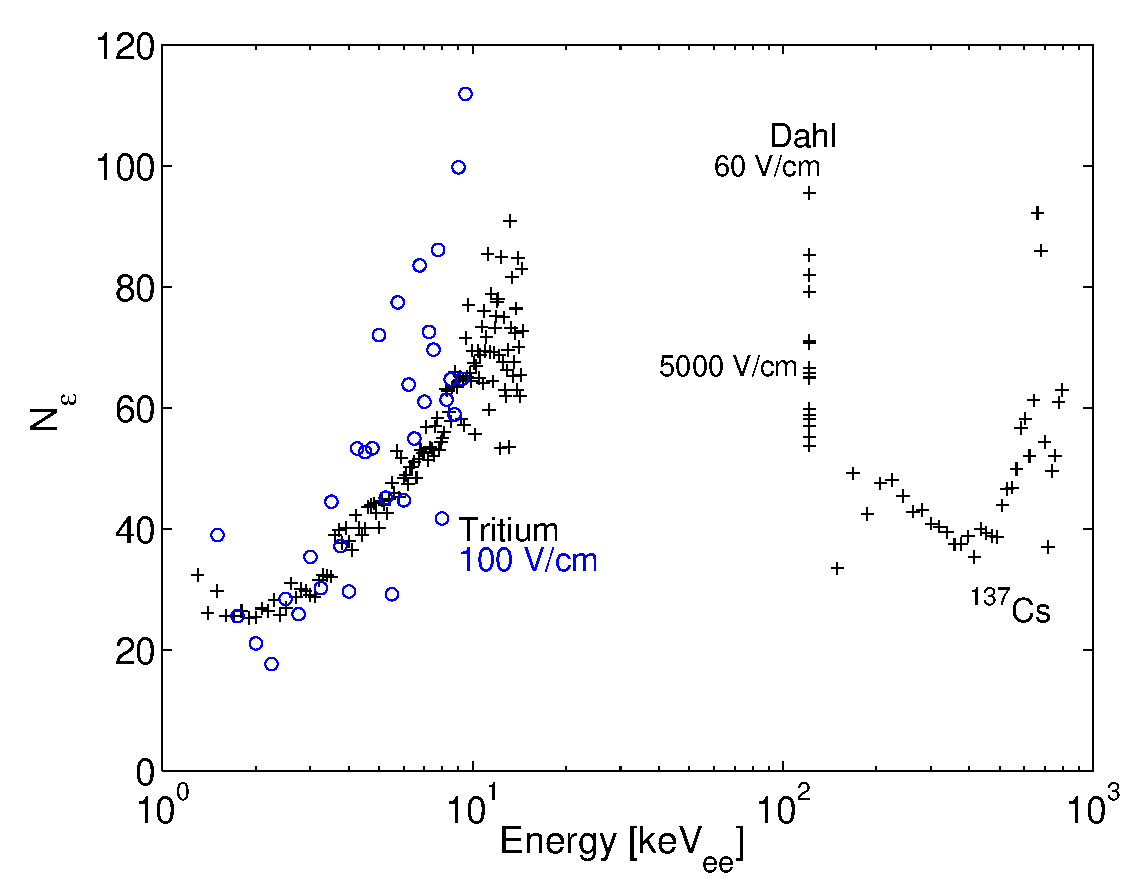
\includegraphics[width=70mm]{Chapter_Flucs/Figures/Recomb_Flucs/Simple/E_Ne.eps}}
\hfill
\subcaptionbox{\label{fig:1b}}{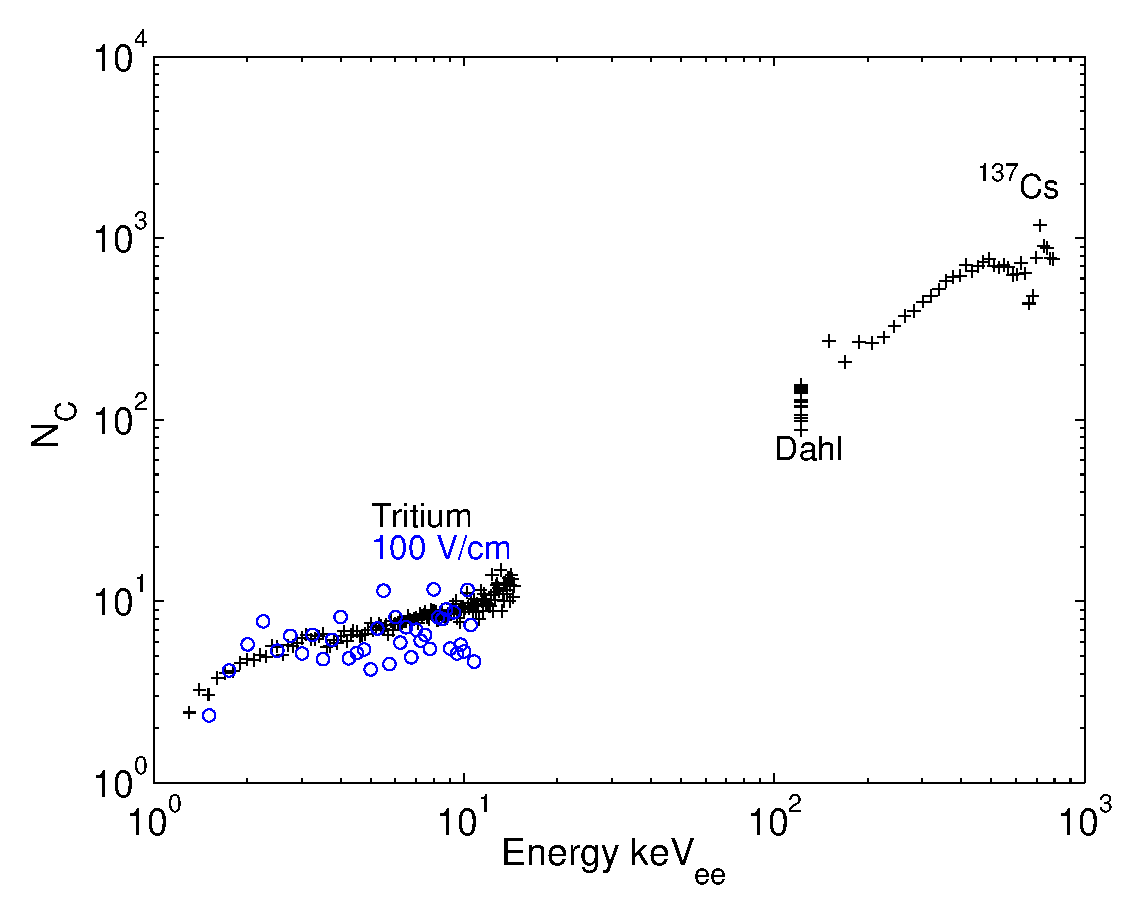
\includegraphics[width=70mm]{Chapter_Flucs/Figures/Recomb_Flucs/Simple/E_clusters.eps}}
\caption{The data shown are labeled on the plot and include calibration data of tritium data at 170 V/cm, tritium at 100 V/cm (blue), $\rm ^{137}Cs$ at 170 V/cm, and data over a rang of fields using $\rm ^{57}Co$ from Dahl. \cite{Dahl_Thesis}. a) The encounter recombination probability $\rm r_\epsilon$ plotted vs. energy. b) The number of encounters per cluster $\rm N_\epsilon$ vs. energy. c) The number of clusters $\rm N_C$ vs. energy.}
\label{fig:Simple_re}
\end{figure}
\renewcommand{\baselinestretch}{2}
\small\normalsize

The average value of $\rm r_\epsilon$ over a wide range of energies is found to be 0.01, shown in figure \ref{fig:Simple_re}. The value of  $\rm r_\epsilon$ determined by using the cluster-encounter model is consistent with that noted by Mozumder in 1995 to explain ion fluctuations in liquid xenon \cite{Mozumder}. The value of  $\rm r_\epsilon=0.01$ corresponds to an average value of encounters $\rm N_\epsilon = 50$, which can be thought of as the cluster size. Figure \ref{fig:Simple_re} (c) also shows the number of clusters vs. energy, which grows linearly with $\rm N_i$.  Note, the number of clusters is the factor by which the binomial fluctuations of the initial self-recombination model are amplified at at given energy.


The number of interaction per cluster $\rm N_\epsilon$, or cluster size, sets the encounter probability $\rm r_\epsilon$ in this model. The value of $\rm N_\epsilon$ appears to level off around 25 as energy tends to zero and varies between 25 to 100 over a wide range of energies and electric fields. Both $\rm r_\epsilon$ and $\rm N_\epsilon$ appear to have dependencies on electric field and energy . Which is not surprising as both the track geometry and interaction probability depend on electric field and energy. The data from Dahl over the range of 60 to 5000 V/cm especially illuminates the dependancies vs. field. We proceed with a simplified model and take the value of  $\rm N_\epsilon$ as a constant. The average value of $\rm N_\epsilon =50$ is used to calculate the expected variance at each energy using equation \ref{eq:Simp_Amp}, the result is shown in figure \ref{fig:Flucs_Simple}.

\newpage 

\renewcommand{\baselinestretch}{1}
\small\normalsize
\begin{figure}[h!]\centering
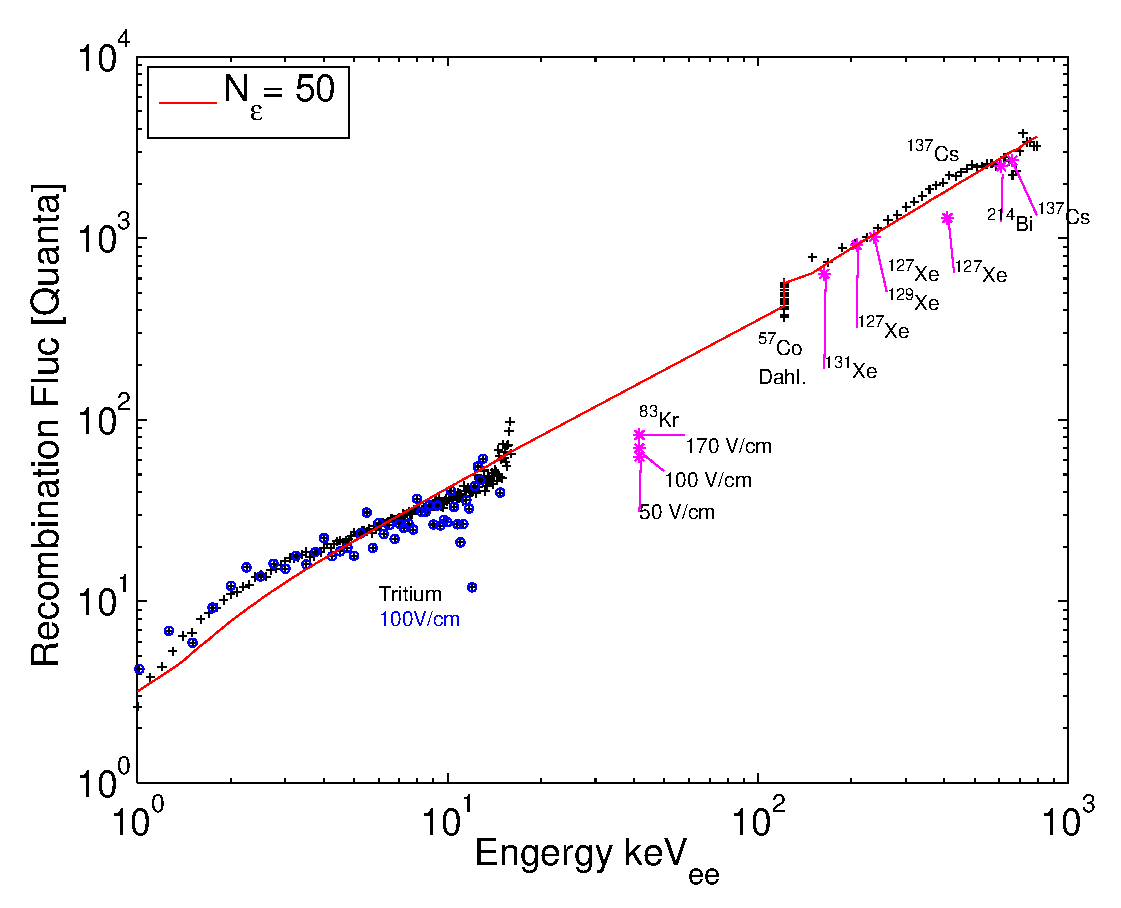
\includegraphics[width=150mm]{Chapter_Flucs/Figures/Recomb_Flucs/Simple/R_v_E_model_stupid_simple_iter1.eps}
\caption{ The measured recombination fluctuations from calibration data vs. energy. The red line indicates the expected recombination fluctuation of the clustering model given in equation \ref{eq:SimpVar_C_2}, assuming a cluster size of $\rm N_\epsilon = 50$. $\rm N_\epsilon = 50$ corresponds to an average encounter recombination probability of $\rm r_\epsilon = 0.01$. The deviation of the fit from the data is less than 30\%. The \KrCal data point is the result of two decays and is expected to fall below the curve by 40\% considering the sum of the individual variances.}
\label{fig:Flucs_Simple}
\end{figure}
\renewcommand{\baselinestretch}{2}
\small\normalsize

\noindent Figure \ref{fig:Flucs_Simple} shows the measured recombination fluctuations vs. energy along with that expected for the clustering model given in equation \ref{eq:SimpVar_C_2}, for $\rm N_\epsilon =50 $, corresponding to an average encounter recombination probability of $\rm r_\epsilon = 0.01$. The deviation of the fit and the data is less than 30\%, including Dahl's data taken at electric fields ranging from 60 to 5000 V/cm. 

With the clustered encounter model we can now account for the recombination fluctuations and understand why recombination tends to zero as energy tends to zero. Having explained these two PEnomena, the clustered-encounter model is a significant improvement over the initial recombination model. The flaw of the initial recombination model was to assume that the recombination process only consists of ion-electron pair self recombination. This assumption is what lead to the observed variance being off by a factor of $\rm N_i$ and the inability to explain the dependance of recombination fraction as energy tends to zero. The picture of ER band mean and width is now complete, only requiring recombination fraction r as an input. The recombination fraction is dependent on the energy of the interaction and electric field, modeled by Thomas \& Imel \cite{Thomas_Imel} and NEST \cite{NEST}, \cite{NEST_2013}. 

\newpage

\section{Conclusion}

%This should be the conclusion after showing the ER band and alpha...

There have been numerous steps in this section culminating in expanding our knowledge by extracting as much information as possible from the calibration sources. We have measured that the best exciton to ion ratio $\rm \alpha$ measured to be 0.20 in the WIMP search energies, which is consistent with the measurement from \cite{Doke_alpha}. The value of alpha was constrained by extrapolating the recombination fluctuations from the tritium data from 3 to 1.2 keV and requiring that for a single ion-electron pair the fluctuation be purely binomial, shown in figure \ref{fig:Alpha_T}.

The recombination model presented in this section can be used to predict the ER band for any xenon detector, as shown in figure \ref{fig:ER_Band_Calc}. The most critical results are those specific to our WIMP search, 10-100 GeV WIMPs, which are focused in the range of 1 to 5 $\rm keV_{ee}$ and well covered by the tritium calibration data. Having extracted the values of r and $\rm \sigma_r$ for ER events the generic mean and band widths can be determined. Thus, the ER band shape can be determined for any xenon detector with the application of the additional variance from the specific detector resolution. The knowledge of this band shape can be used to make predictions about the background rejection power of a given experiment. 

It is surprising to find that changing the drift filed from 100 V/cm to 170 V/cm had only an epsilon impact on the mean of ER band below 4 $\rm keV_{ee}$, figure \ref{fig:ER_Band_Calc}. Further, there was no impact on the energy threshold since the light and charge yields merge at the threshold of 1 keV. A more dramatic field dependance was expected from \cite{Dahl_Thesis} and \cite{NEST_2013}. However, the low energy region never been probed to such high precision as with the tritium calibration using the LUX detector. To expand upon the modeling at low energies it will be useful for the next science run using the LUX detector to take tritium calibration data at a verity of fields. This will allow us to predict exactly how much additional NR and ER discrimination can be achieved by increasing the field. %We also want to explore if the recombination fluctuation can truly be thought of an an amplification of the variance over that of the underlying binomial process of electron-ion pair recombination.
